\begin{figure*}
  \begin{minipage}{0.5\columnwidth}
    \centering
    Generations Ago (approx.)
  \end{minipage}
  \hfill
  \begin{minipage}{0.5\columnwidth}
    \centering
    Generations Ago (approx.)
  \end{minipage}
  \begin{minipage}{0.5\columnwidth}
    \hspace{0.02\linewidth}
    \rotatebox{30}{\makebox[0.1\linewidth][c]{200,000}}
    \hfill
    \rotatebox{30}{\makebox[0.1\linewidth][c]{150,000}}
    \hfill
    \rotatebox{30}{\makebox[0.1\linewidth][c]{100,000}}
    \hfill
    \rotatebox{30}{\makebox[0.1\linewidth][c]{50,000}}
    \hfill
    \rotatebox{90}{\makebox[0.05\linewidth][c]{0}}
  \end{minipage}
  \hfill
  \begin{minipage}{0.5\columnwidth}
    \hspace{0.02\linewidth}
    \rotatebox{30}{\makebox[0.1\linewidth][c]{200,000}}
    \hfill
    \rotatebox{30}{\makebox[0.1\linewidth][c]{150,000}}
    \hfill
    \rotatebox{30}{\makebox[0.1\linewidth][c]{100,000}}
    \hfill
    \rotatebox{30}{\makebox[0.1\linewidth][c]{50,000}}
    \hfill
    \rotatebox{90}{\makebox[0.05\linewidth][c]{0}}
  \end{minipage}
  \hfill
  \begin{subfigure}[b]{0.5\columnwidth}
    % \begin{noindent}
    % 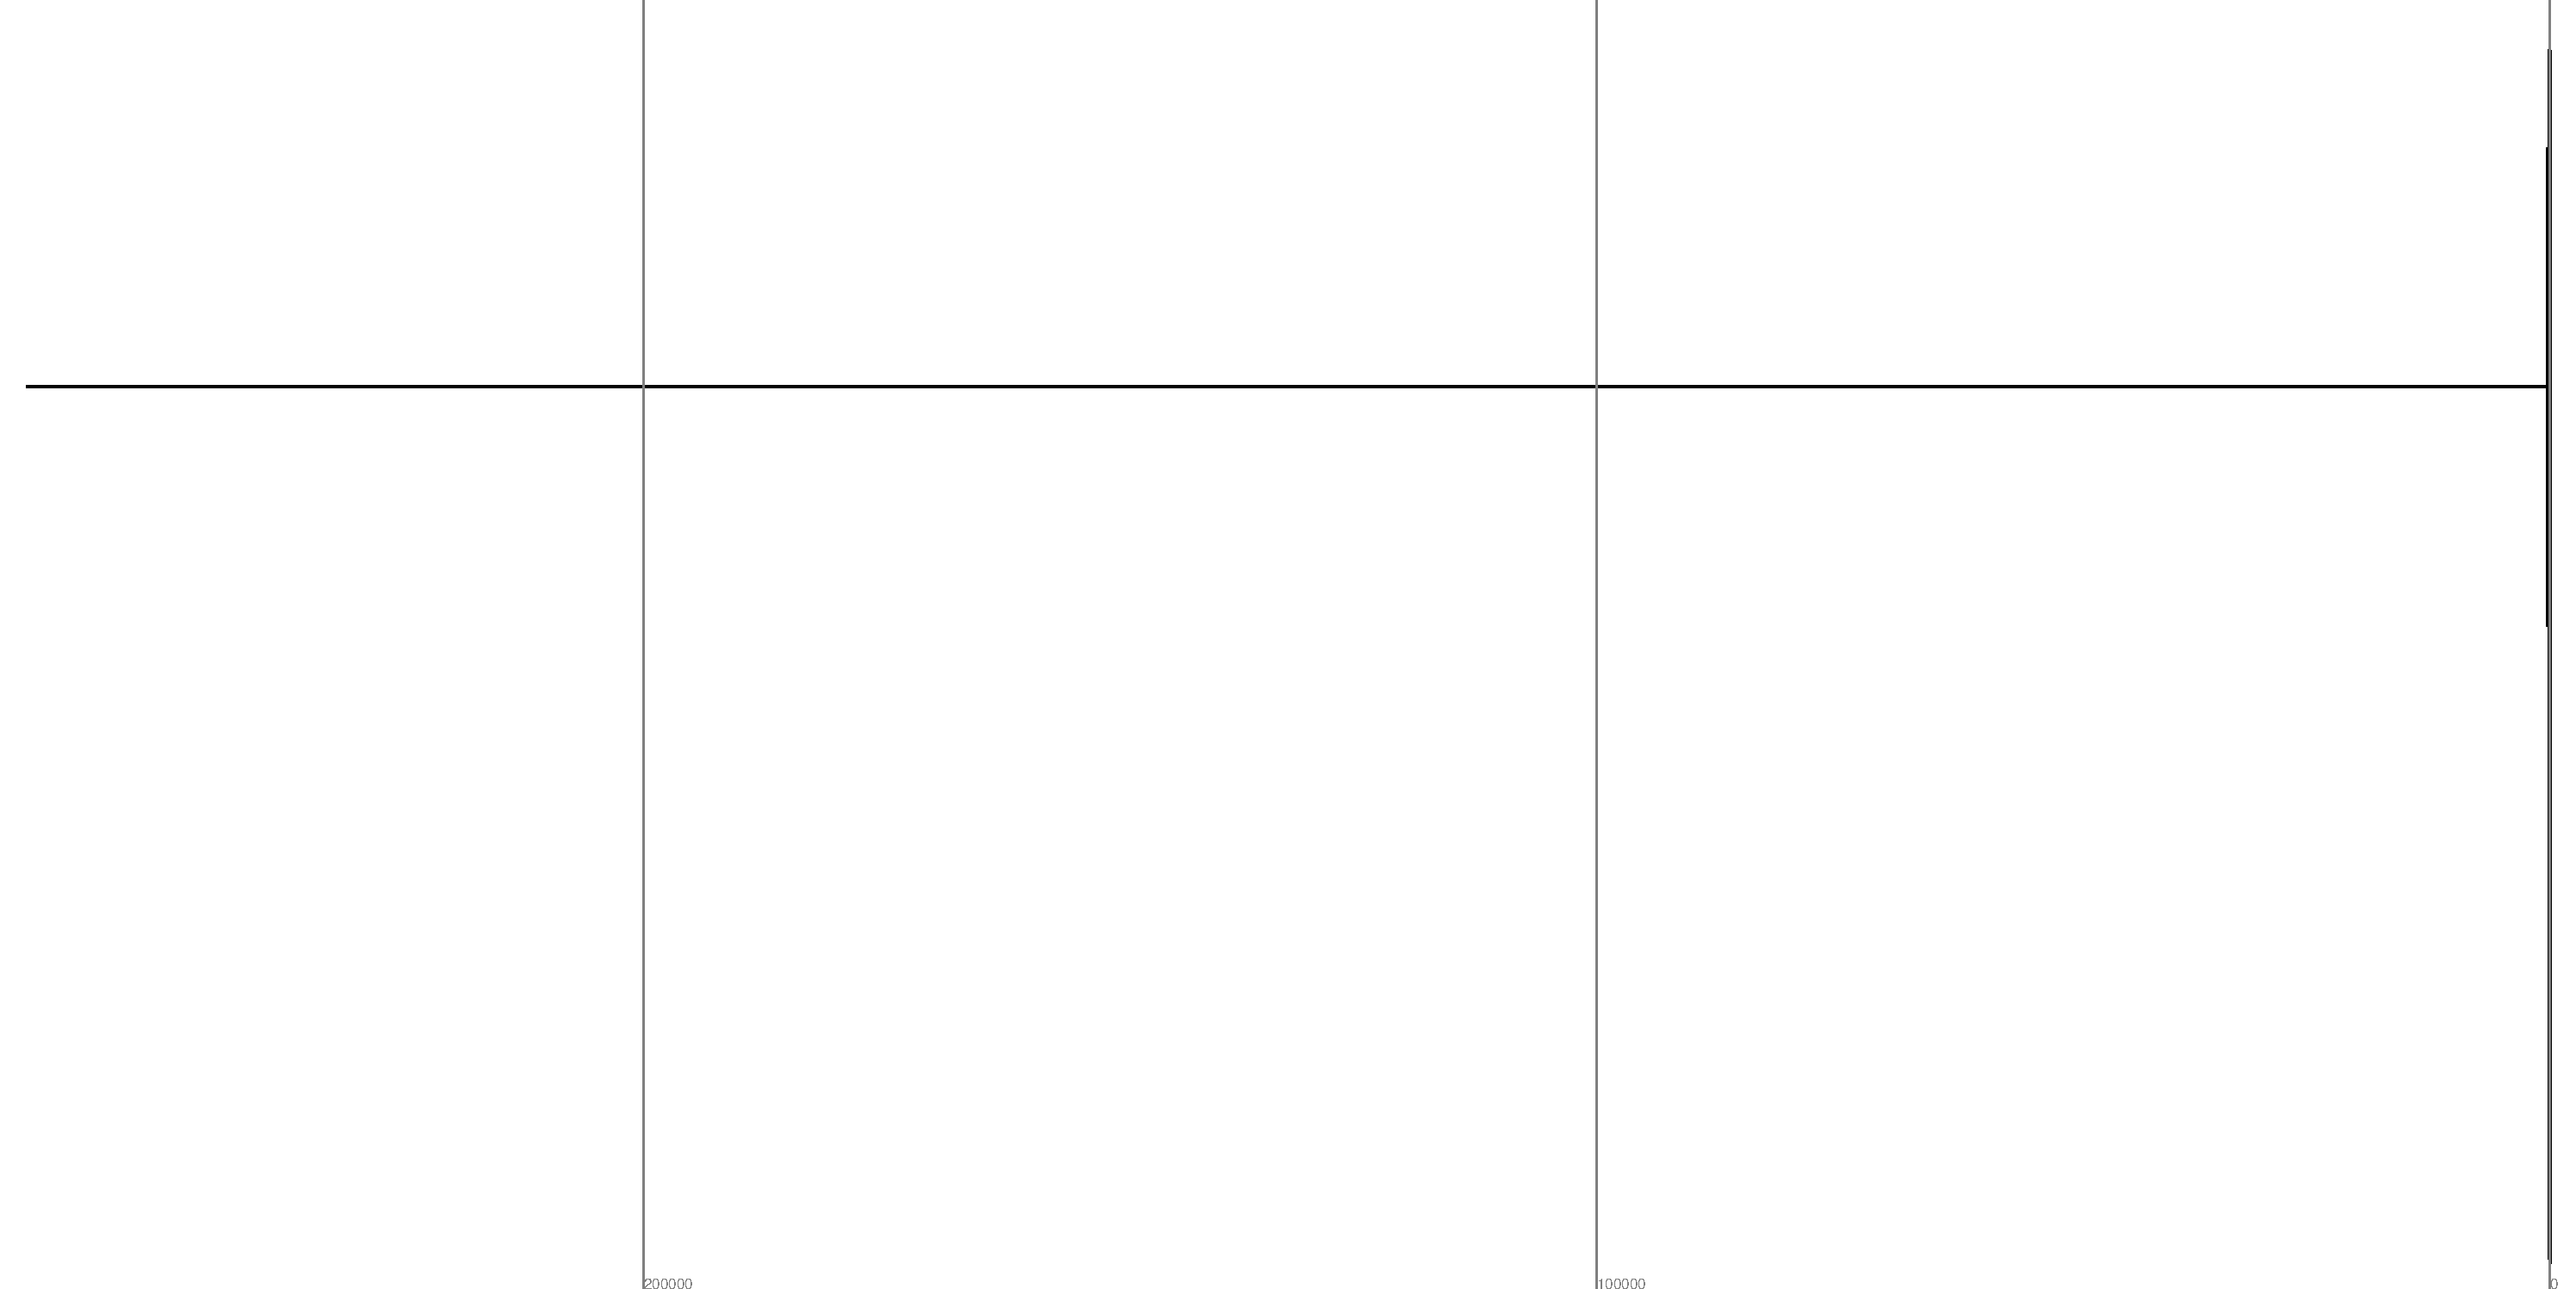
\includegraphics[height=0.12\textheight,width=\textwidth]{img/perfect-tree-phylogenies-log/epoch=7+resolution=3+treatment=2/a=collapsed-phylogeny+epoch=00007+mut_distn=np.random.standard_normal+num_generations=32768+num_islands=1+num_niches=1+p_island_migration=0.01+p_niche_invasion=3.0517578125e-08+population_size=32768+r.../eplicate=0+tournament_size=4+treatment=2+_generation=262144+_index=2+scale=nonlog+ext=.pdf}
    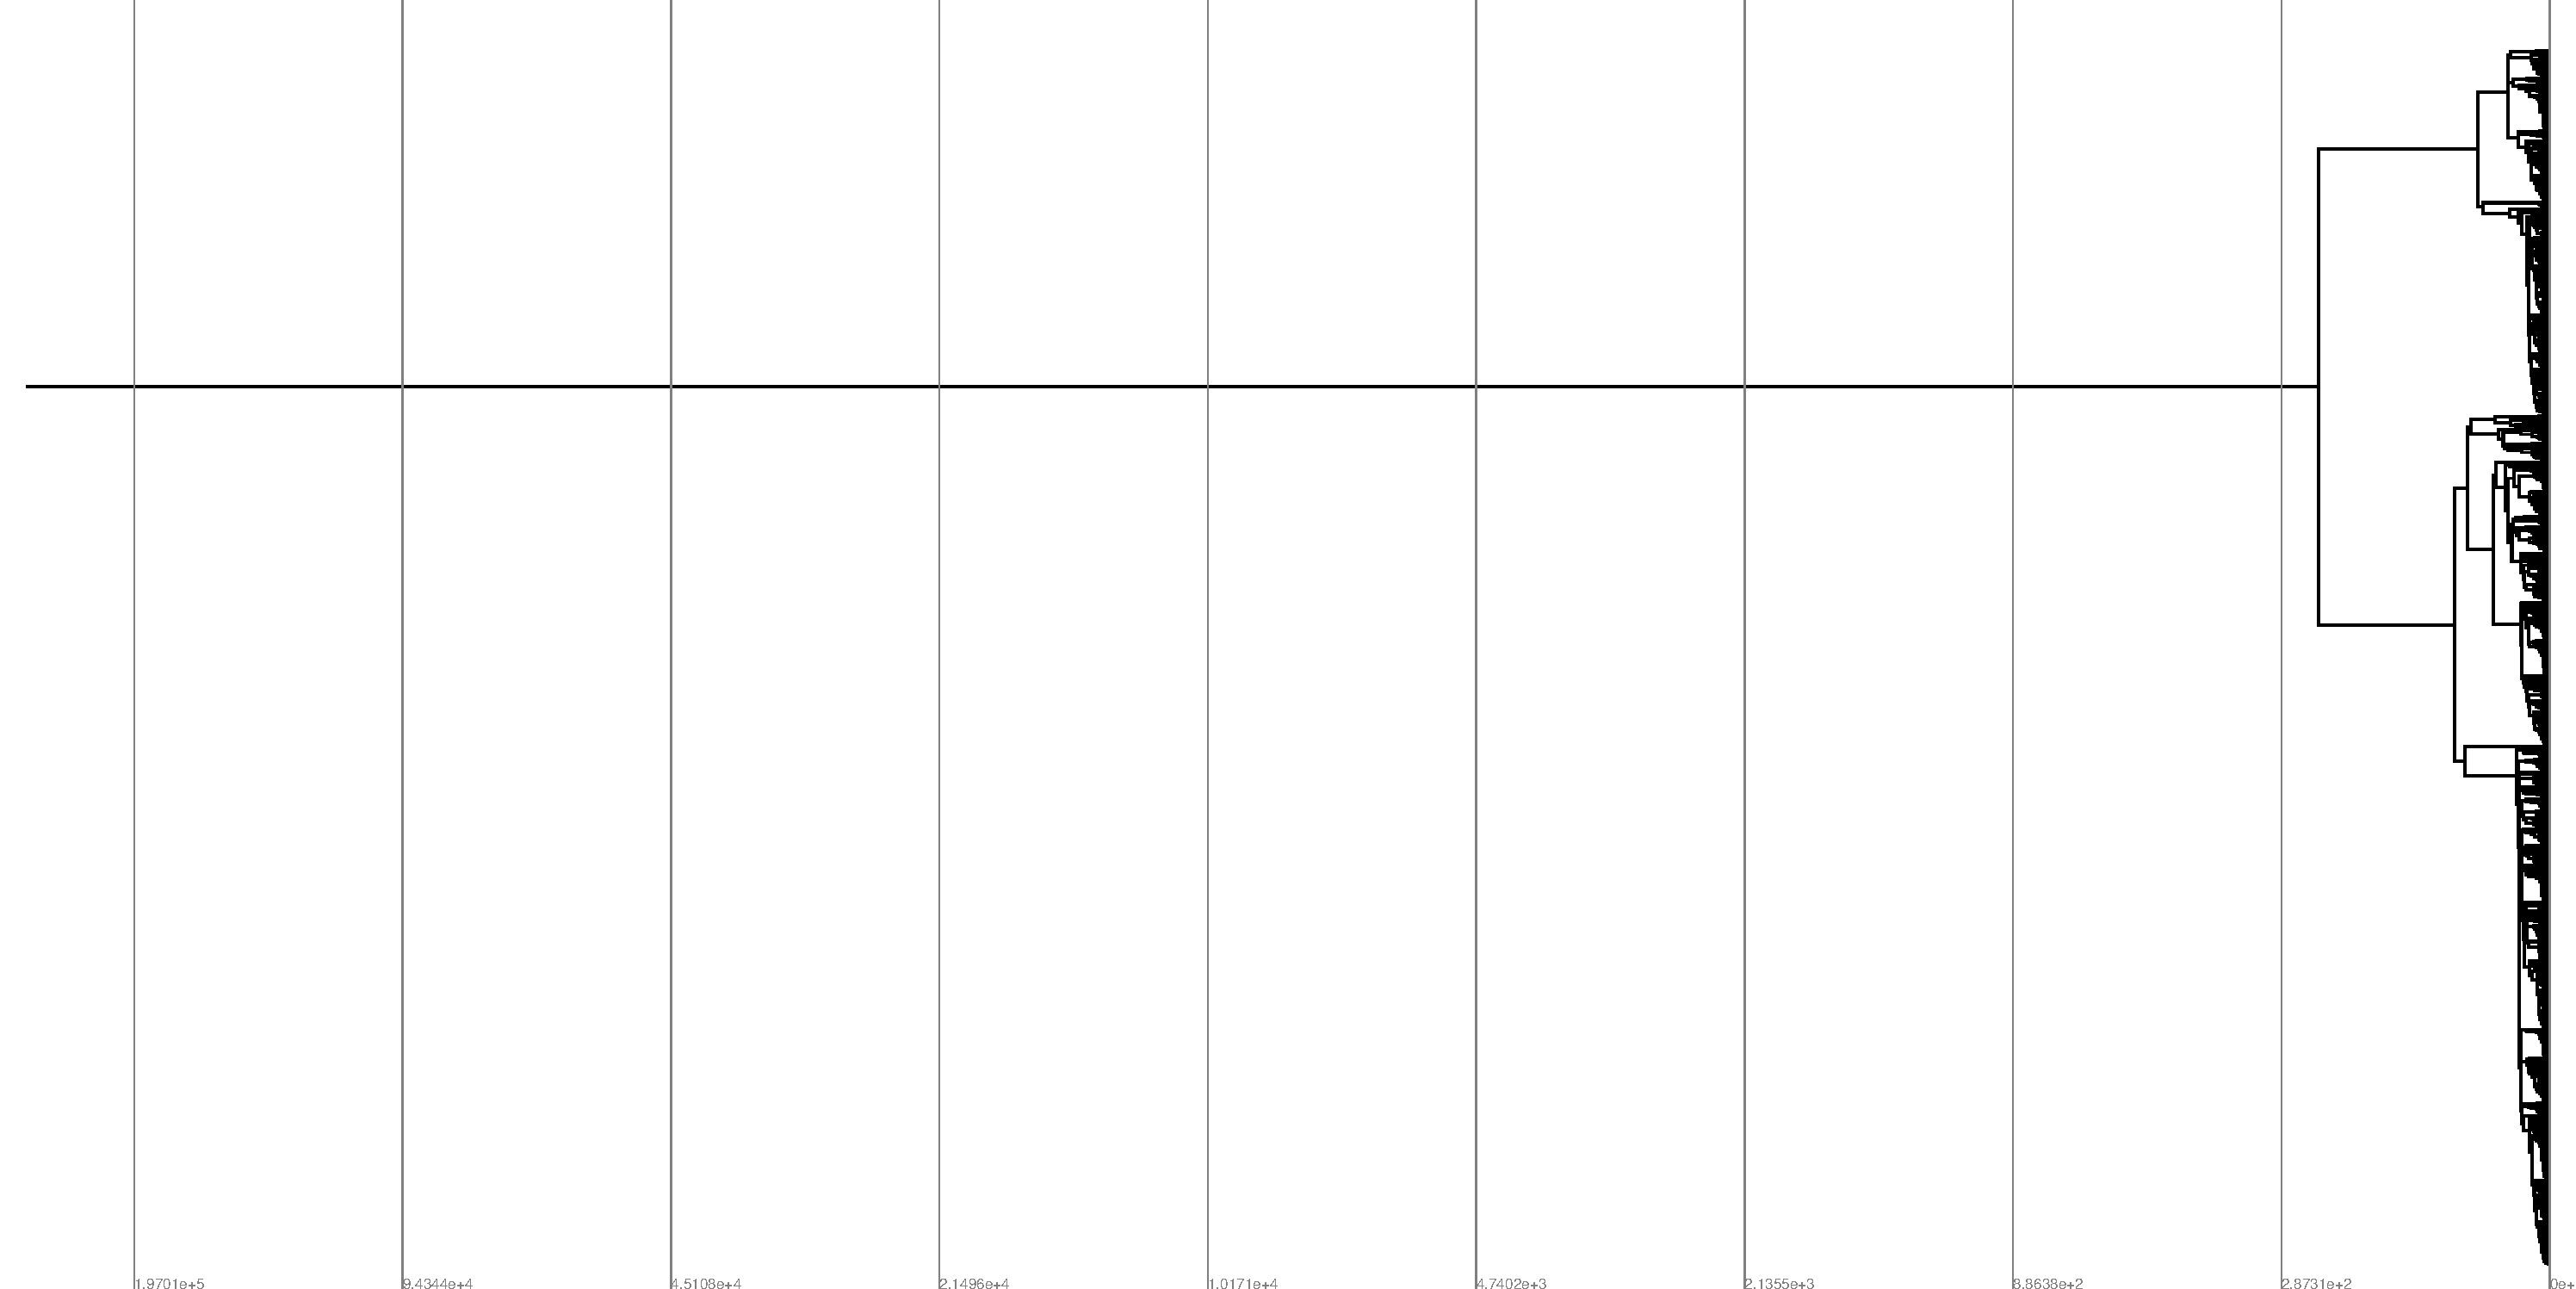
\includegraphics[height=0.12\textheight,width=\textwidth]{img/perfect-tree-phylogenies-log/epoch=7+resolution=3+treatment=2.pdf}
    % \end{noindent}
    \caption{%
      strong selection}
    % \label{fig:perfect-tree-phylogenies-log:TODO}
  \end{subfigure}
  \hfill
  \begin{subfigure}[b]{0.5\columnwidth}
    % \begin{noindent}
    % 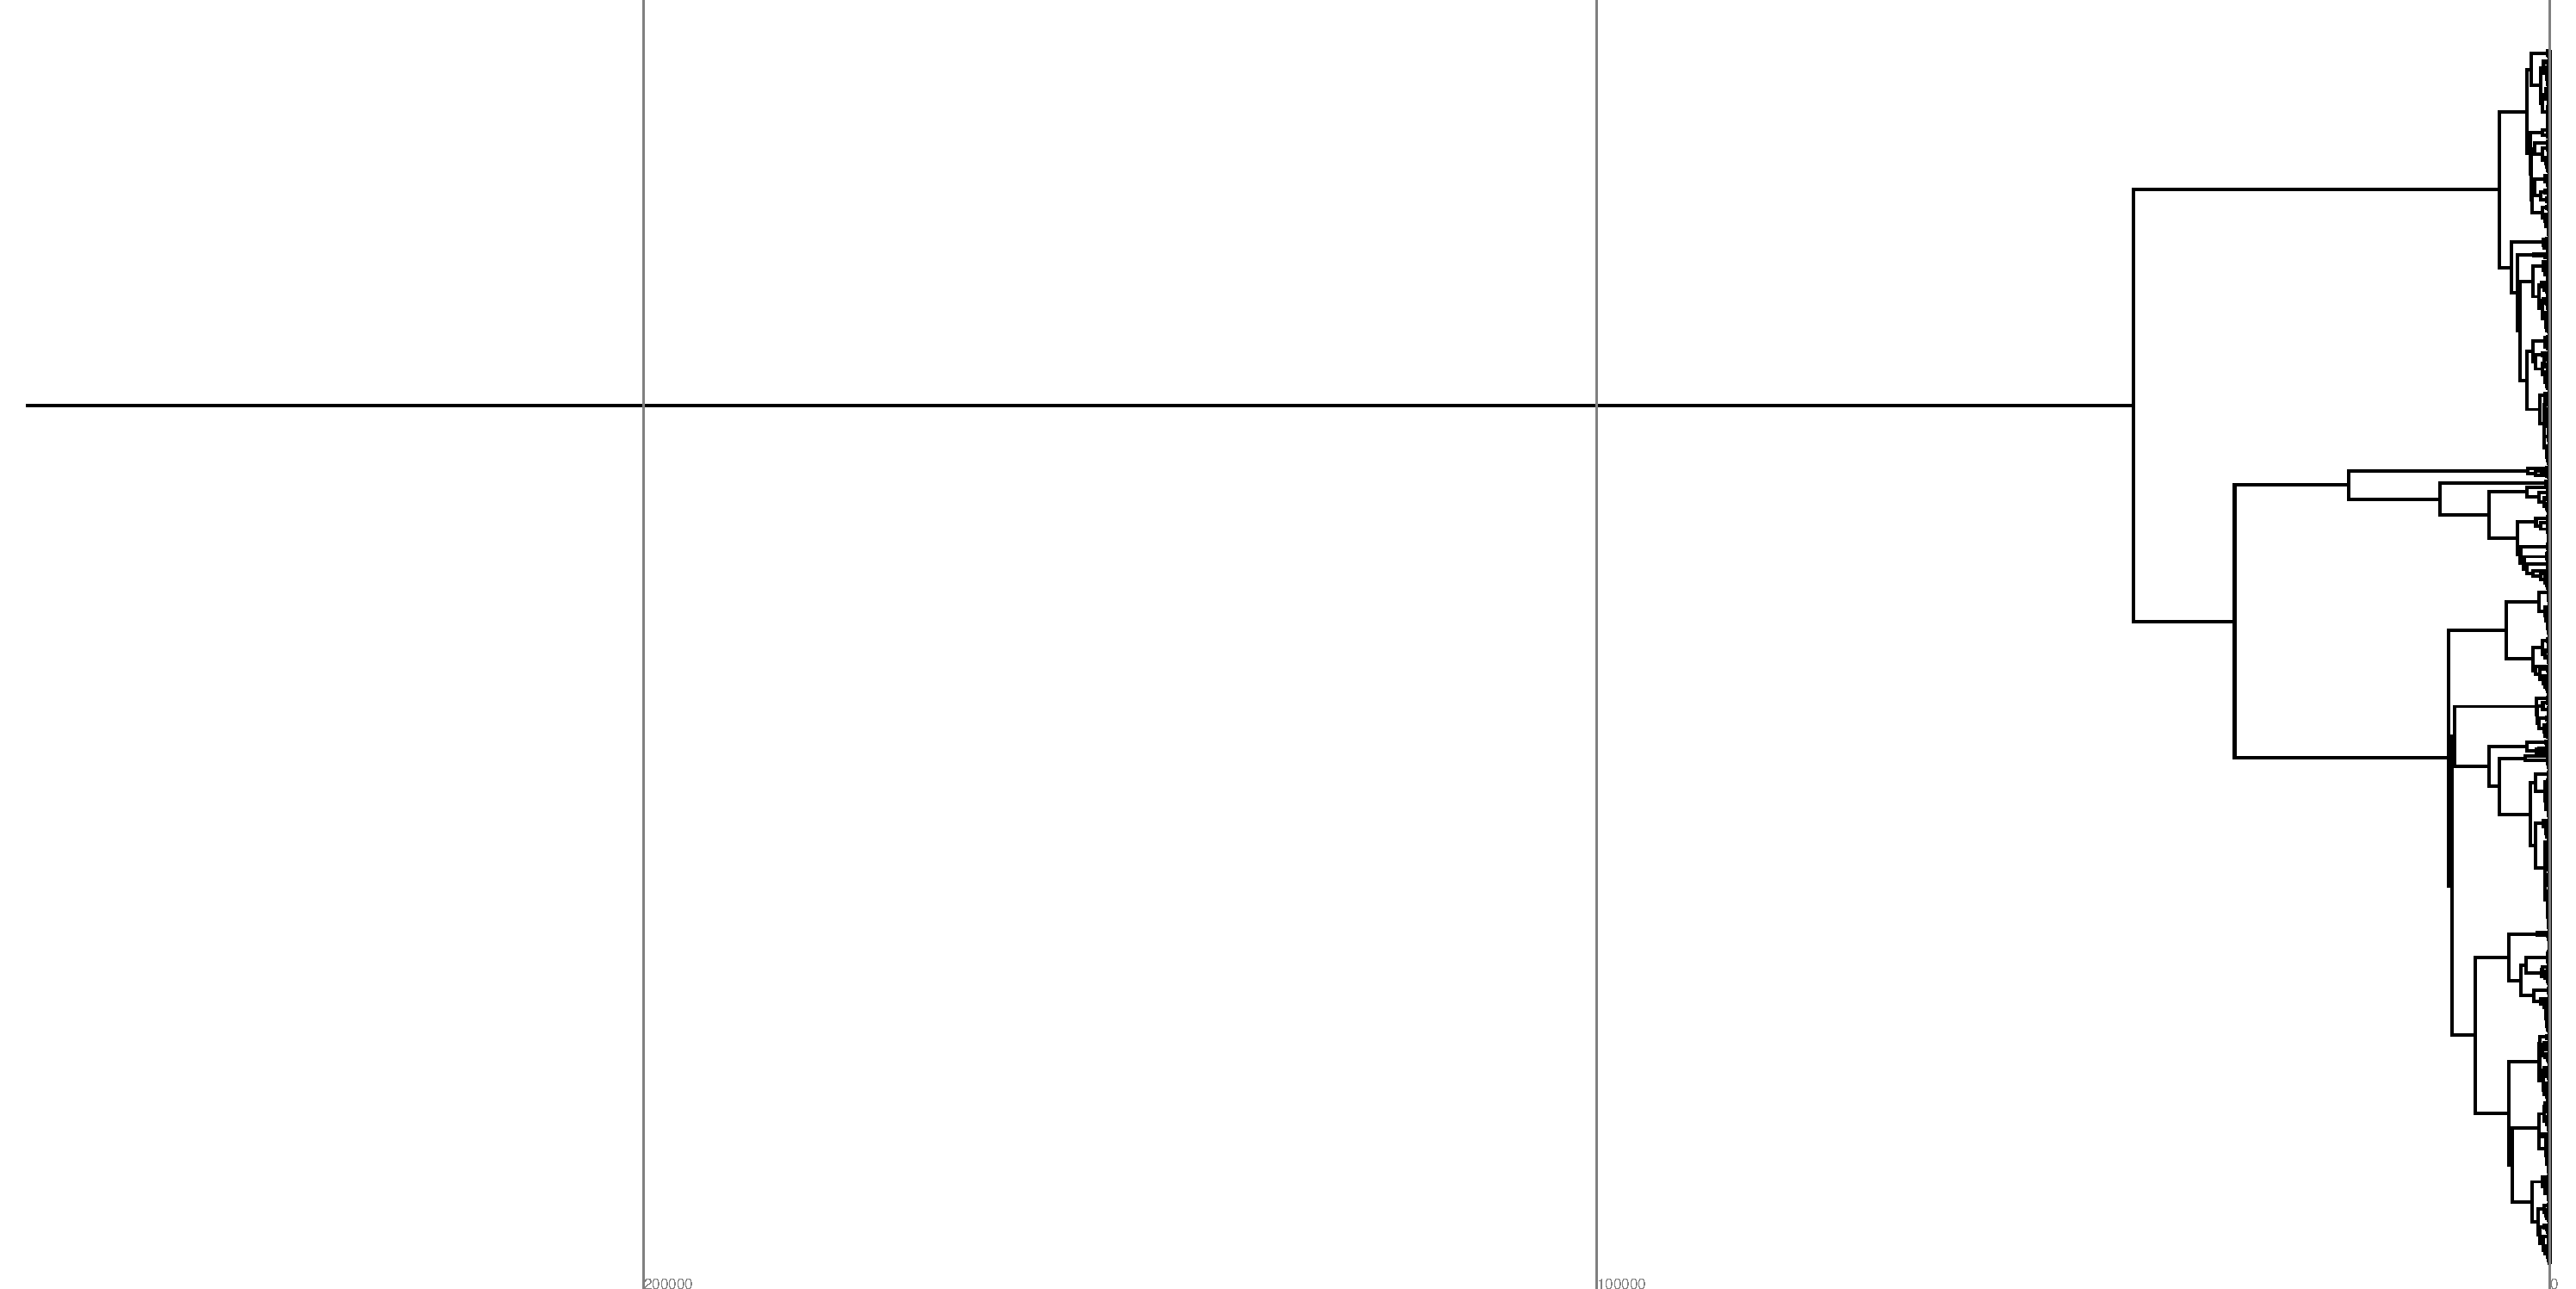
\includegraphics[height=0.12\textheight,width=\textwidth]{img/perfect-tree-phylogenies-log/epoch=7+resolution=3+treatment=14/a=collapsed-phylogeny+epoch=00007+mut_distn=np.random.standard_normal+num_generations=32768+num_islands=1+num_niches=1+p_island_migration=0.01+p_niche_invasion=3.0517578125e-08+population_size=32768+r.../eplicate=0+tournament_size=1+treatment=14+_generation=262144+_index=14+scale=nonlog+ext=.pdf}
    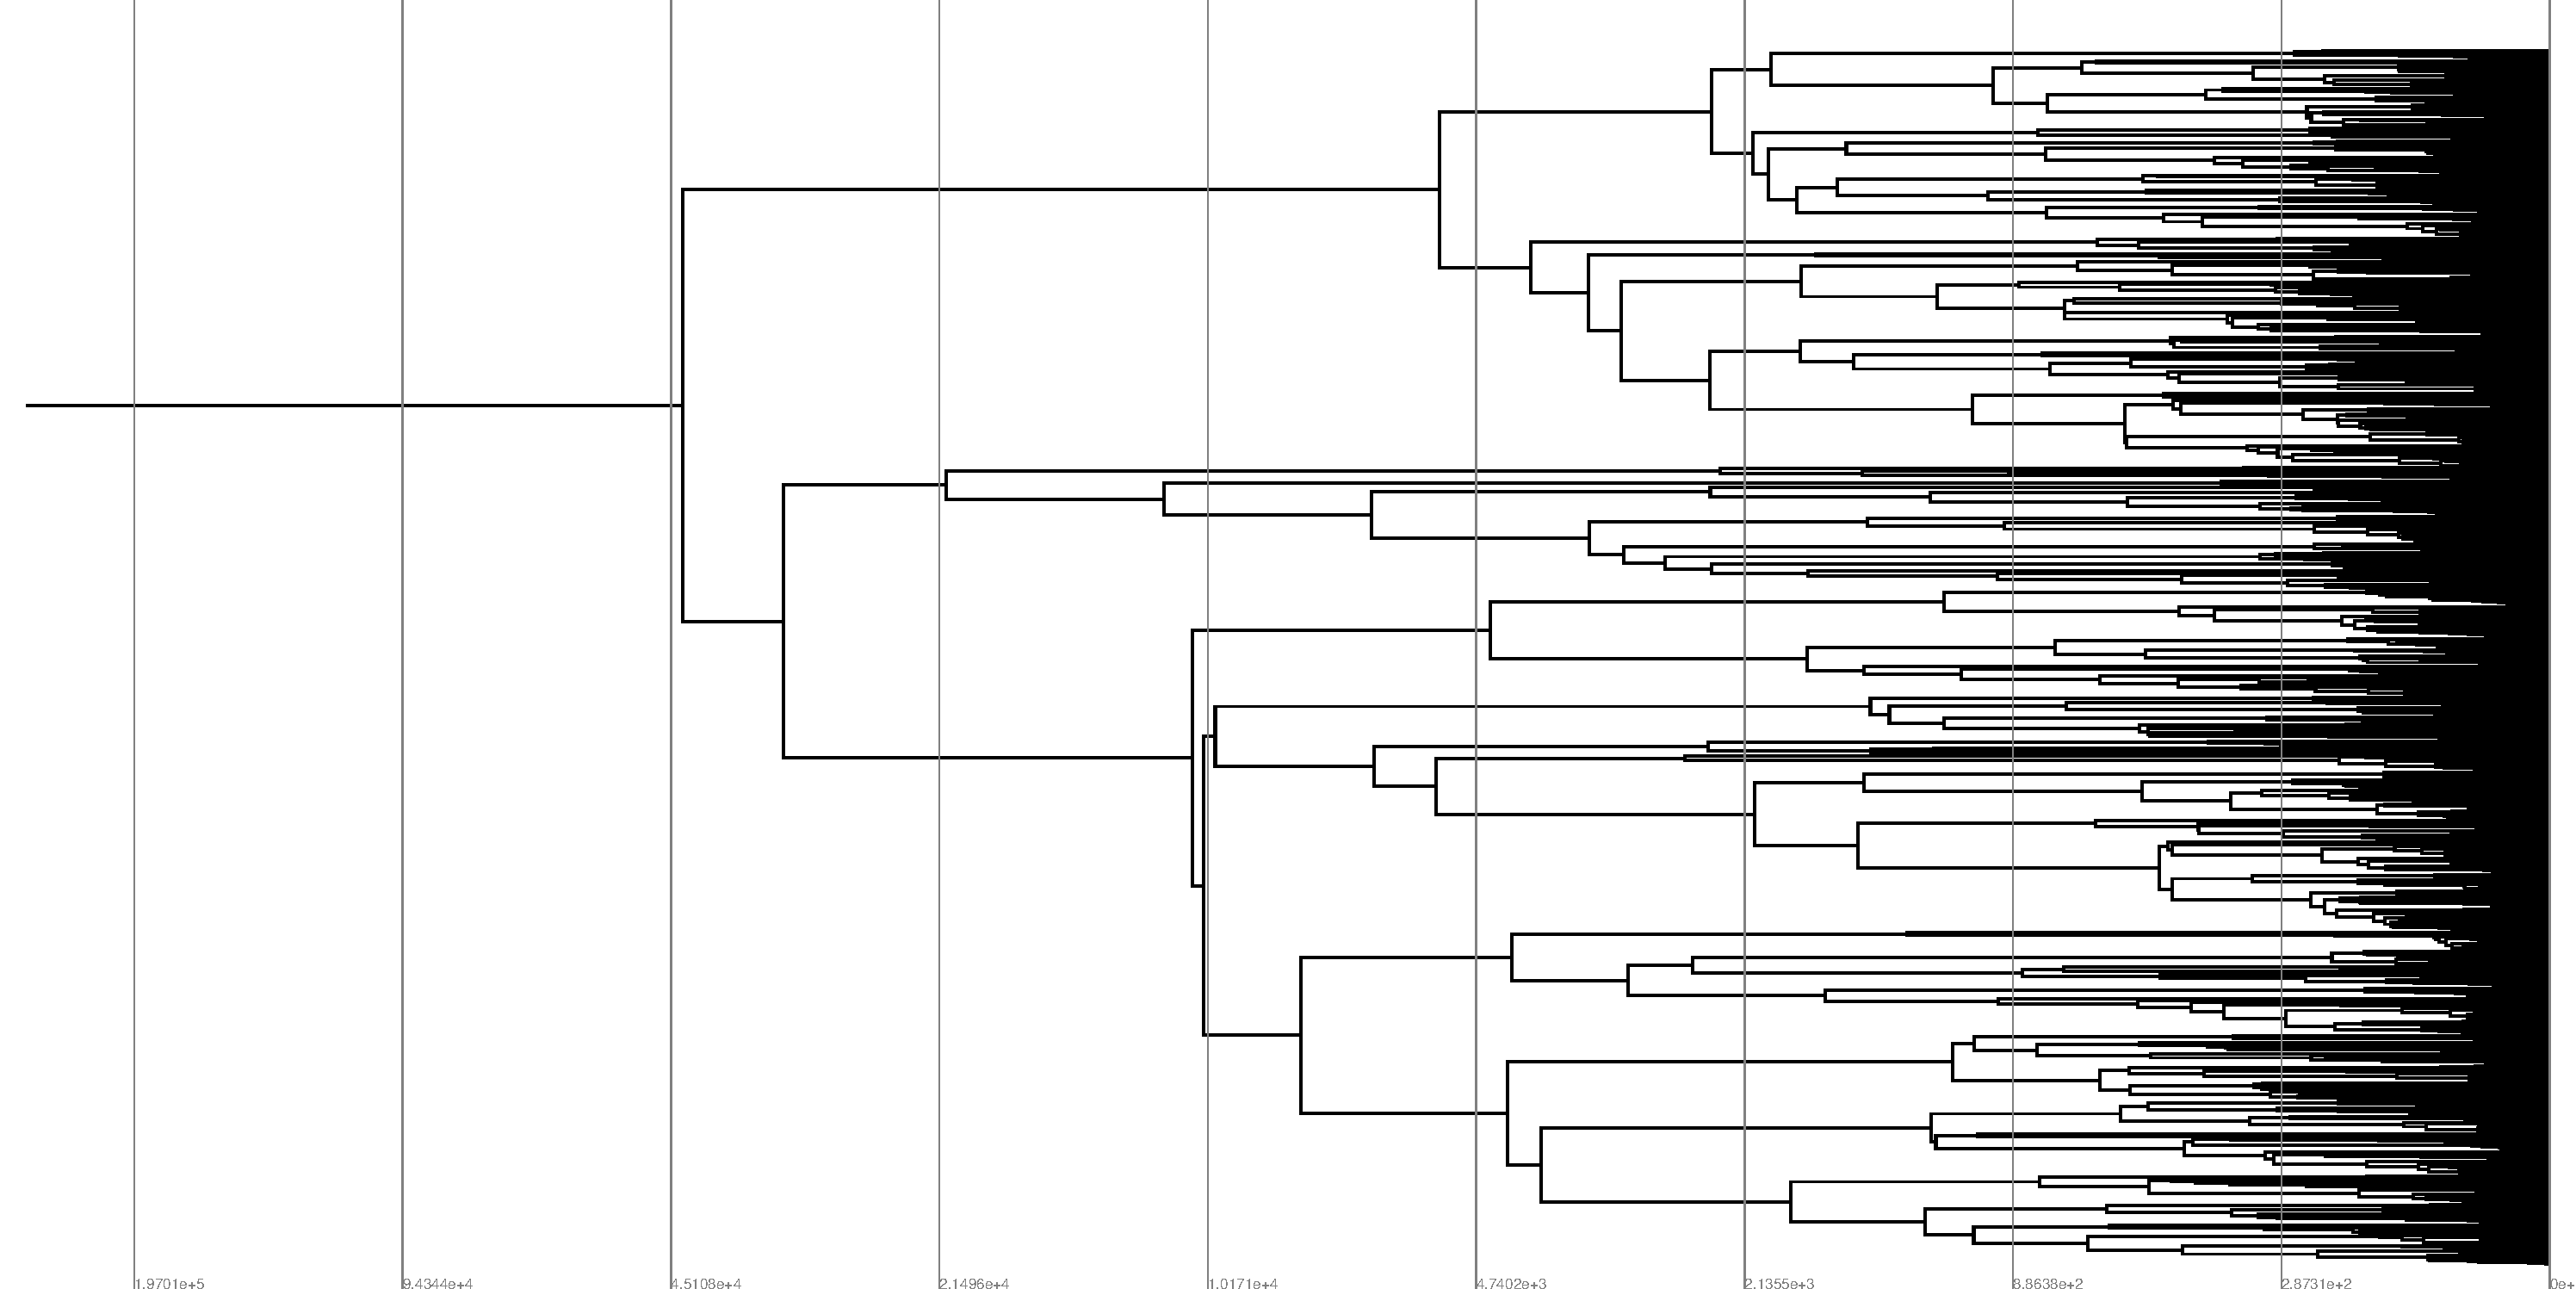
\includegraphics[height=0.12\textheight,width=\textwidth]{img/perfect-tree-phylogenies-log/epoch=7+resolution=3+treatment=14.pdf}
    % \end{noindent}
    \caption{%
      weak selection}
    % \label{fig:perfect-tree-phylogenies-log:TODO}
  \end{subfigure}
  \hfill
  \begin{subfigure}[b]{0.5\columnwidth}
    \centering
    % \begin{noindent}
    % 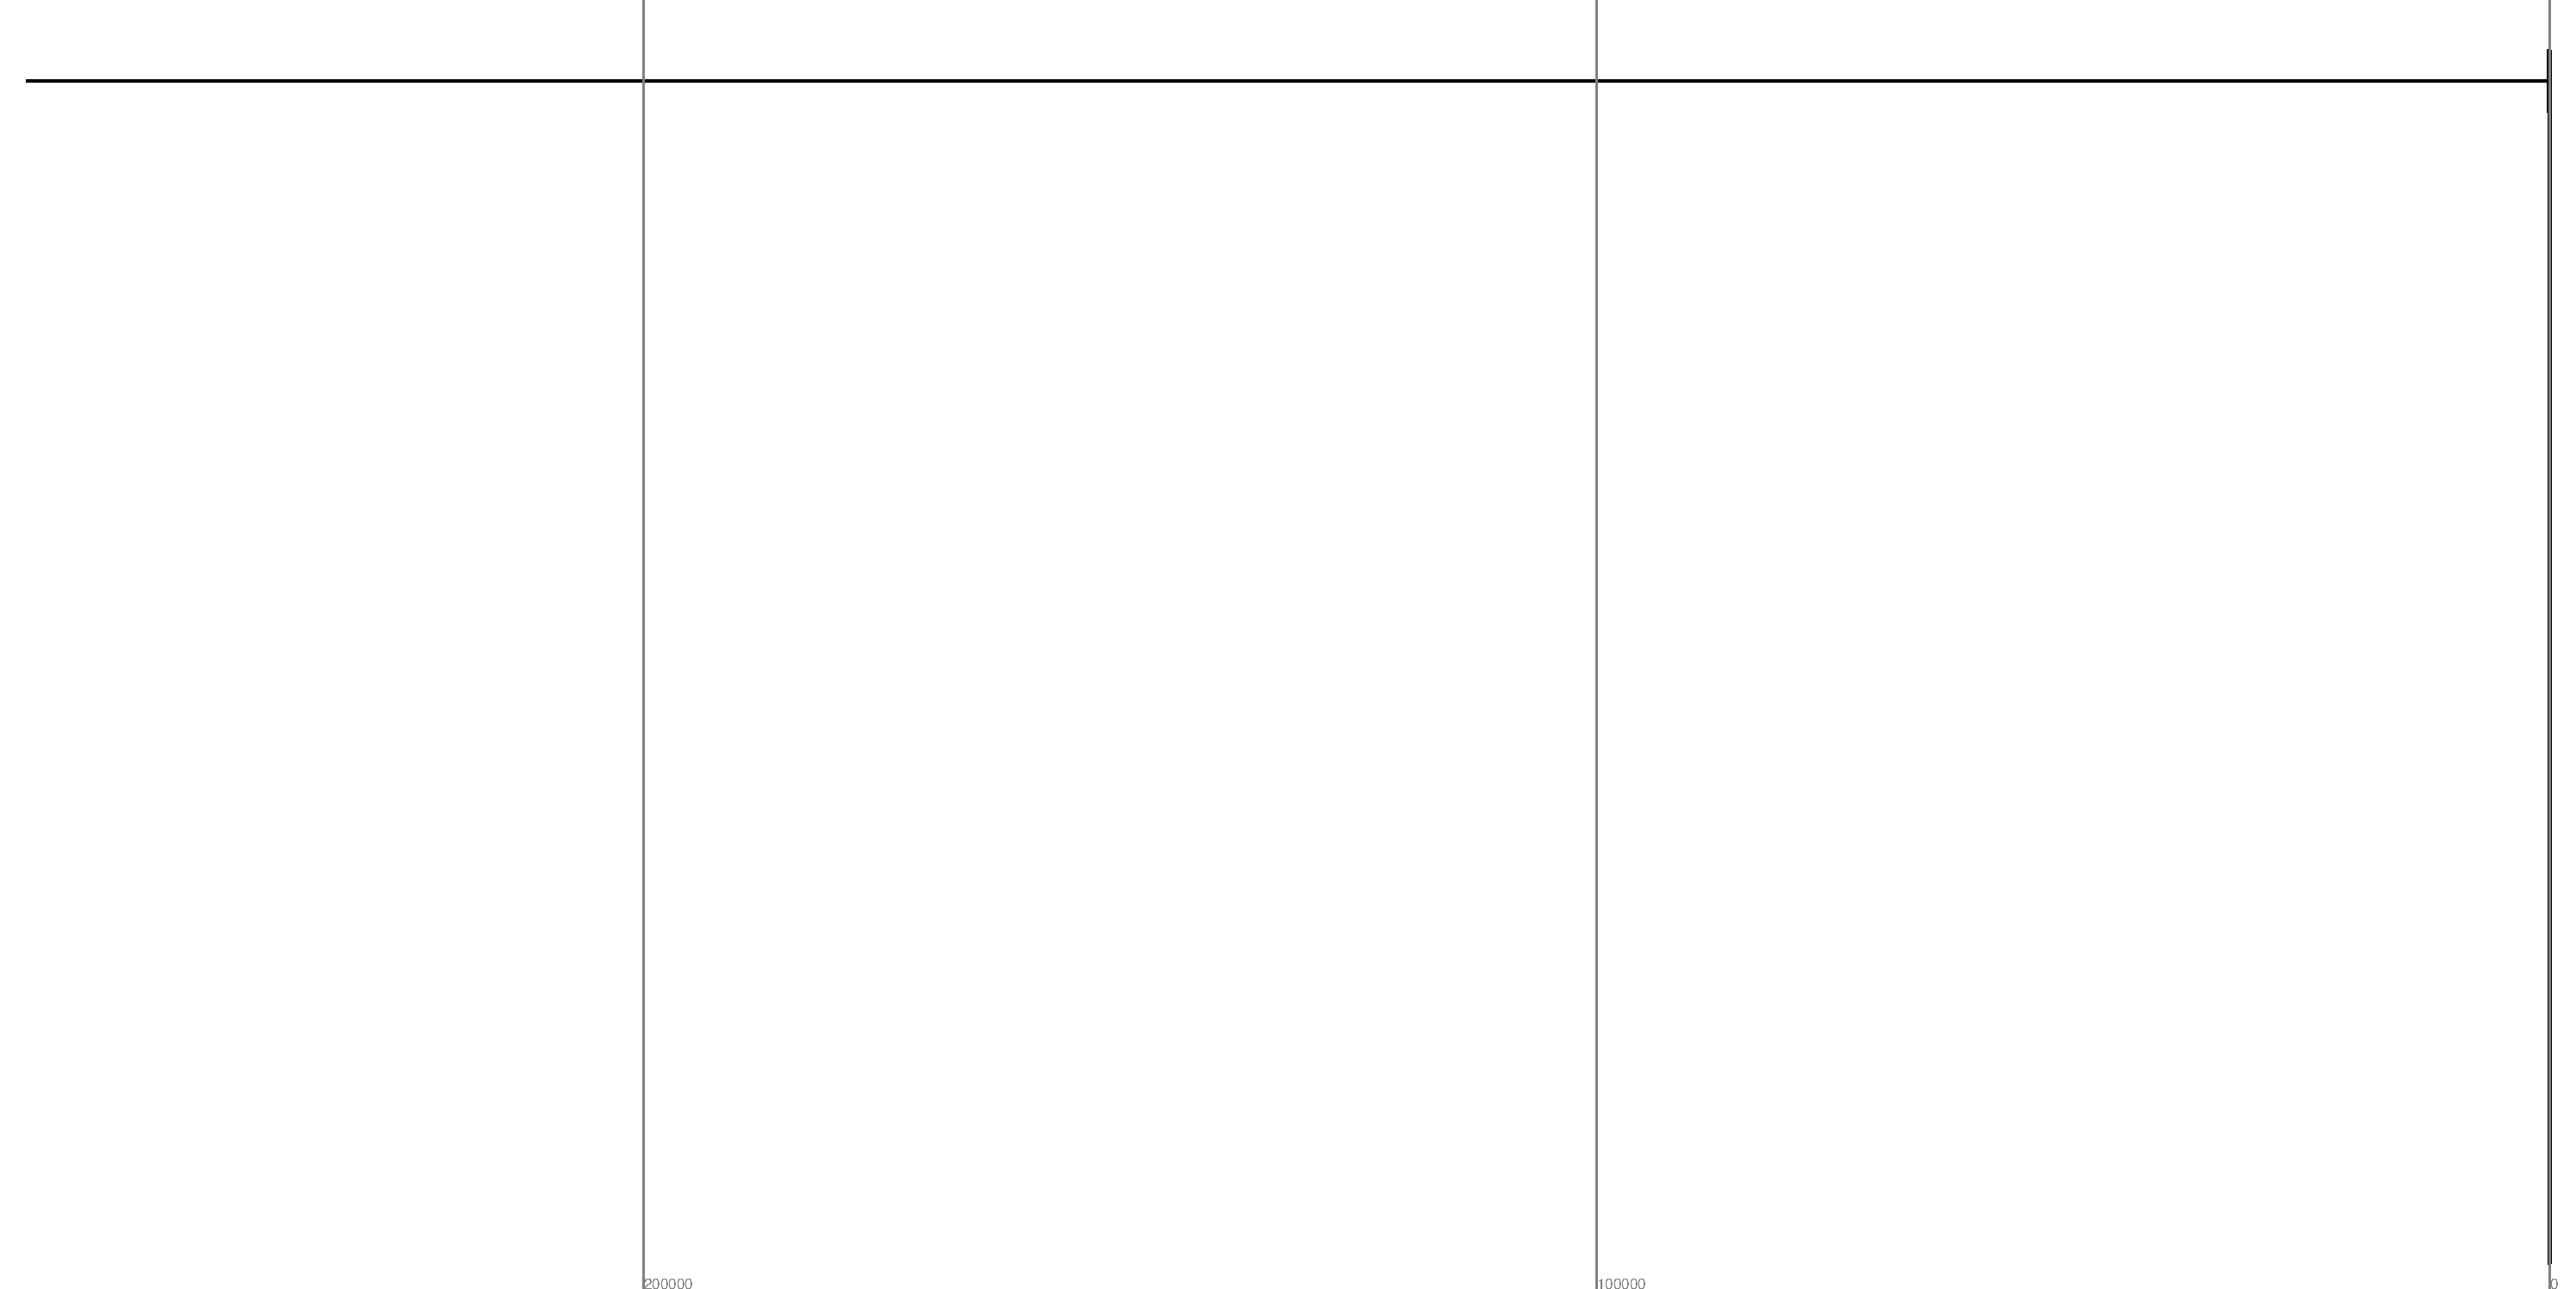
\includegraphics[height=0.12\textheight,width=\textwidth]{img/perfect-tree-phylogenies-log/epoch=7+resolution=3+treatment=8/a=collapsed-phylogeny+epoch=00007+mut_distn=np.random.standard_normal+num_generations=32768+num_islands=1+num_niches=1+p_island_migration=0.01+p_niche_invasion=3.0517578125e-08+population_size=32768+r.../eplicate=0+tournament_size=2+treatment=8+_generation=262144+_index=8+scale=nonlog+ext=.pdf}
    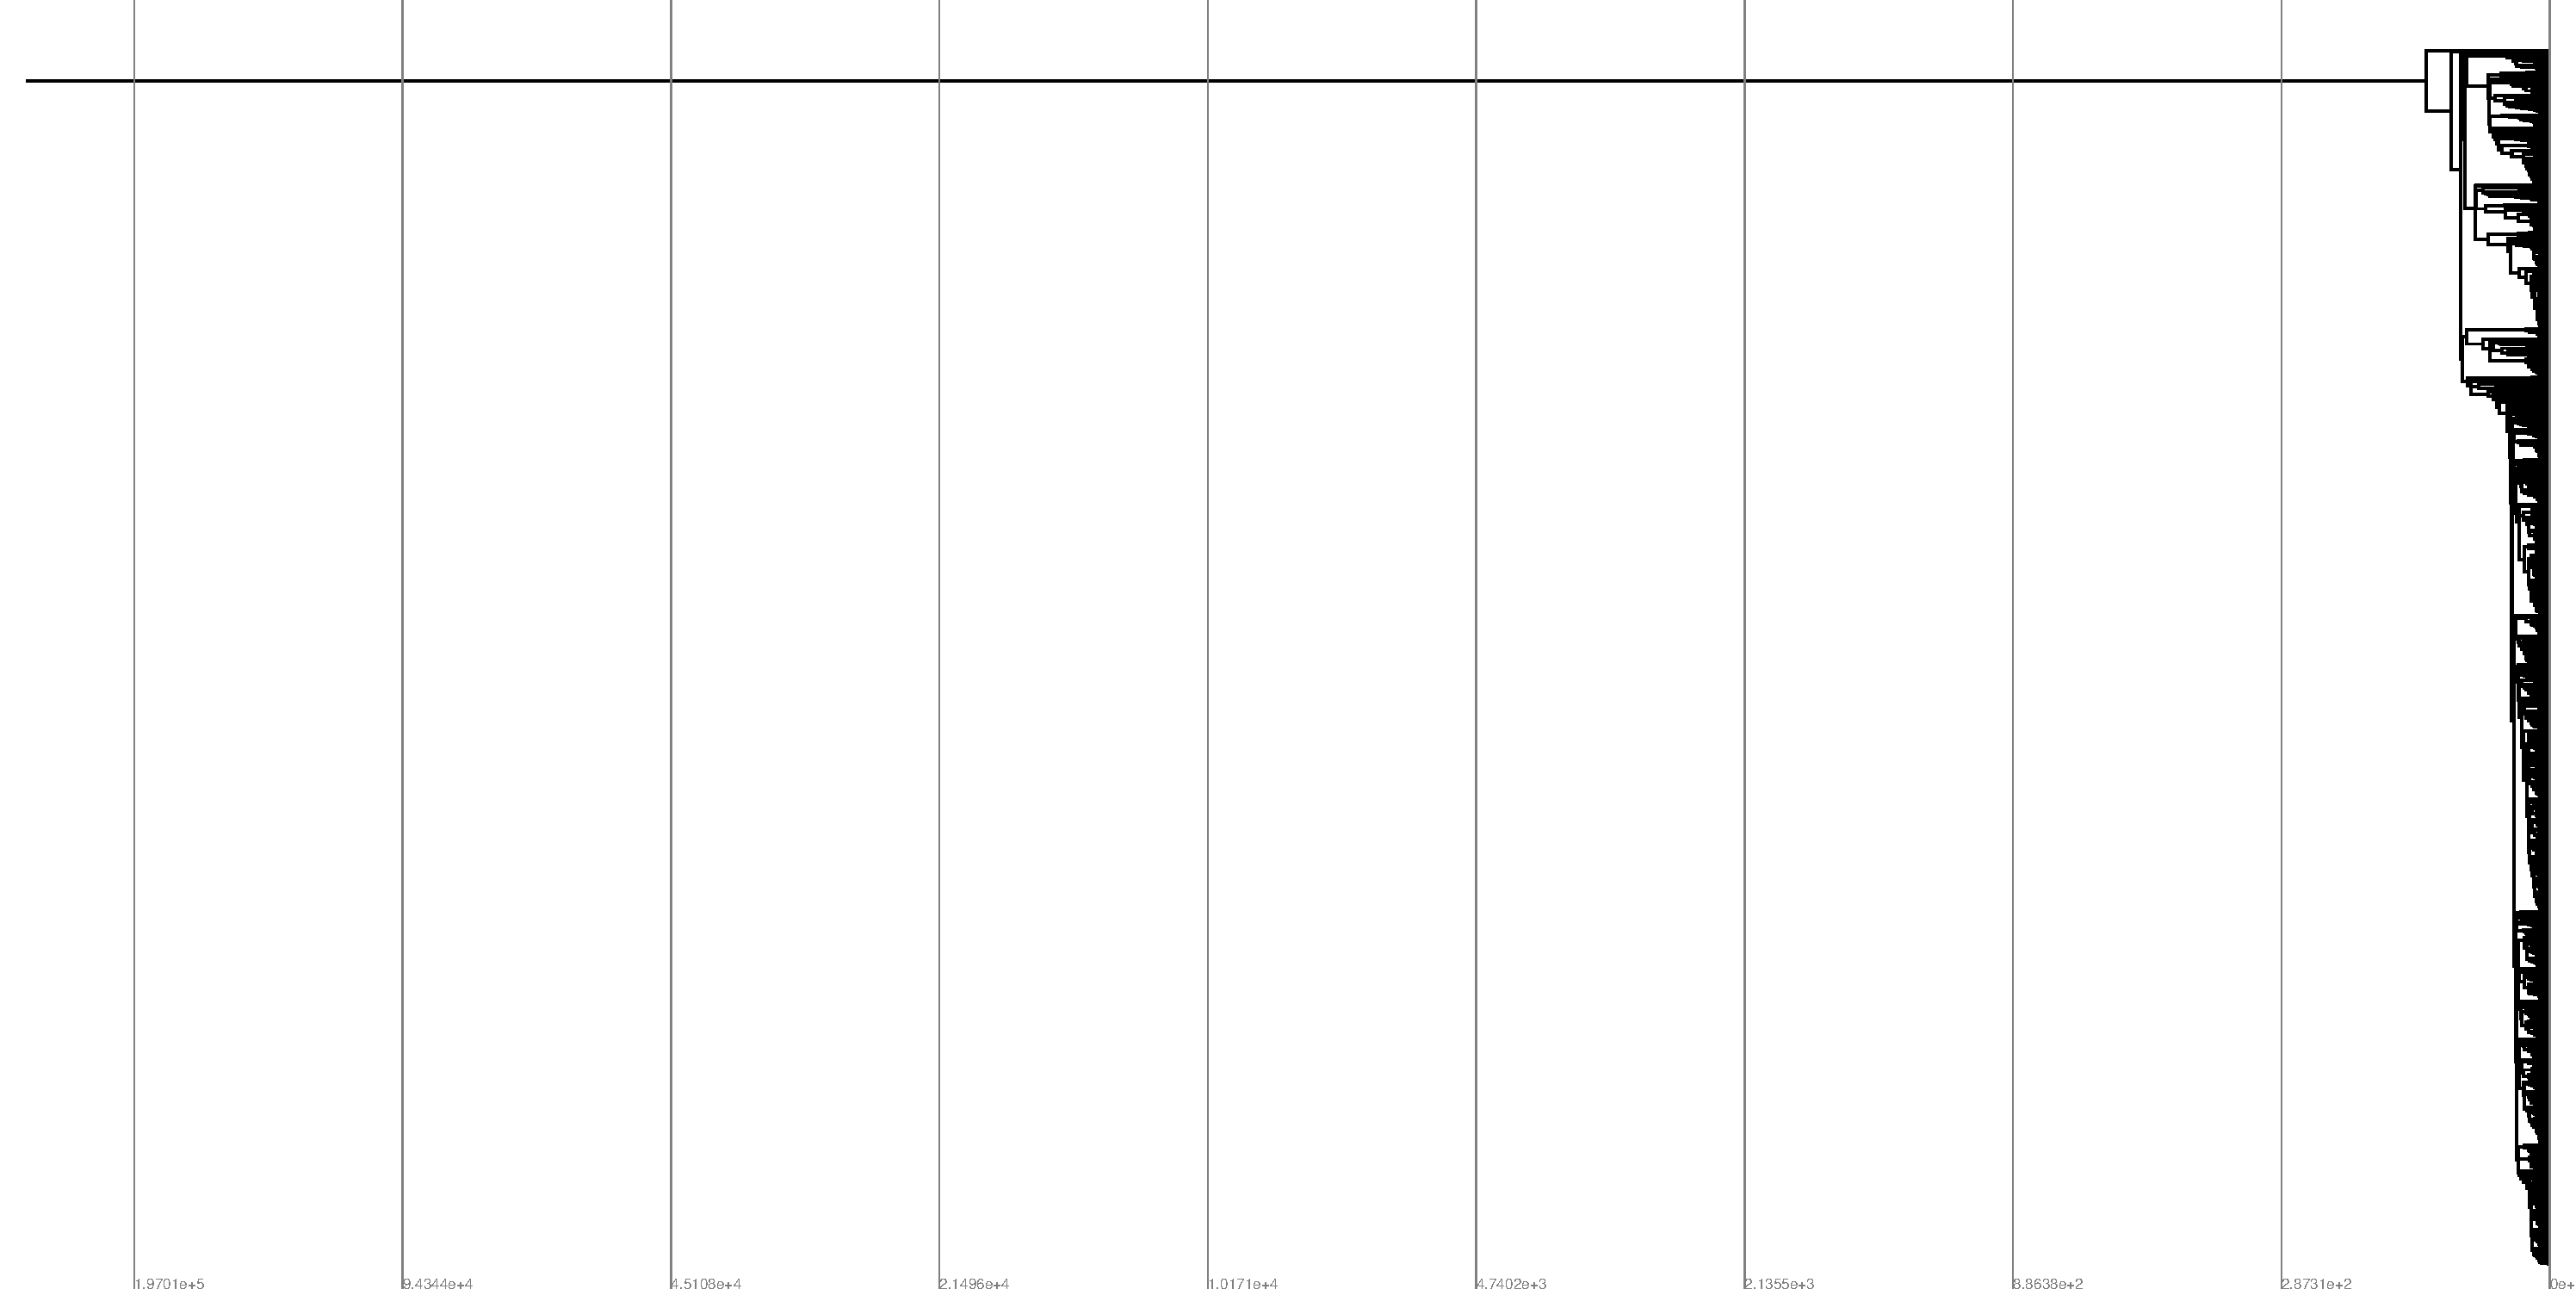
\includegraphics[height=0.12\textheight,width=\textwidth]{img/perfect-tree-phylogenies-log/epoch=7+resolution=3+treatment=8.pdf}
    % \end{noindent}
    \caption{%
      plain}
    % \label{fig:perfect-tree-phylogenies-log:TODO}
  \end{subfigure}
  \hfill
  \begin{subfigure}[b]{0.5\columnwidth}
    % \begin{noindent}
    % 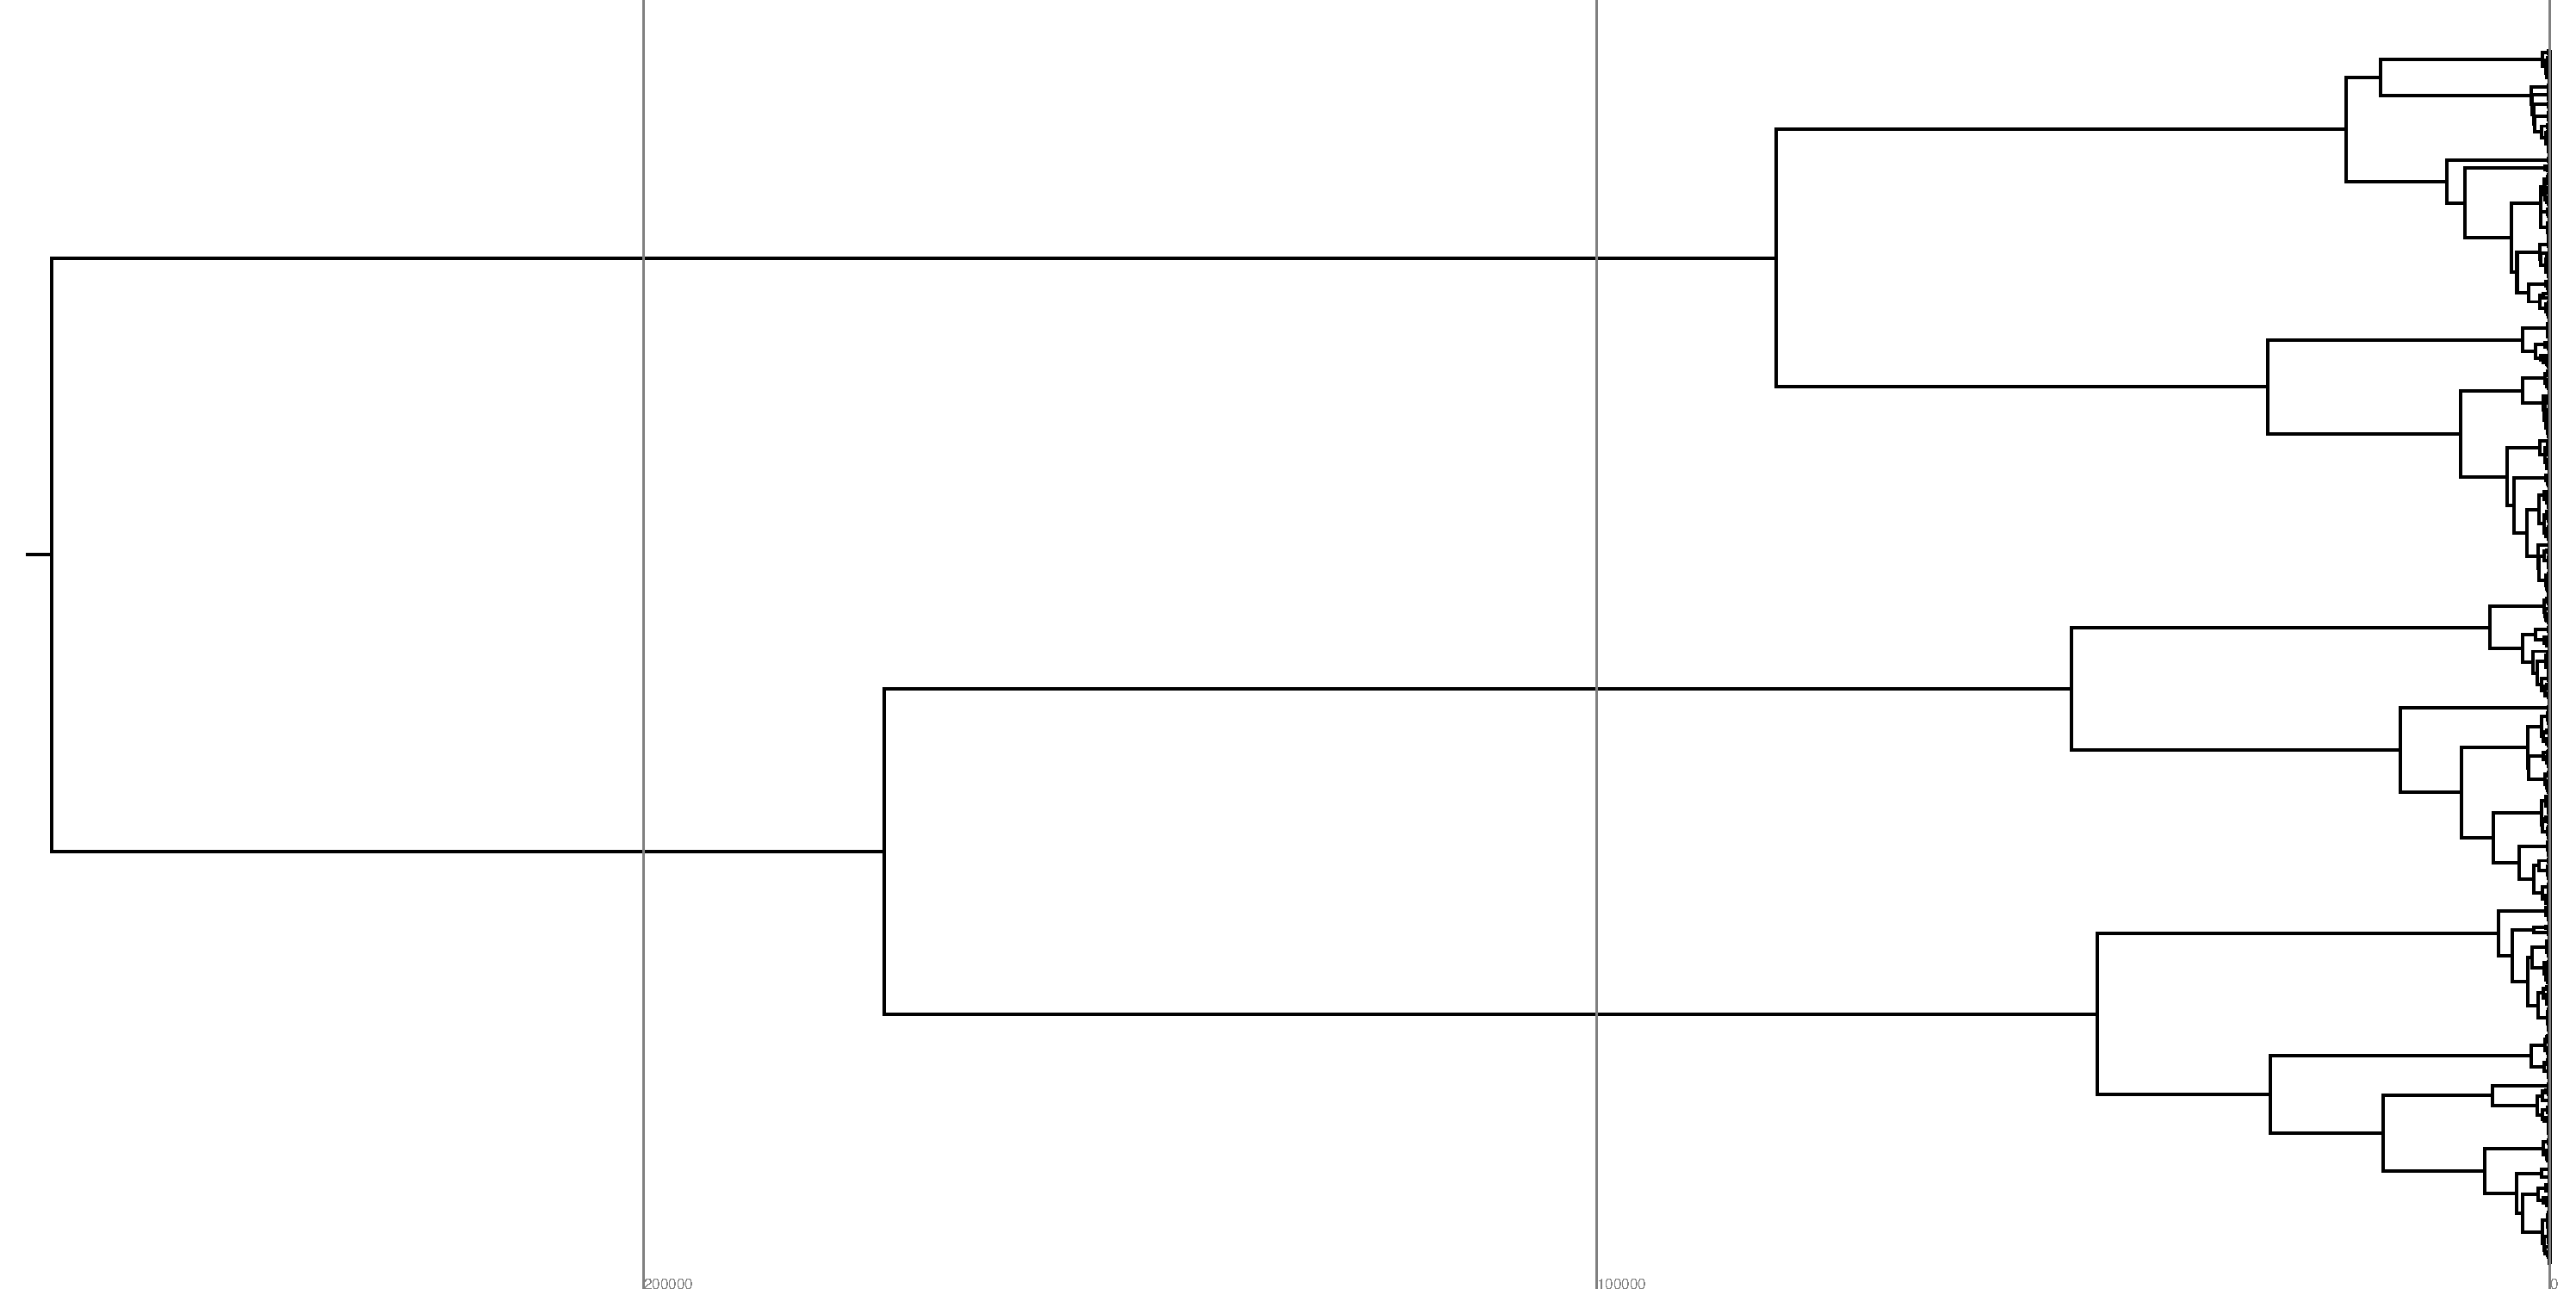
\includegraphics[height=0.12\textheight,width=\textwidth]{img/perfect-tree-phylogenies-log/epoch=7+resolution=3+treatment=6/a=collapsed-phylogeny+epoch=00007+mut_distn=np.random.standard_normal+num_generations=32768+num_islands=1024+num_niches=1+p_island_migration=0.01+p_niche_invasion=3.0517578125e-08+population_size=3276.../8+replicate=0+tournament_size=2+treatment=6+_generation=262144+_index=6+scale=nonlog+ext=.pdf}
    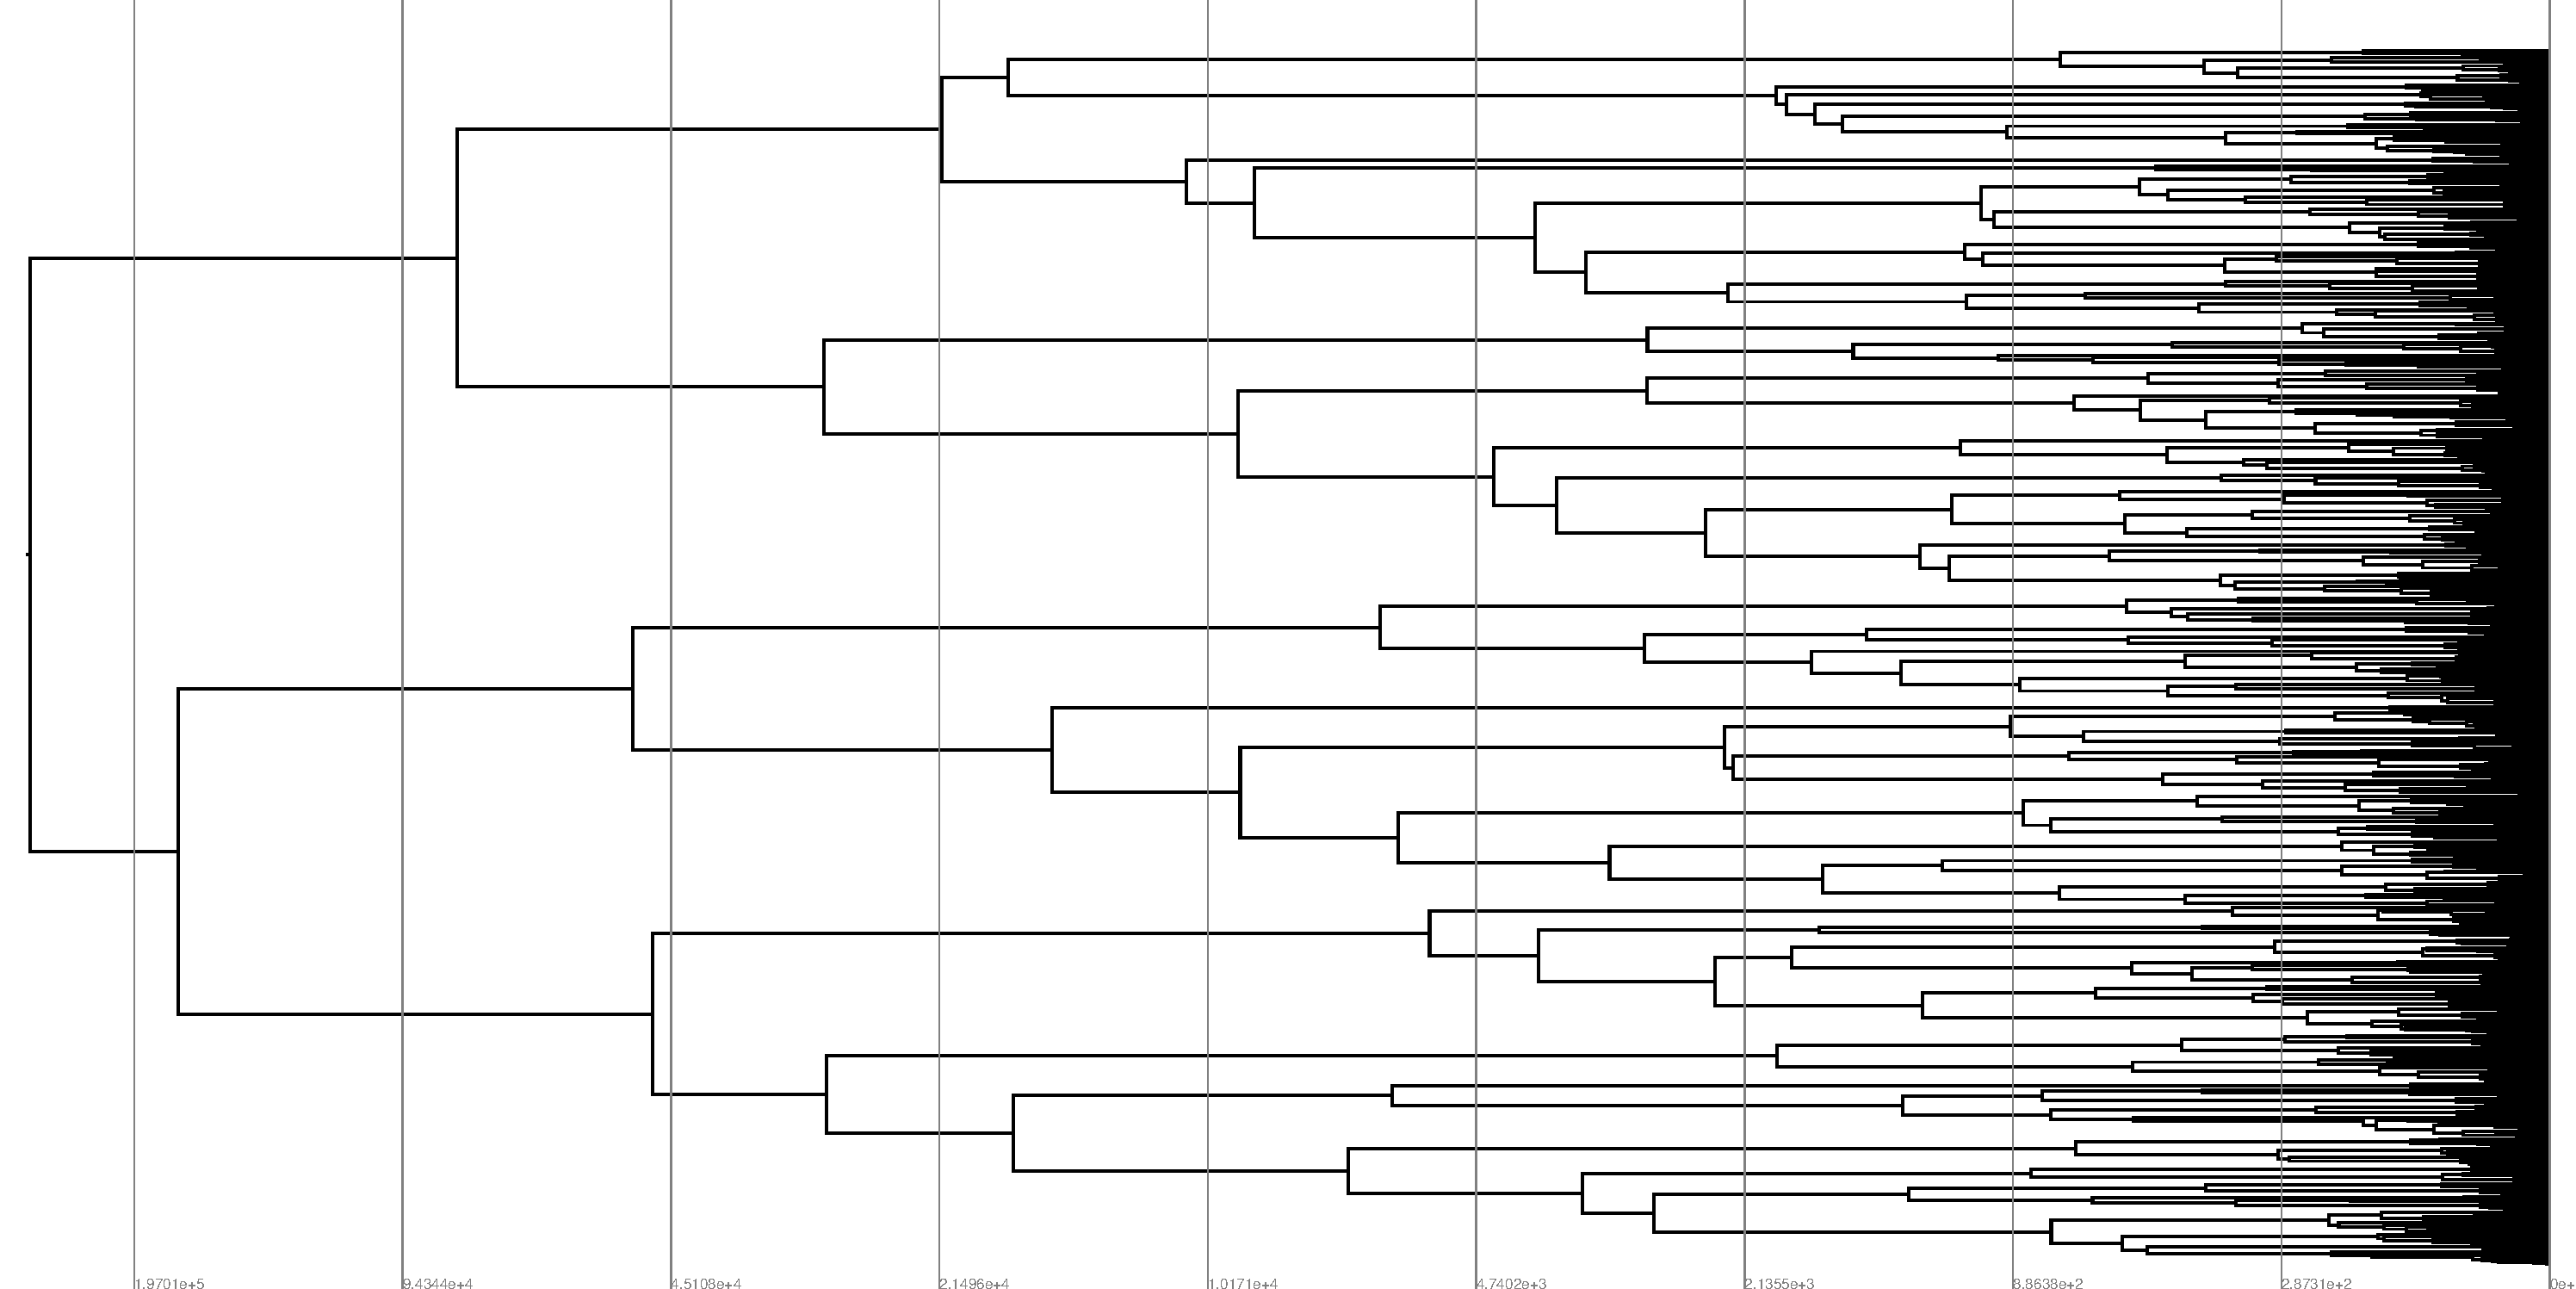
\includegraphics[height=0.12\textheight,width=\textwidth]{img/perfect-tree-phylogenies-log/epoch=7+resolution=3+treatment=6.pdf}
    % \end{noindent}
    \caption{%
      spatial structure}
    % \label{fig:perfect-tree-phylogenies-log:TODO}
  \end{subfigure}
  \hfill
  \begin{subfigure}[b]{0.5\columnwidth}
    % 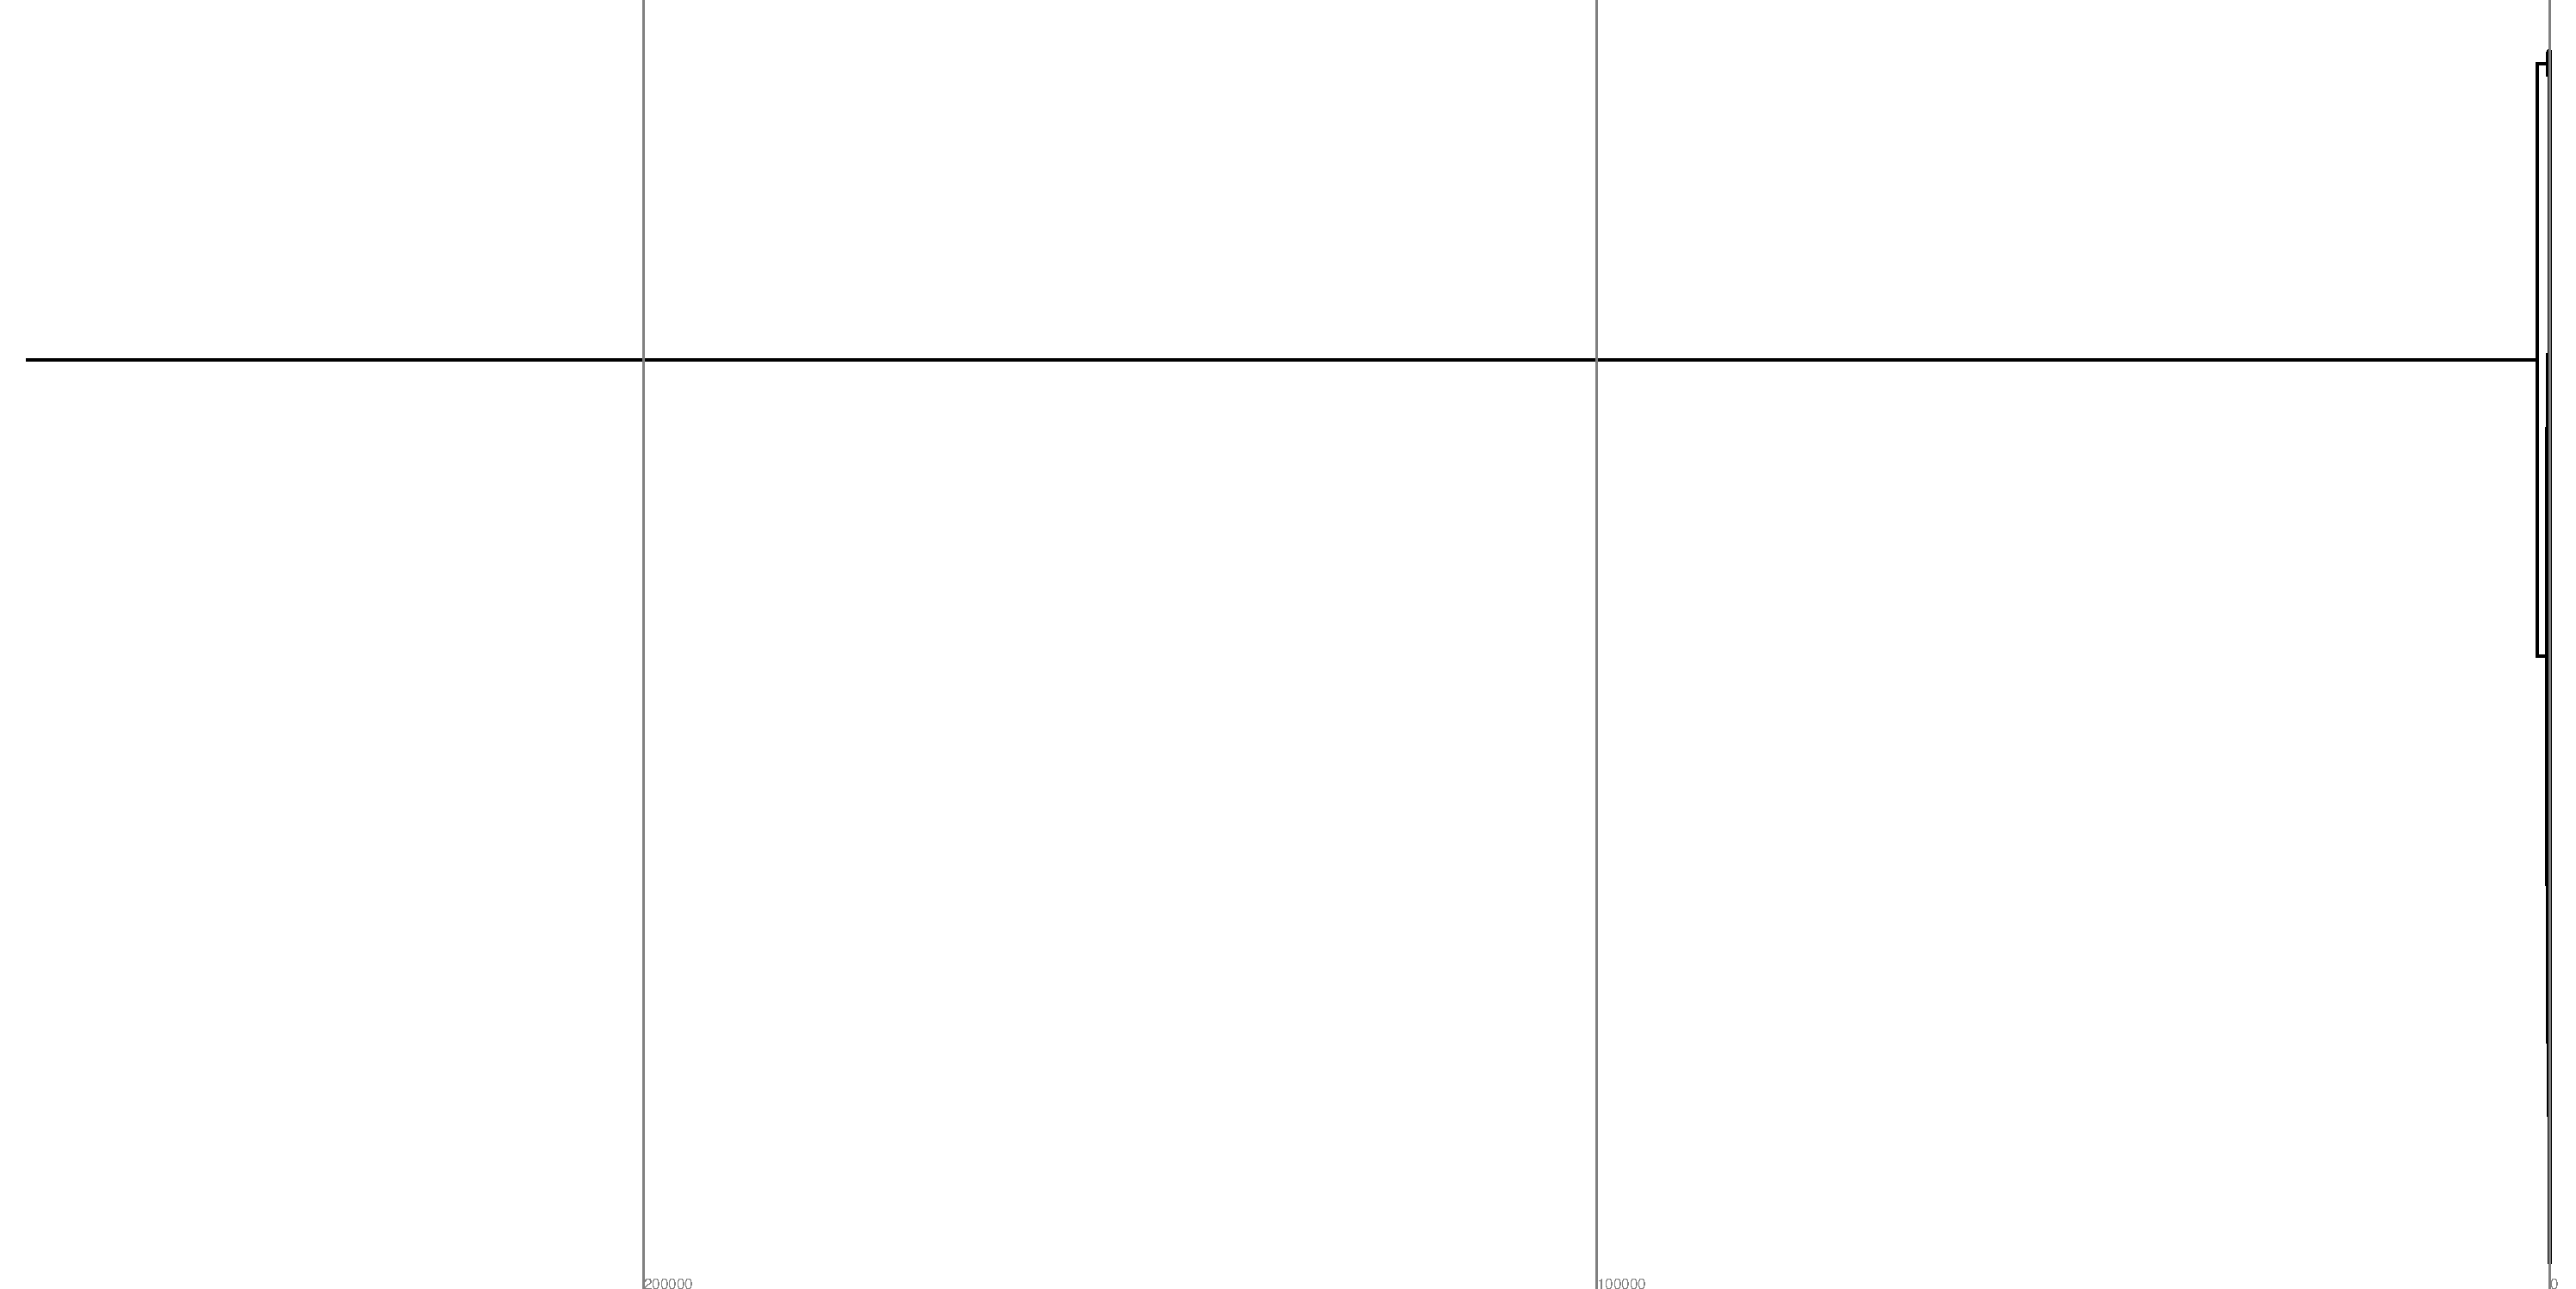
\includegraphics[height=0.12\textheight,width=\textwidth]{img/perfect-tree-phylogenies-log/epoch=7+resolution=3+treatment=26/a=collapsed-phylogeny+epoch=00007+mut_distn=np.random.standard_normal+num_generations=32768+num_islands=1+num_niches=4+p_island_migration=0.01+p_niche_invasion=3.0517578125e-06+population_size=32768+r.../eplicate=0+tournament_size=2+treatment=26+_generation=262144+_index=26+scale=nonlog+ext=.pdf}
    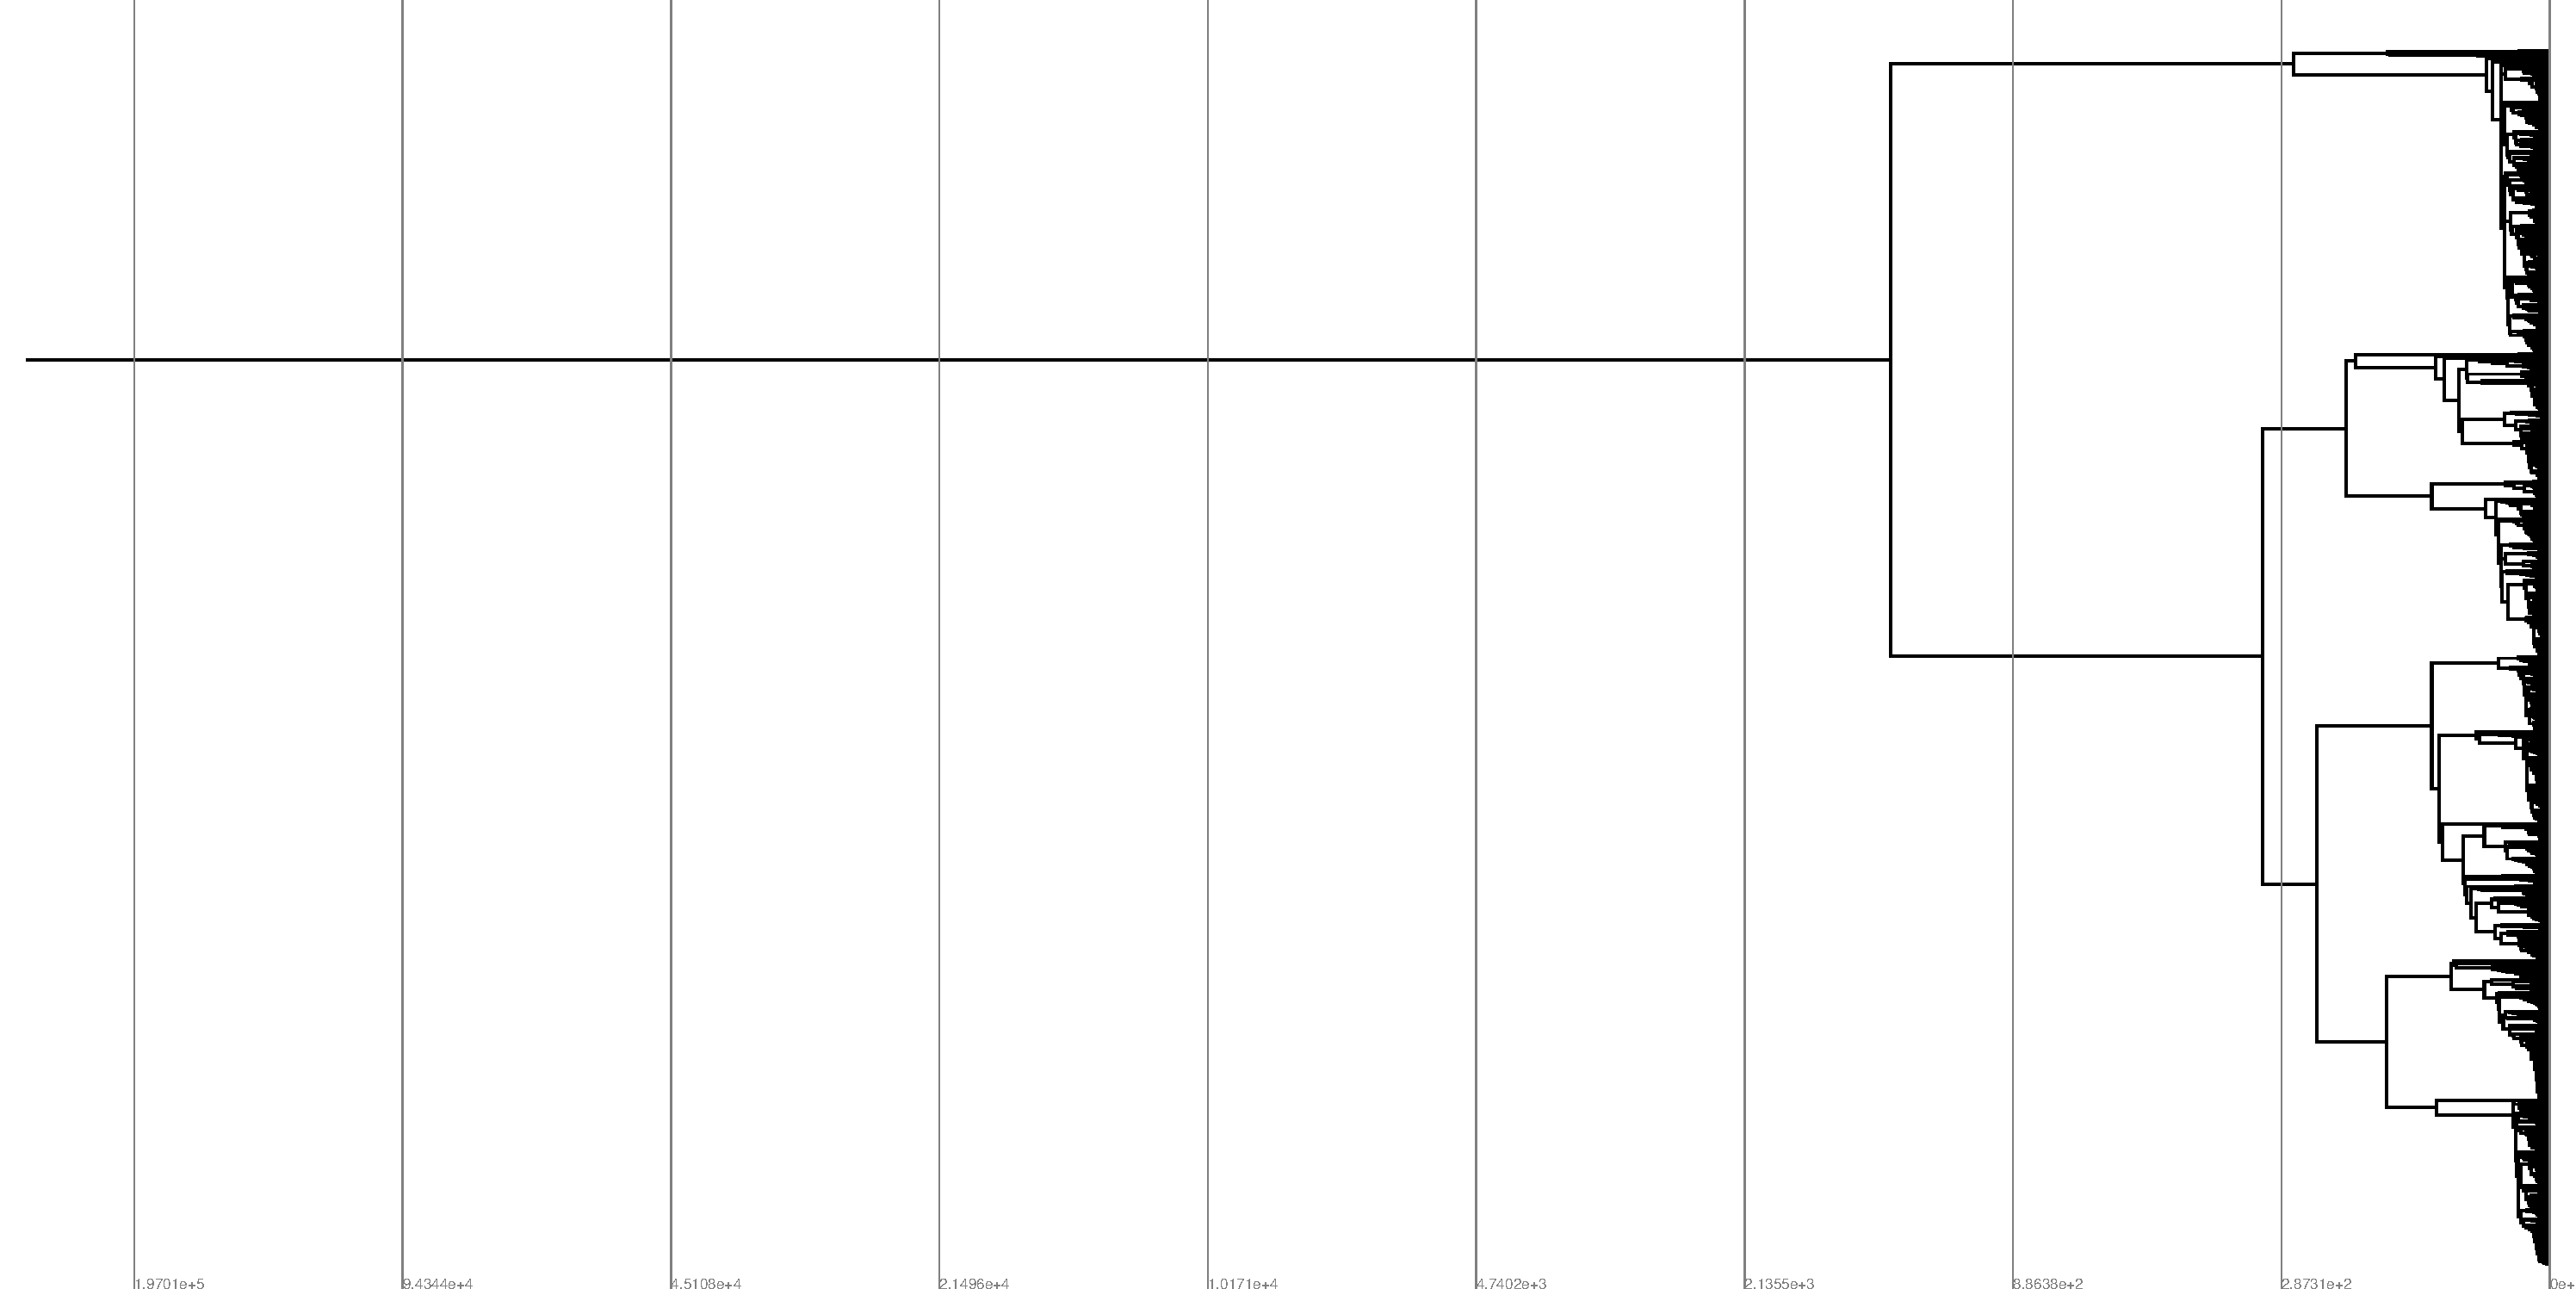
\includegraphics[height=0.12\textheight,width=\textwidth]{img/perfect-tree-phylogenies-log/epoch=7+resolution=3+treatment=26.pdf}
    % \end{noindent}
    \caption{%
      weak 4 niche ecology}
    % \label{fig:perfect-tree-phylogenies-log:TODO}
  \end{subfigure}
  \hfill
  \begin{subfigure}[b]{0.5\columnwidth}
    % \begin{noindent}
      % 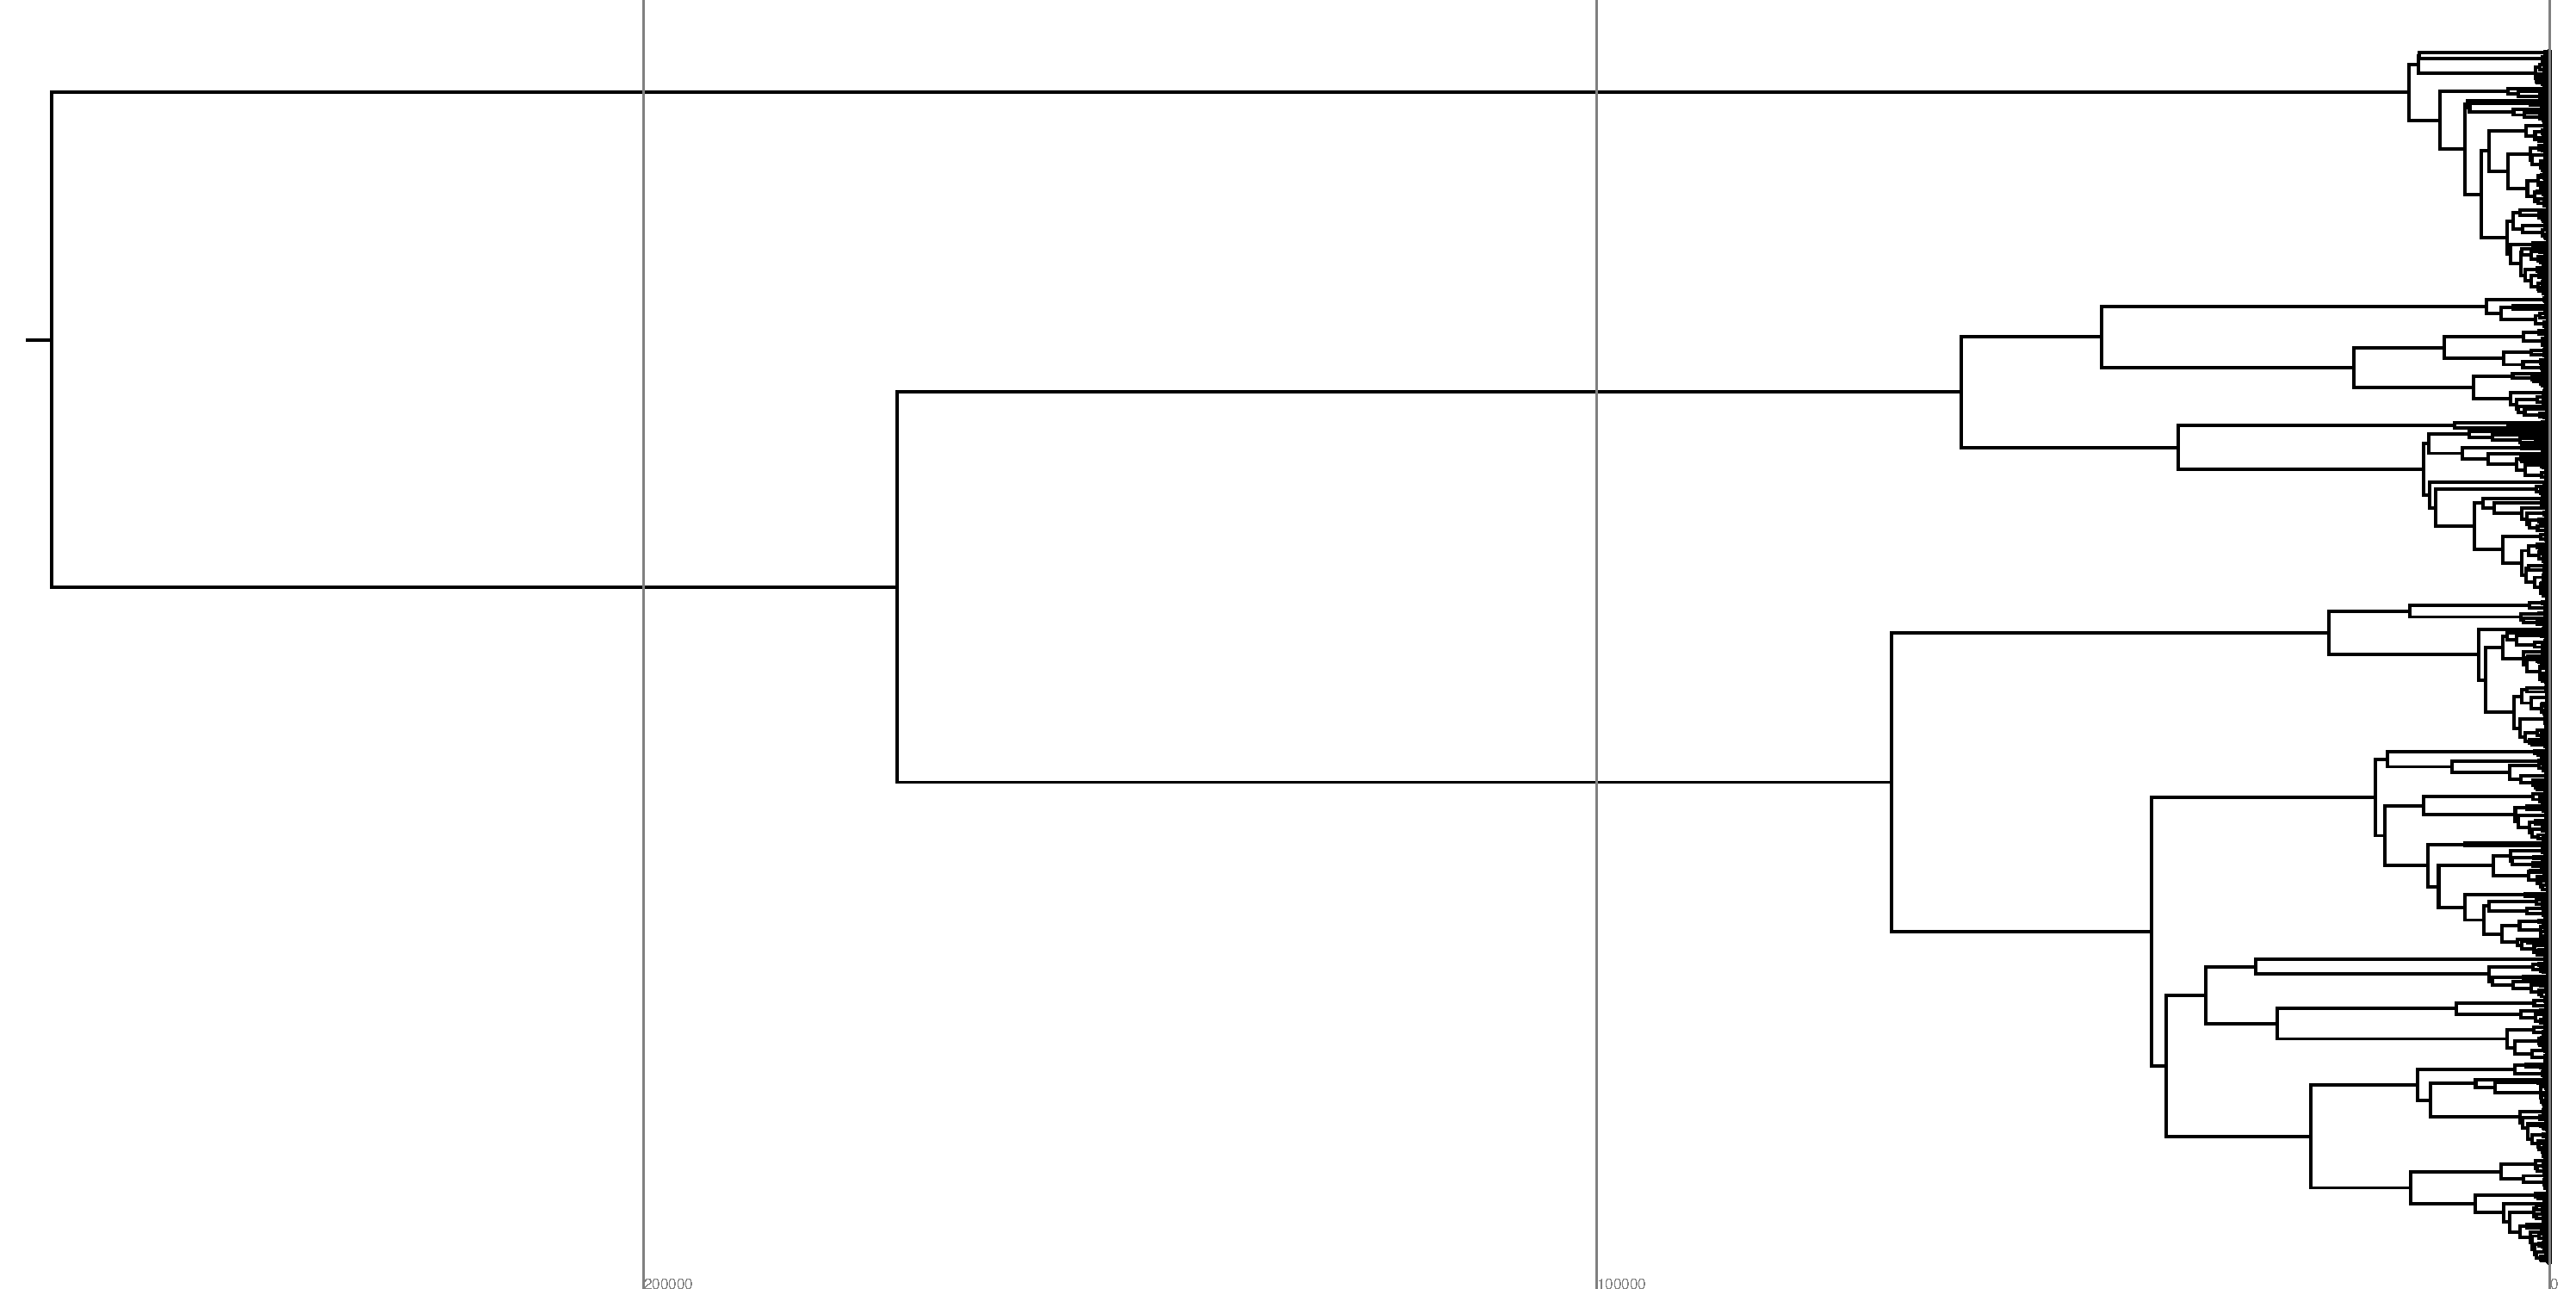
\includegraphics[height=0.12\textheight,width=\textwidth]{img/perfect-tree-phylogenies-log/epoch=7+resolution=3+treatment=24/a=collapsed-phylogeny+epoch=00007+mut_distn=np.random.standard_normal+num_generations=32768+num_islands=1024+num_niches=4+p_island_migration=0.01+p_niche_invasion=3.0517578125e-06+population_size=3276.../8+replicate=0+tournament_size=2+treatment=24+_generation=262144+_index=24+scale=nonlog+ext=.pdf}    % \end{noindent}
      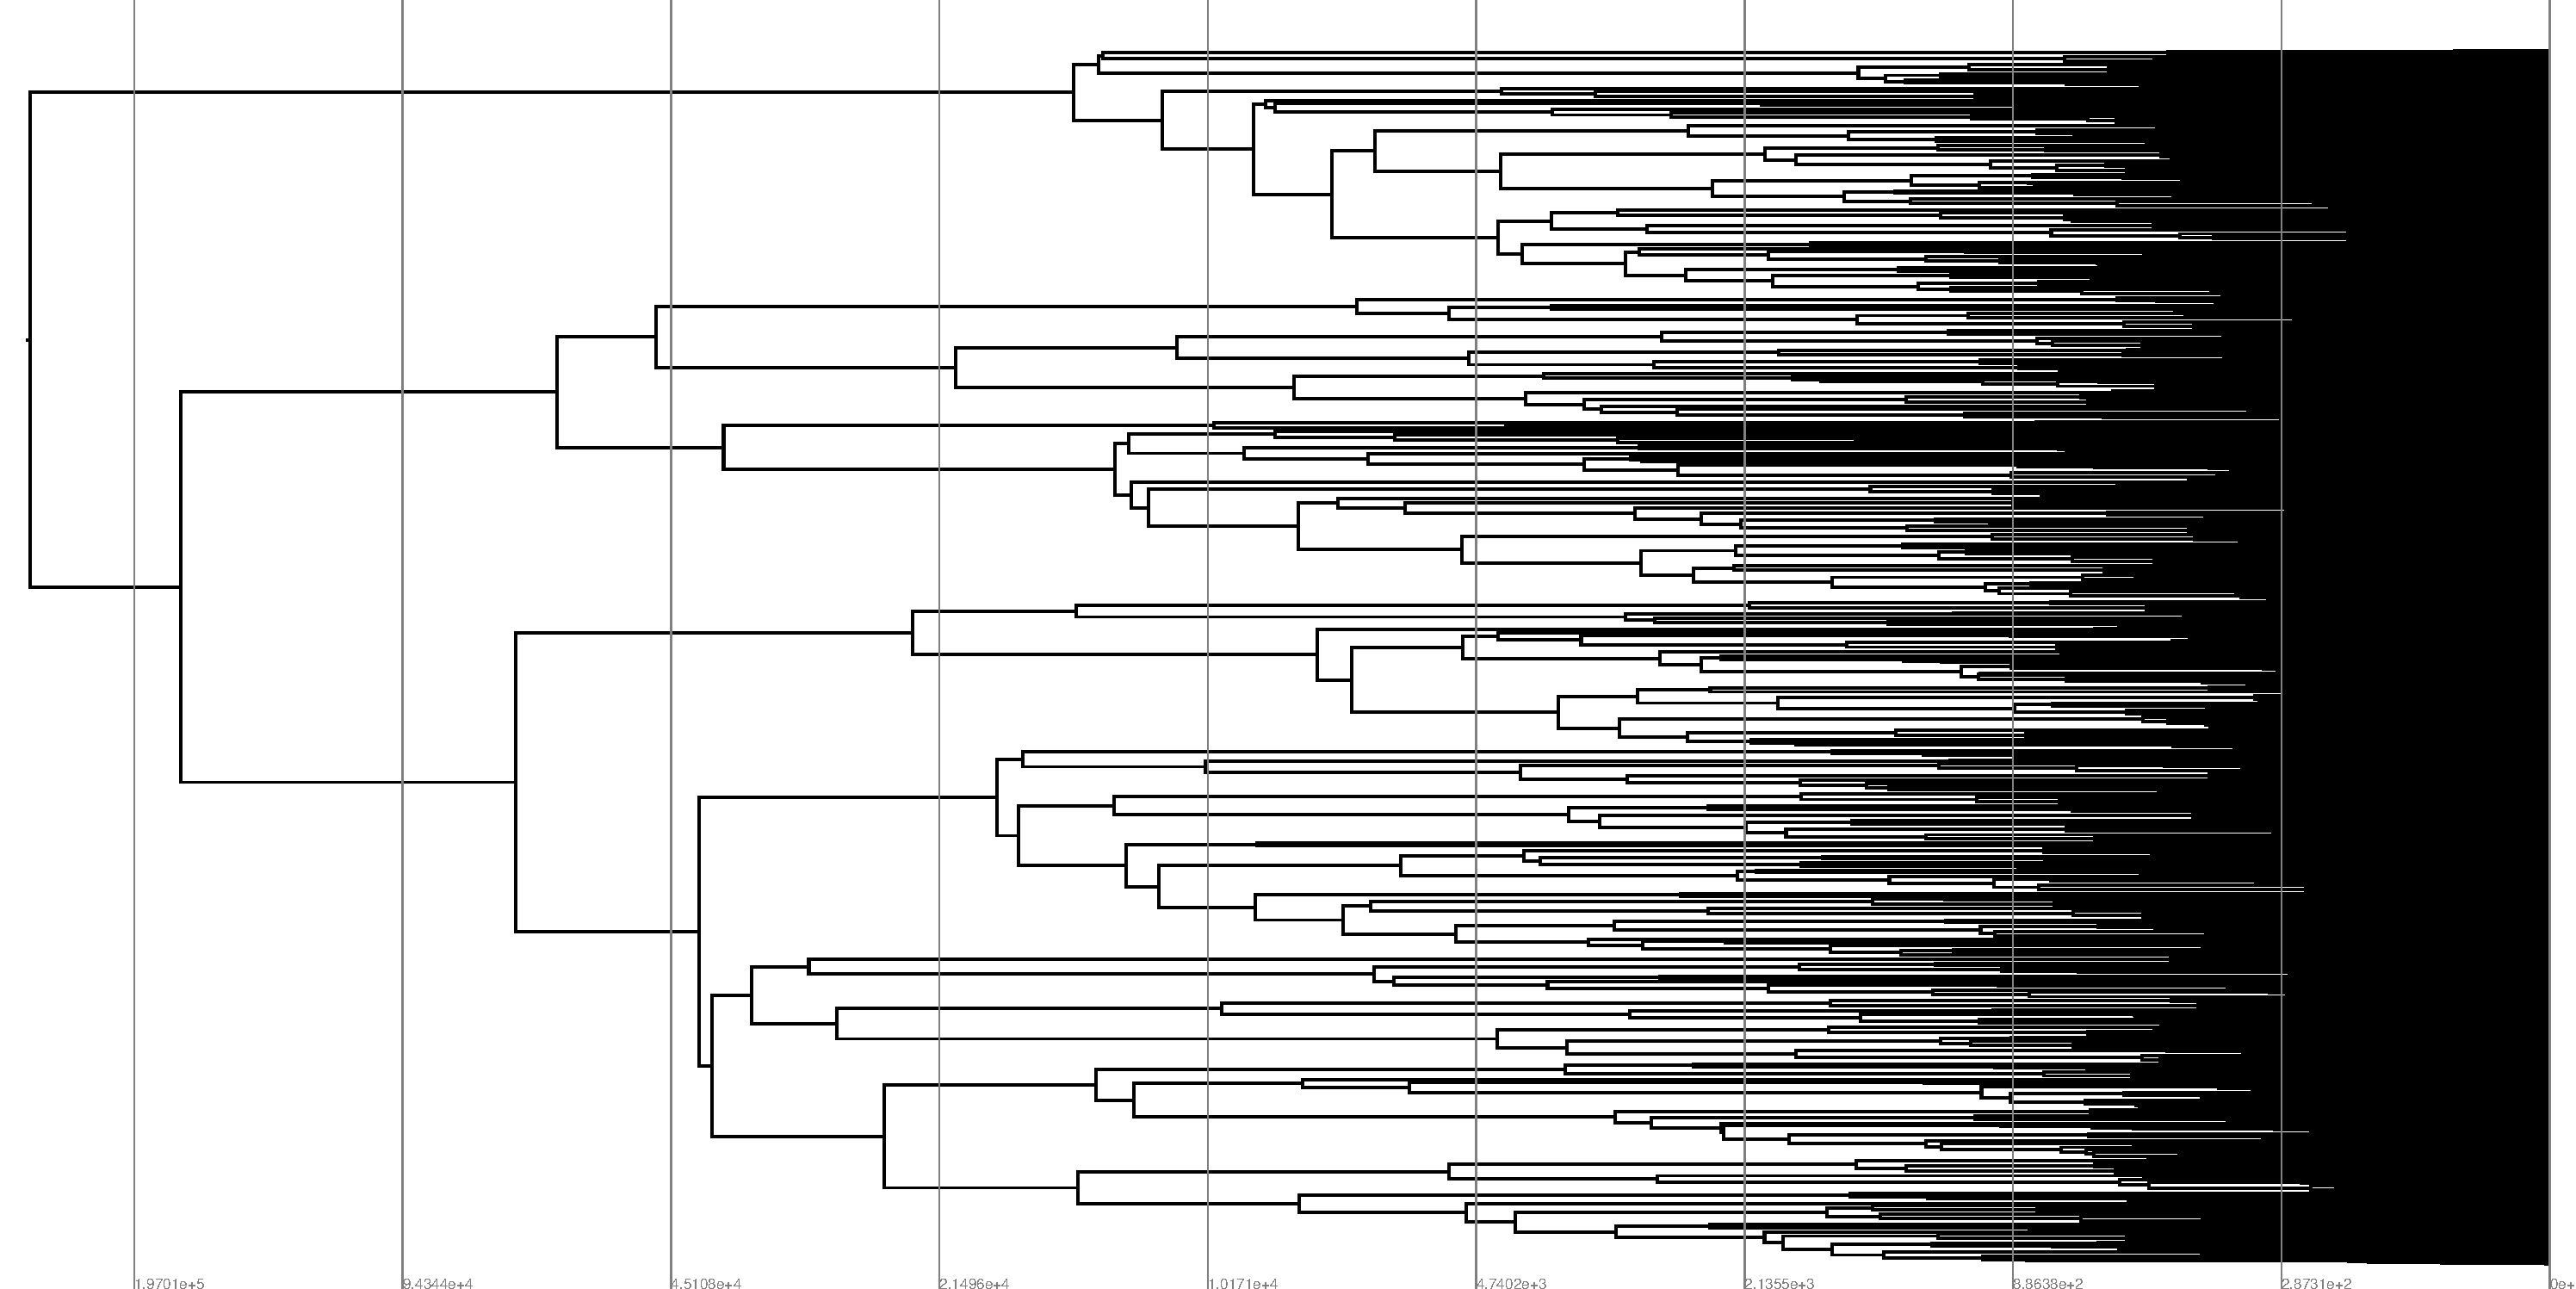
\includegraphics[height=0.12\textheight,width=\textwidth]{img/perfect-tree-phylogenies-log/epoch=7+resolution=3+treatment=24.pdf}    % \end{noindent}
    \caption{%
      weak 4 niche ecology with spatial structure }
    % \label{fig:perfect-tree-phylogenies-log:TODO}
  \end{subfigure}
  \hfill
  \begin{subfigure}[b]{0.5\columnwidth}
    % 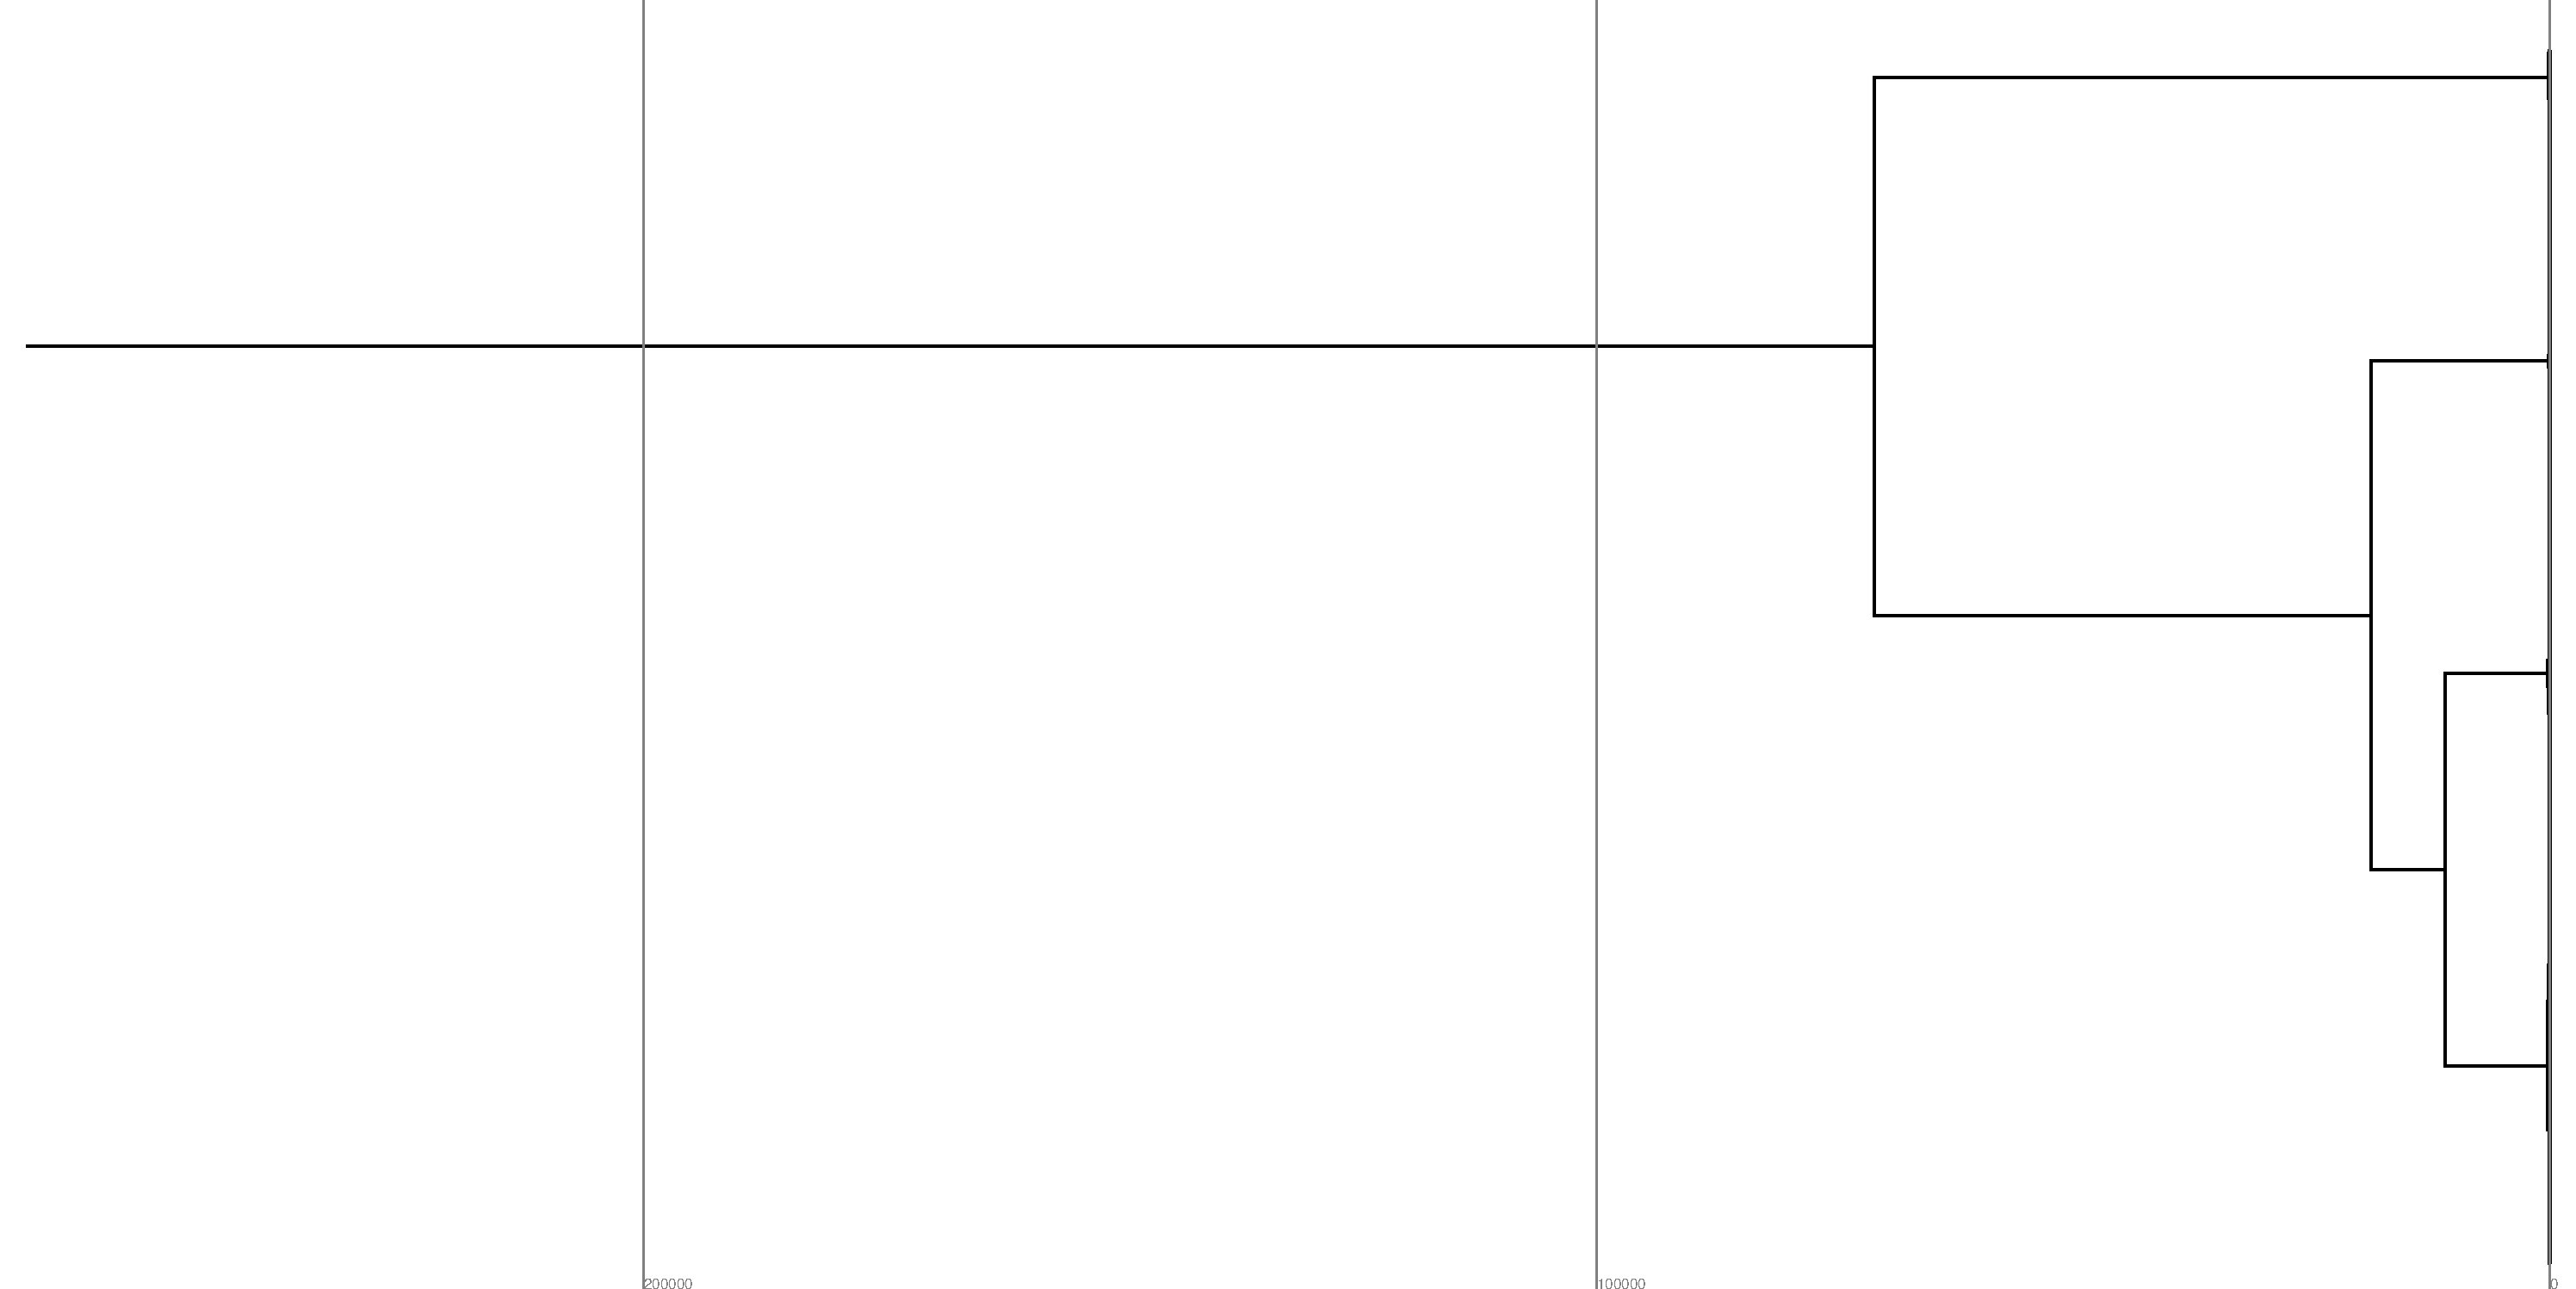
\includegraphics[height=0.12\textheight,width=\textwidth]{img/perfect-tree-phylogenies-log/epoch=7+resolution=3+treatment=10/a=collapsed-phylogeny+epoch=00007+mut_distn=np.random.standard_normal+num_generations=32768+num_islands=1+num_niches=4+p_island_migration=0.01+p_niche_invasion=3.0517578125e-08+population_size=32768+r.../eplicate=0+tournament_size=2+treatment=10+_generation=262144+_index=10+scale=nonlog+ext=.pdf}
    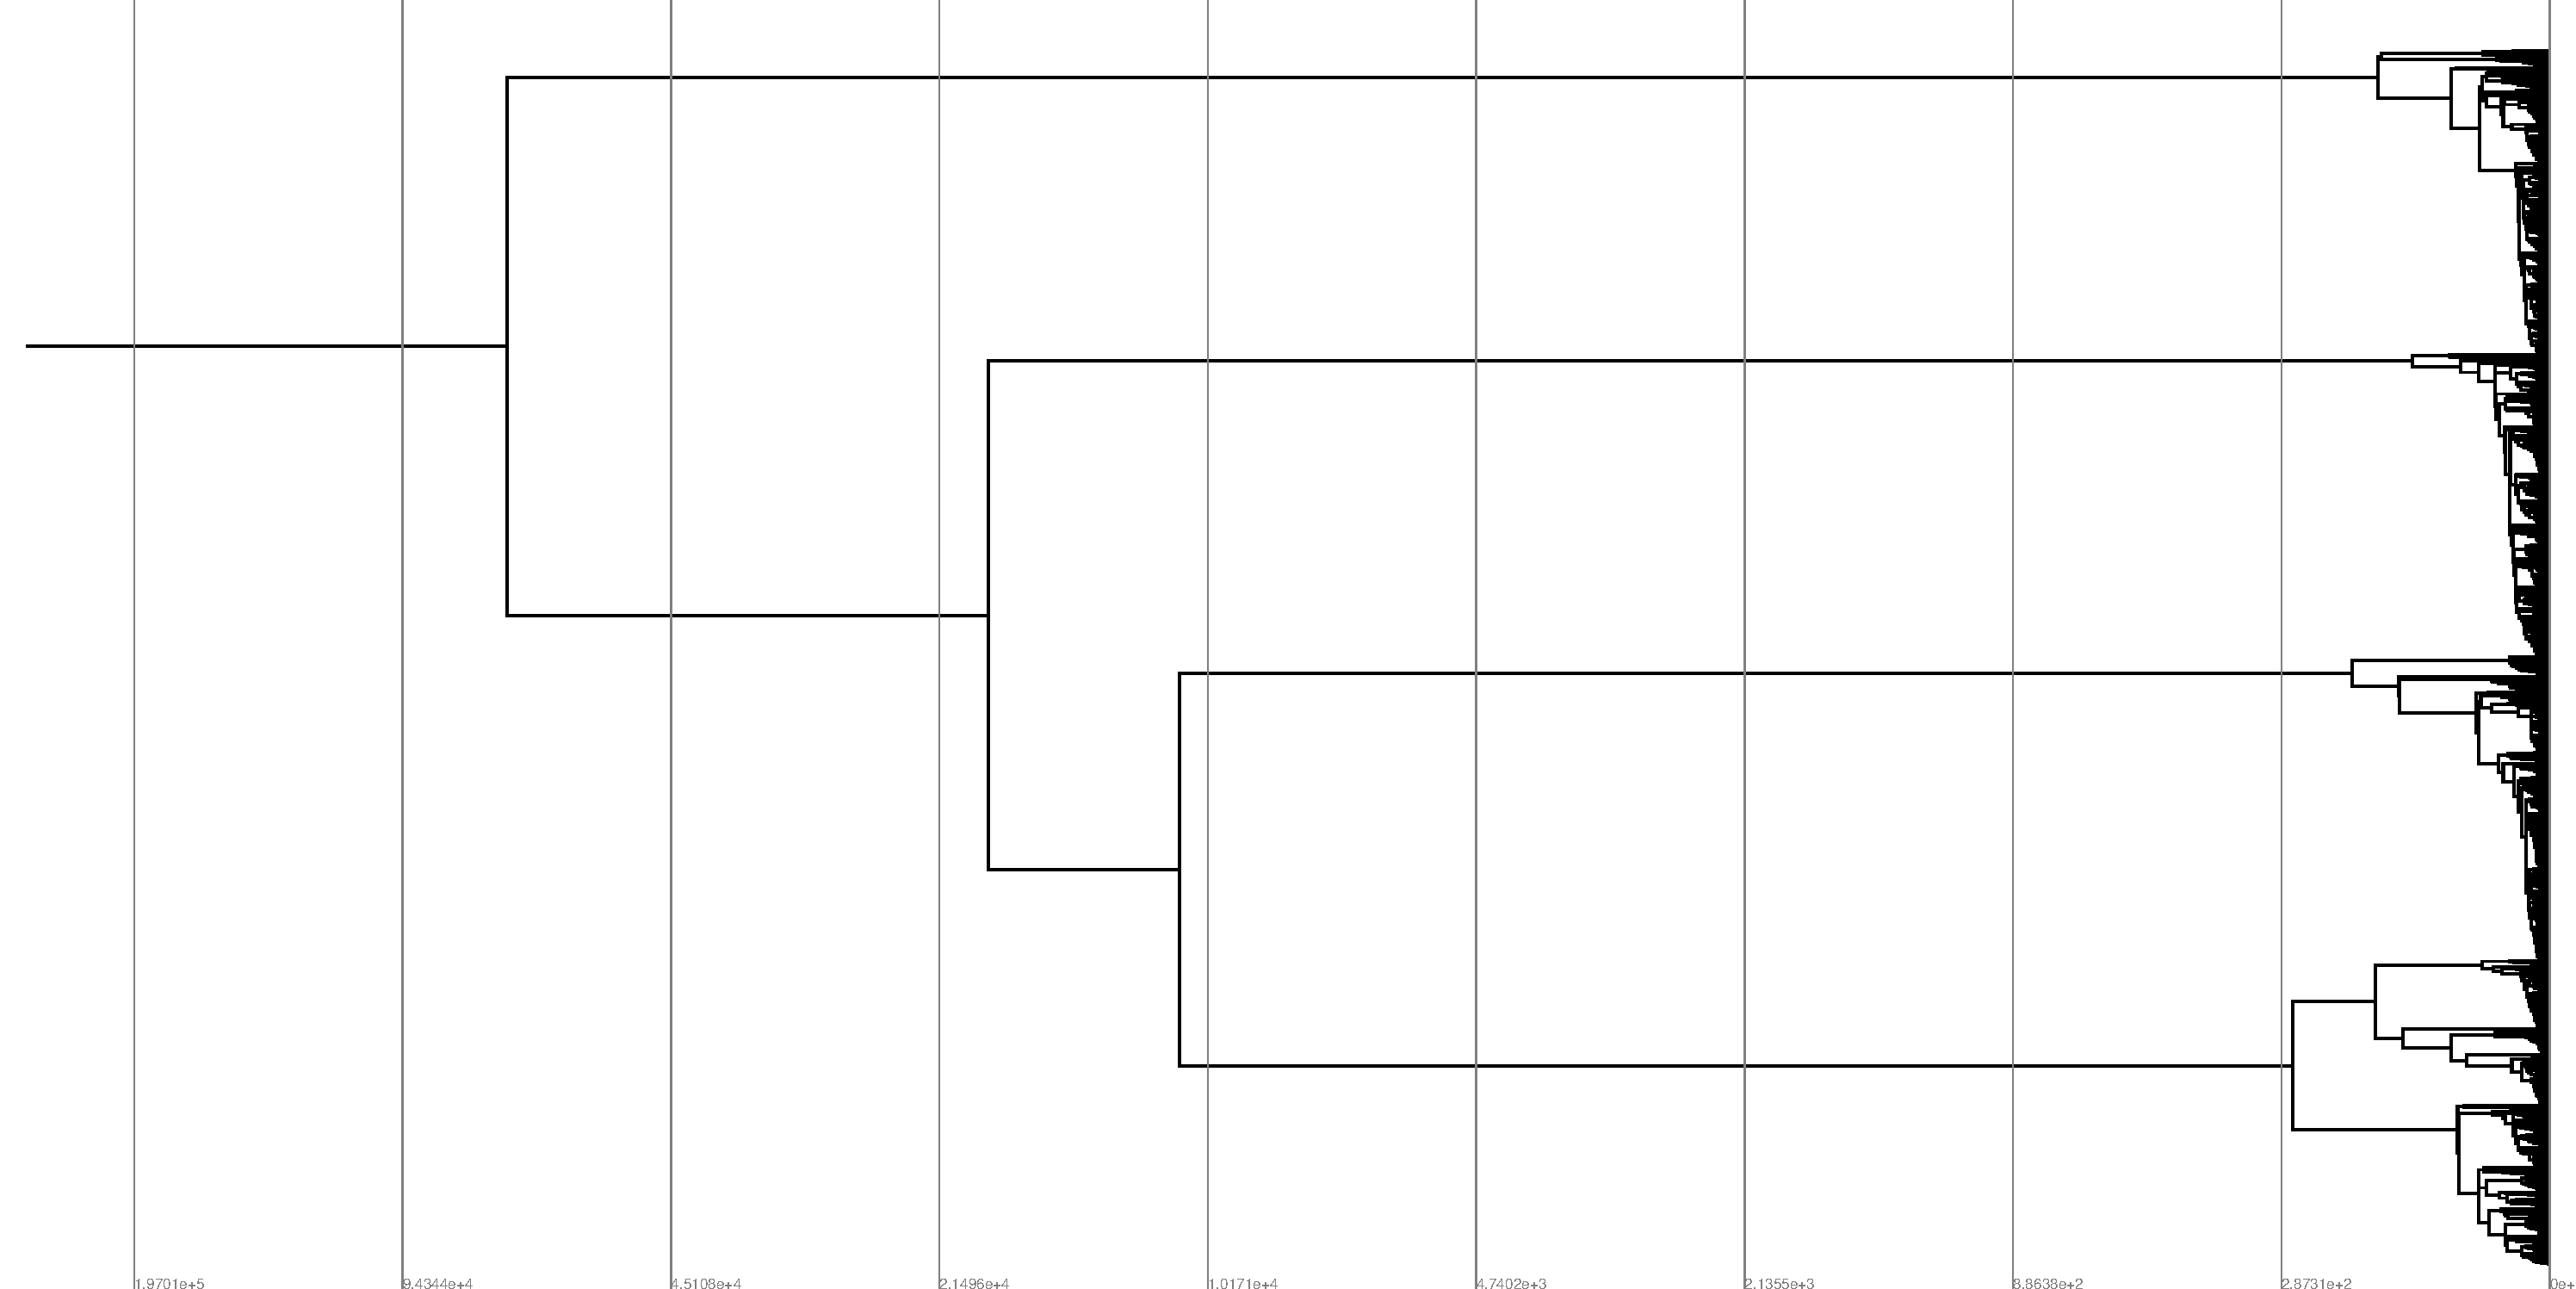
\includegraphics[height=0.12\textheight,width=\textwidth]{img/perfect-tree-phylogenies-log/epoch=7+resolution=3+treatment=10.pdf}
    % \end{noindent}
    \caption{%
      4 niche ecology}
    % \label{fig:perfect-tree-phylogenies-log:TODO}
  \end{subfigure}
  \hfill
  \begin{subfigure}[b]{0.5\columnwidth}
    % \begin{noindent}
    % 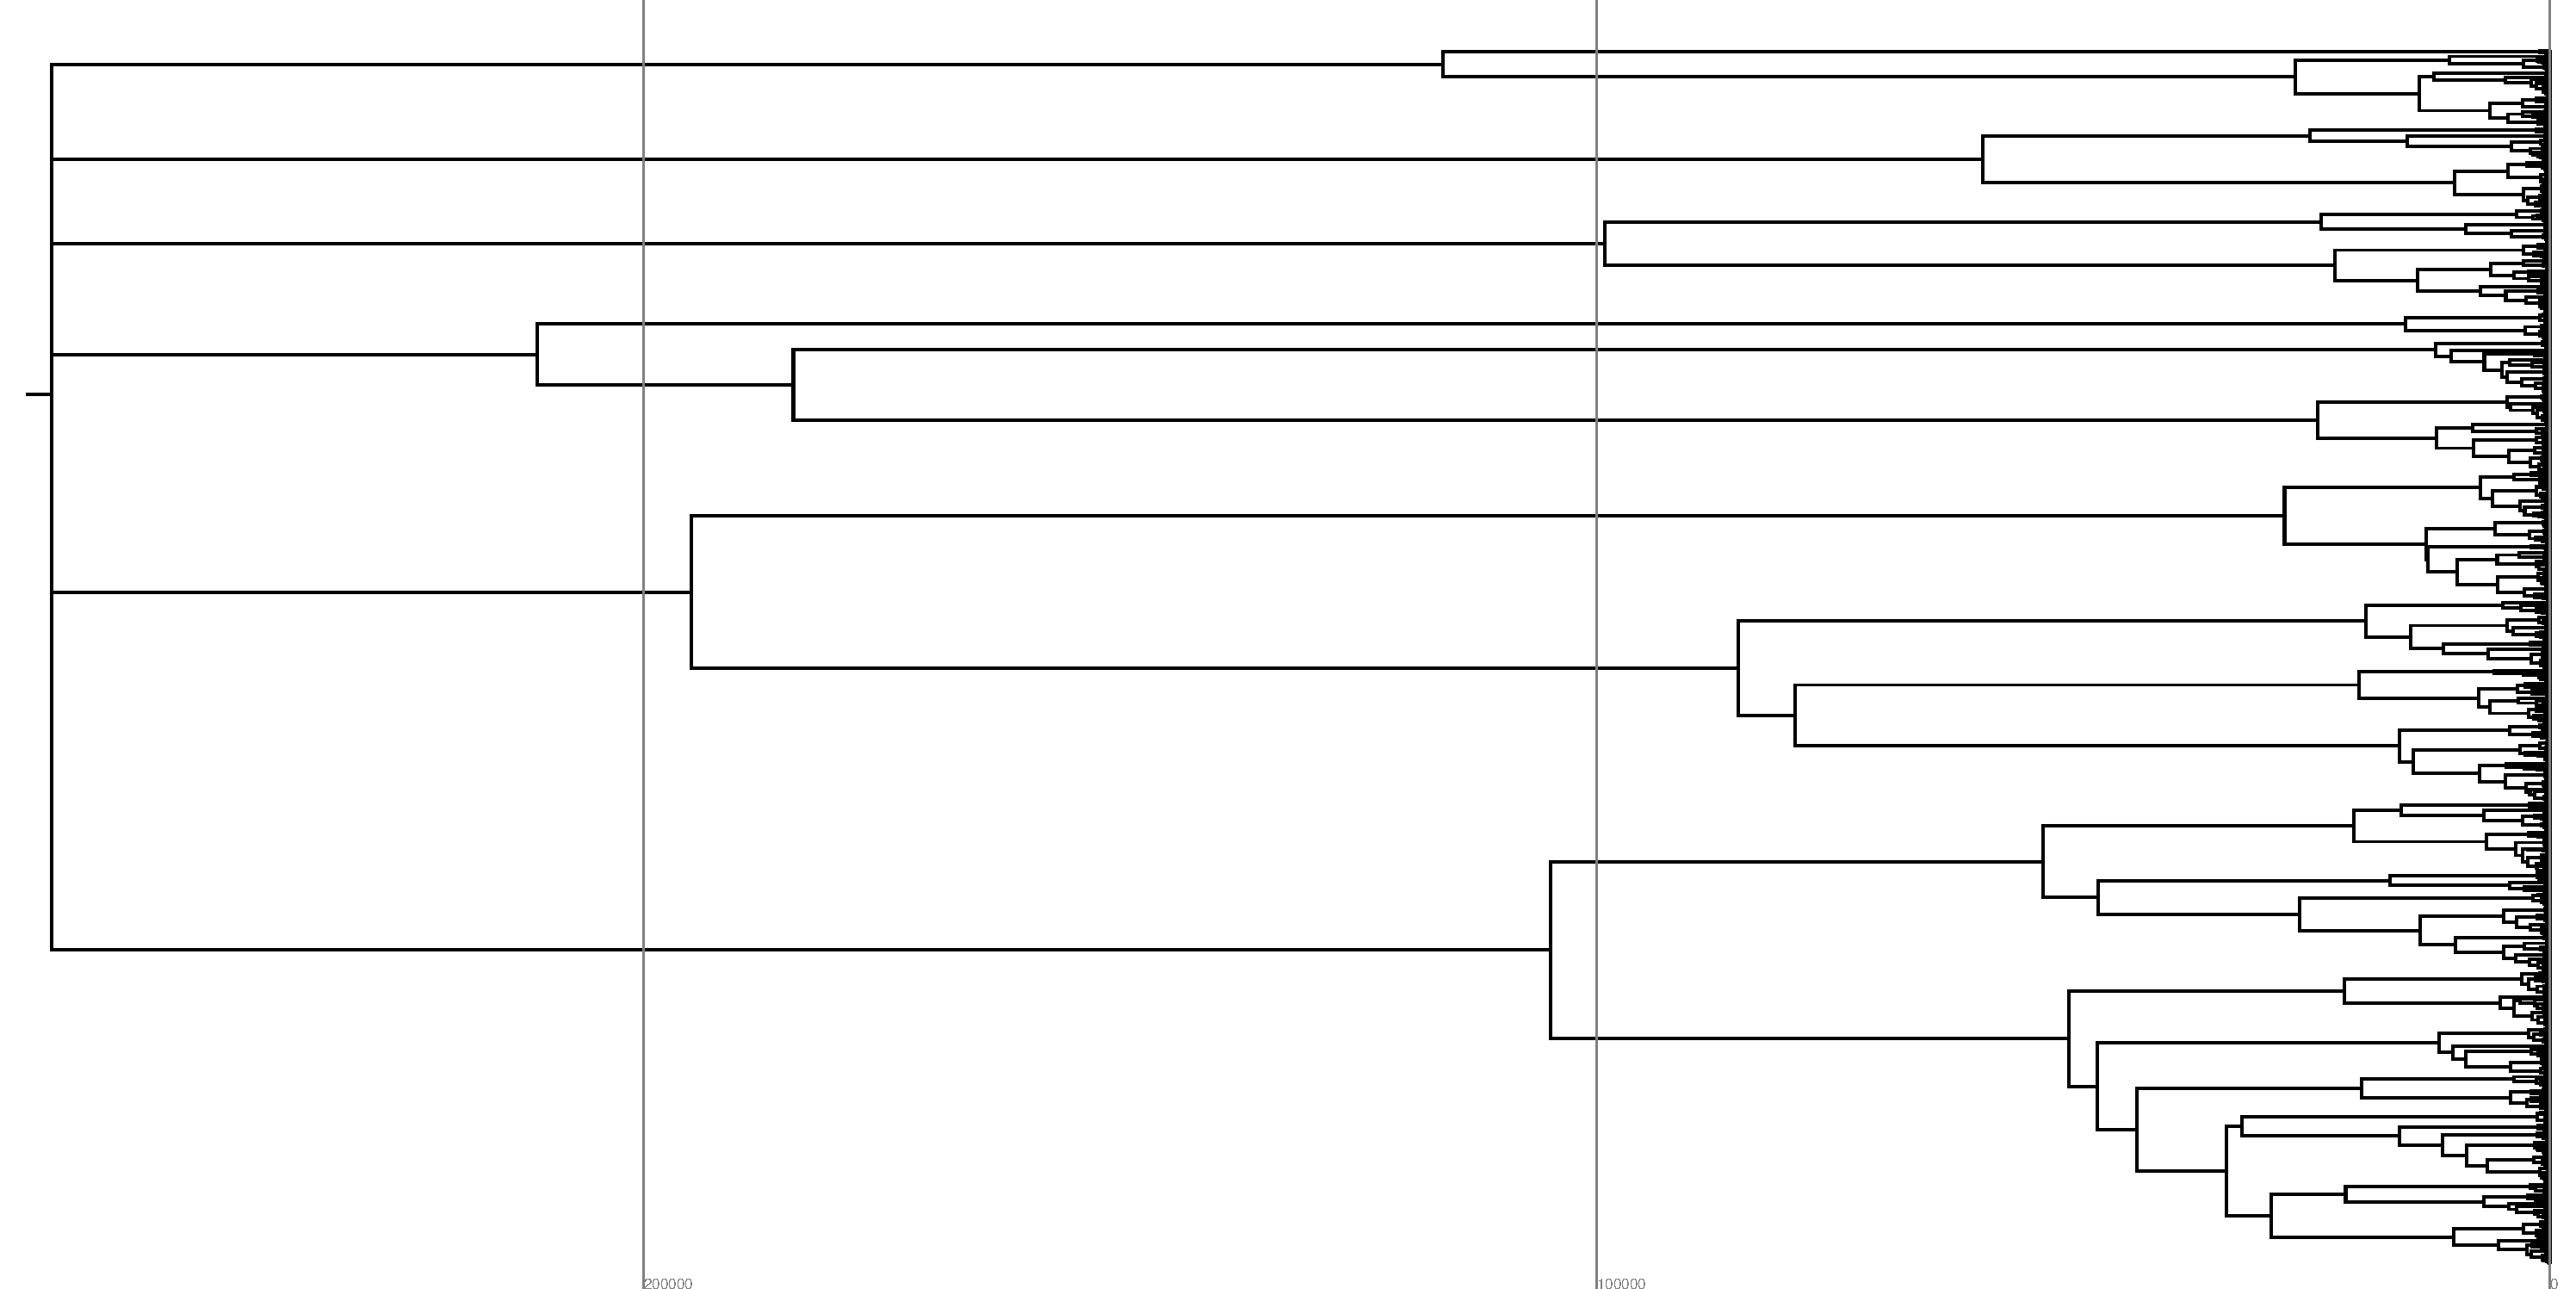
\includegraphics[height=0.12\textheight,width=\textwidth]{img/perfect-tree-phylogenies-log/epoch=7+resolution=3+treatment=22/a=collapsed-phylogeny+epoch=00007+mut_distn=np.random.standard_normal+num_generations=32768+num_islands=1024+num_niches=4+p_island_migration=0.01+p_niche_invasion=3.0517578125e-08+population_size=3276.../8+replicate=0+tournament_size=2+treatment=22+_generation=262144+_index=22+scale=nonlog+ext=.pdf}
    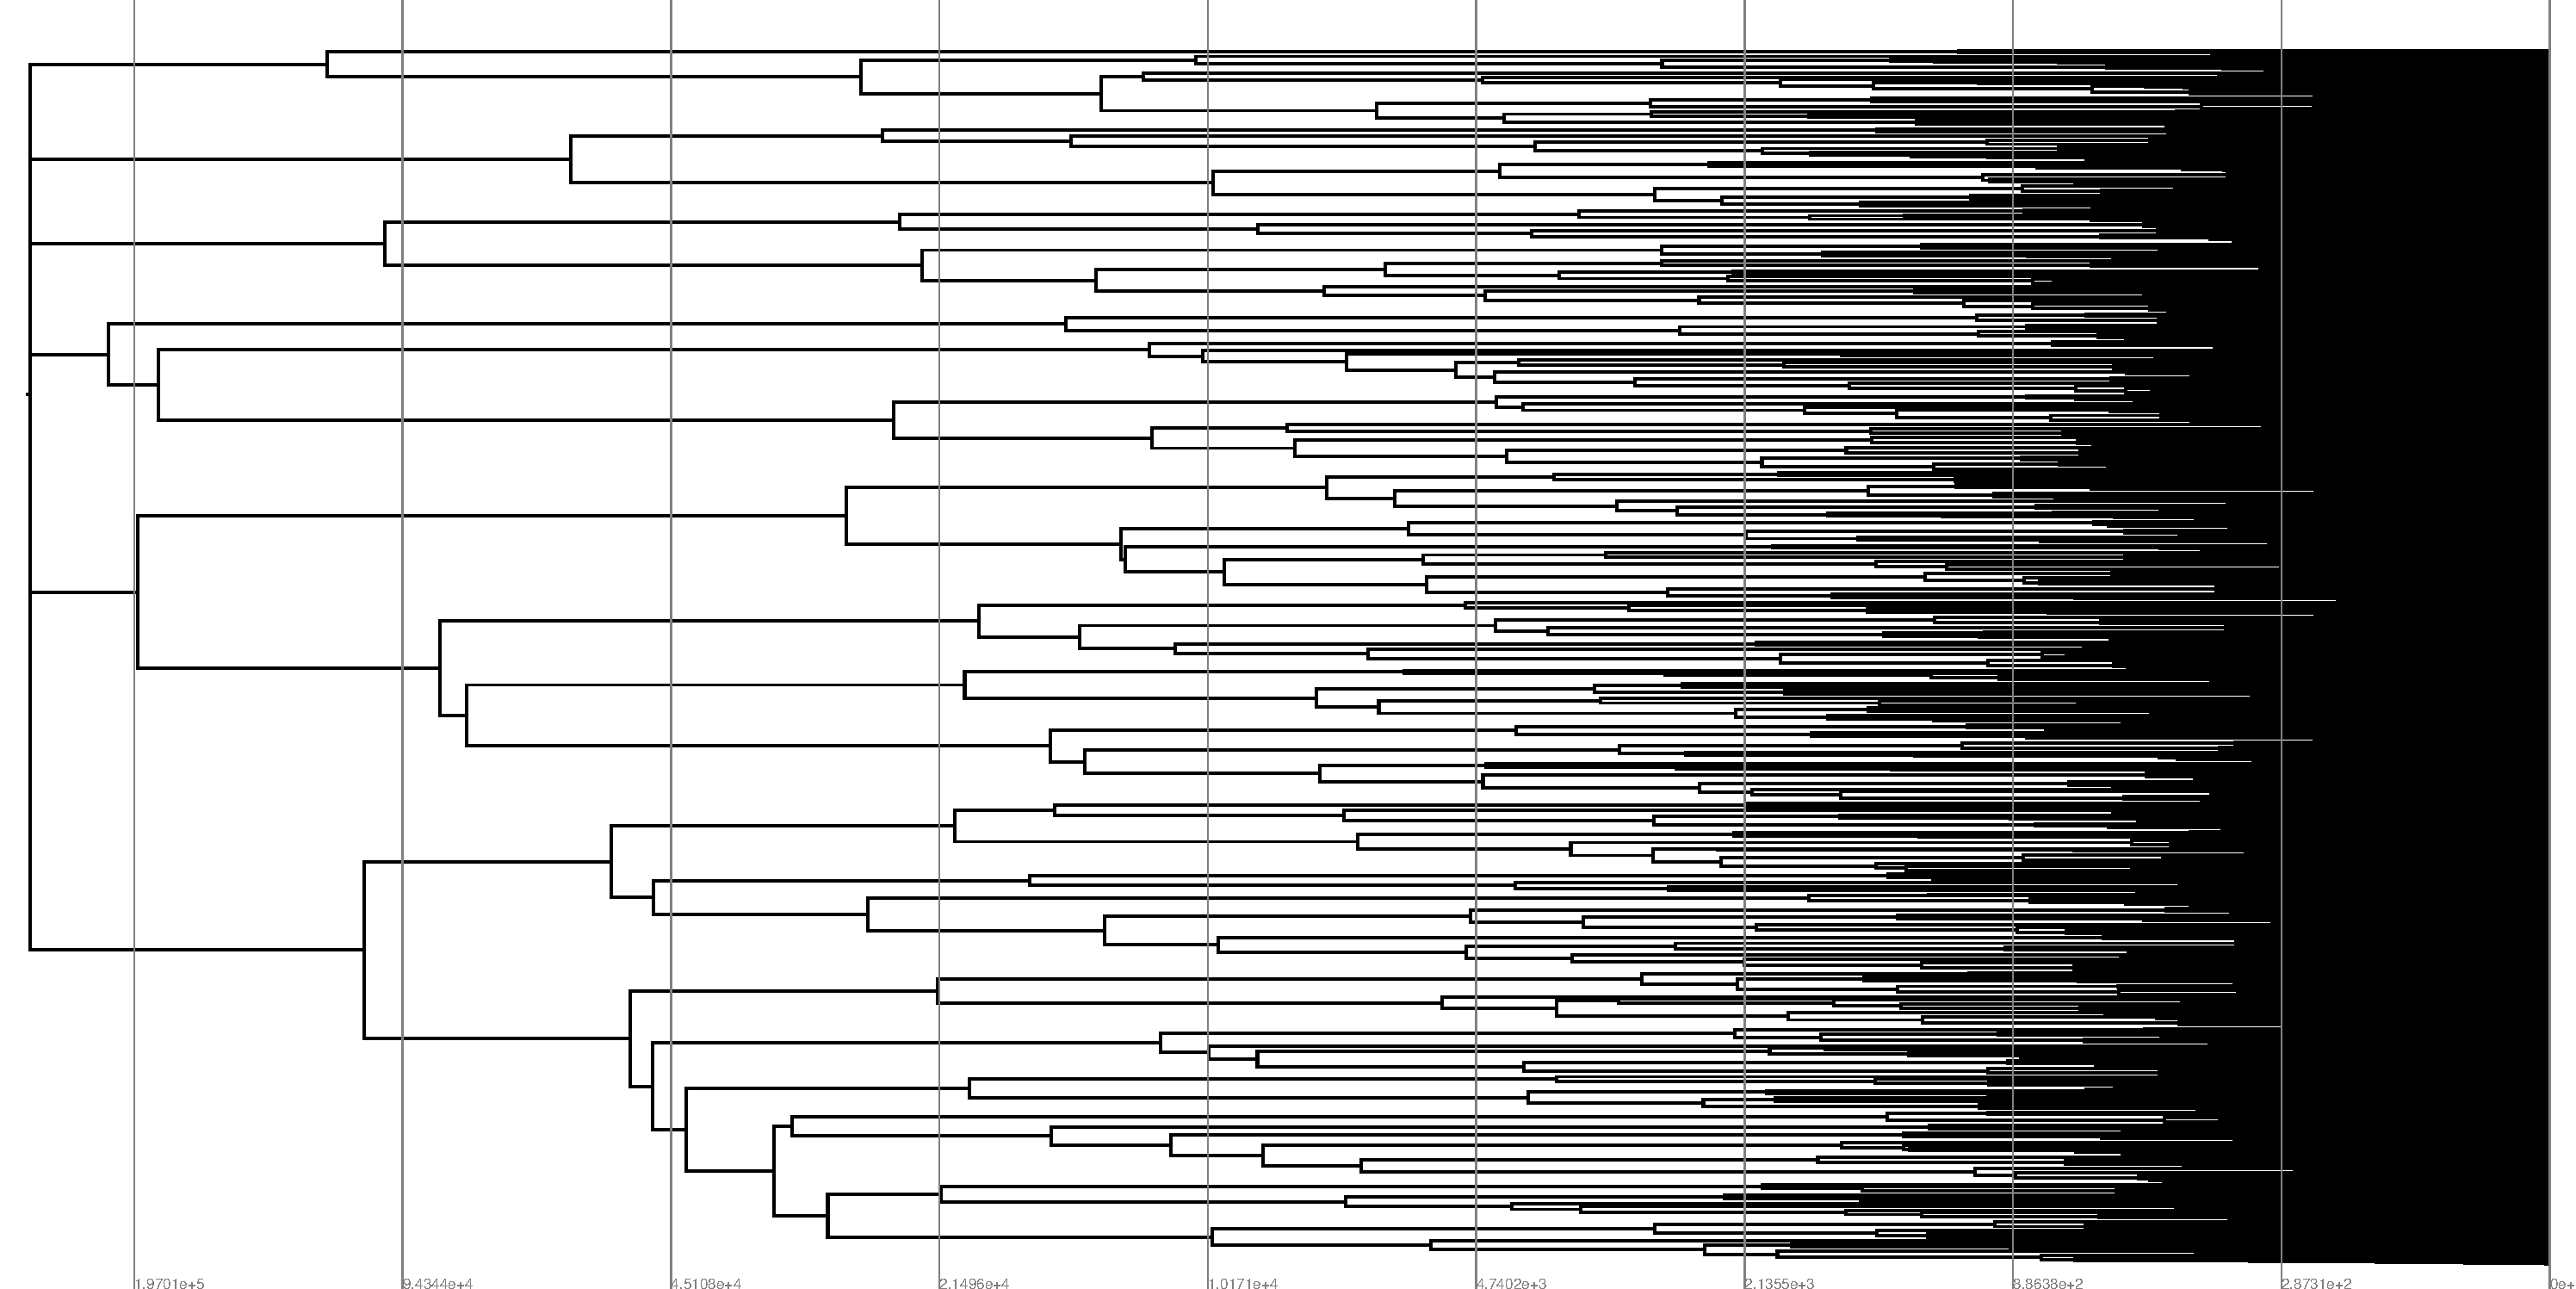
\includegraphics[height=0.12\textheight,width=\textwidth]{img/perfect-tree-phylogenies-log/epoch=7+resolution=3+treatment=22.pdf}
    % \end{noindent}
    \caption{%
      4 niche ecology with spatial structure}
    % \label{fig:perfect-tree-phylogenies-log:TODO}
  \end{subfigure}
  \hfill
  \begin{subfigure}[b]{0.5\columnwidth}
    % \begin{noindent}
    % 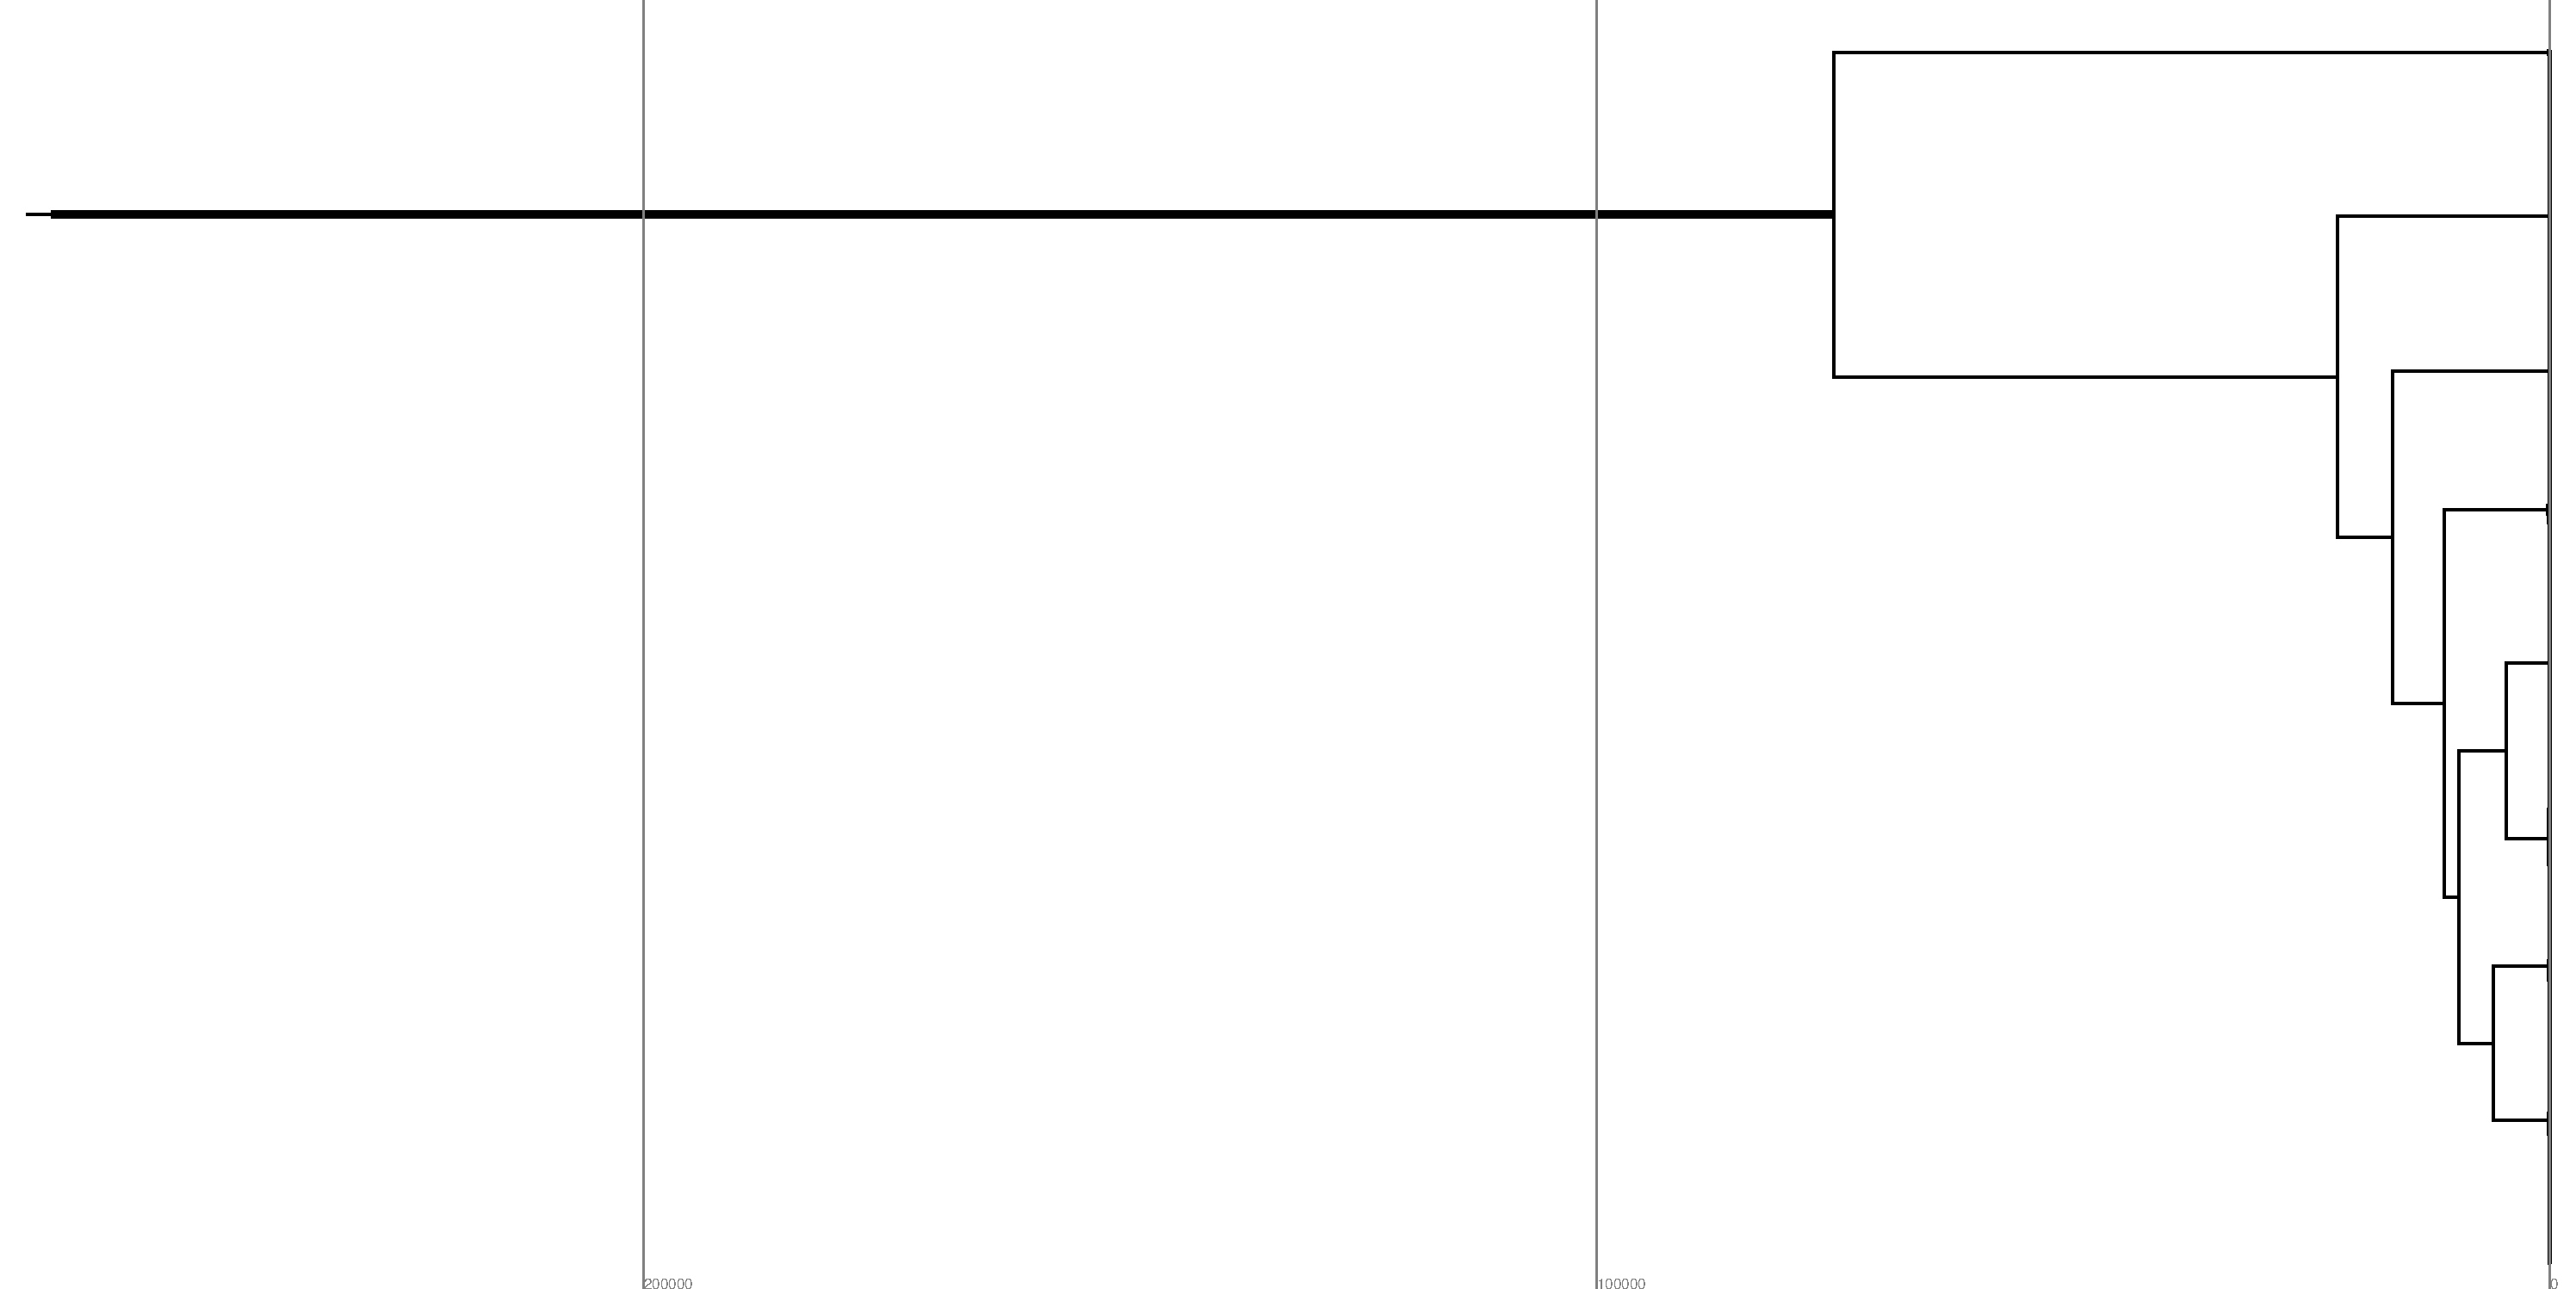
\includegraphics[height=0.12\textheight,width=\textwidth]{img/perfect-tree-phylogenies-log/epoch=7+resolution=3+treatment=20/a=collapsed-phylogeny+epoch=00007+mut_distn=np.random.standard_normal+num_generations=32768+num_islands=1+num_niches=8+p_island_migration=0.01+p_niche_invasion=3.0517578125e-08+population_size=32768+r.../eplicate=0+tournament_size=2+treatment=20+_generation=262144+_index=20+scale=nonlog+ext=.pdf}
    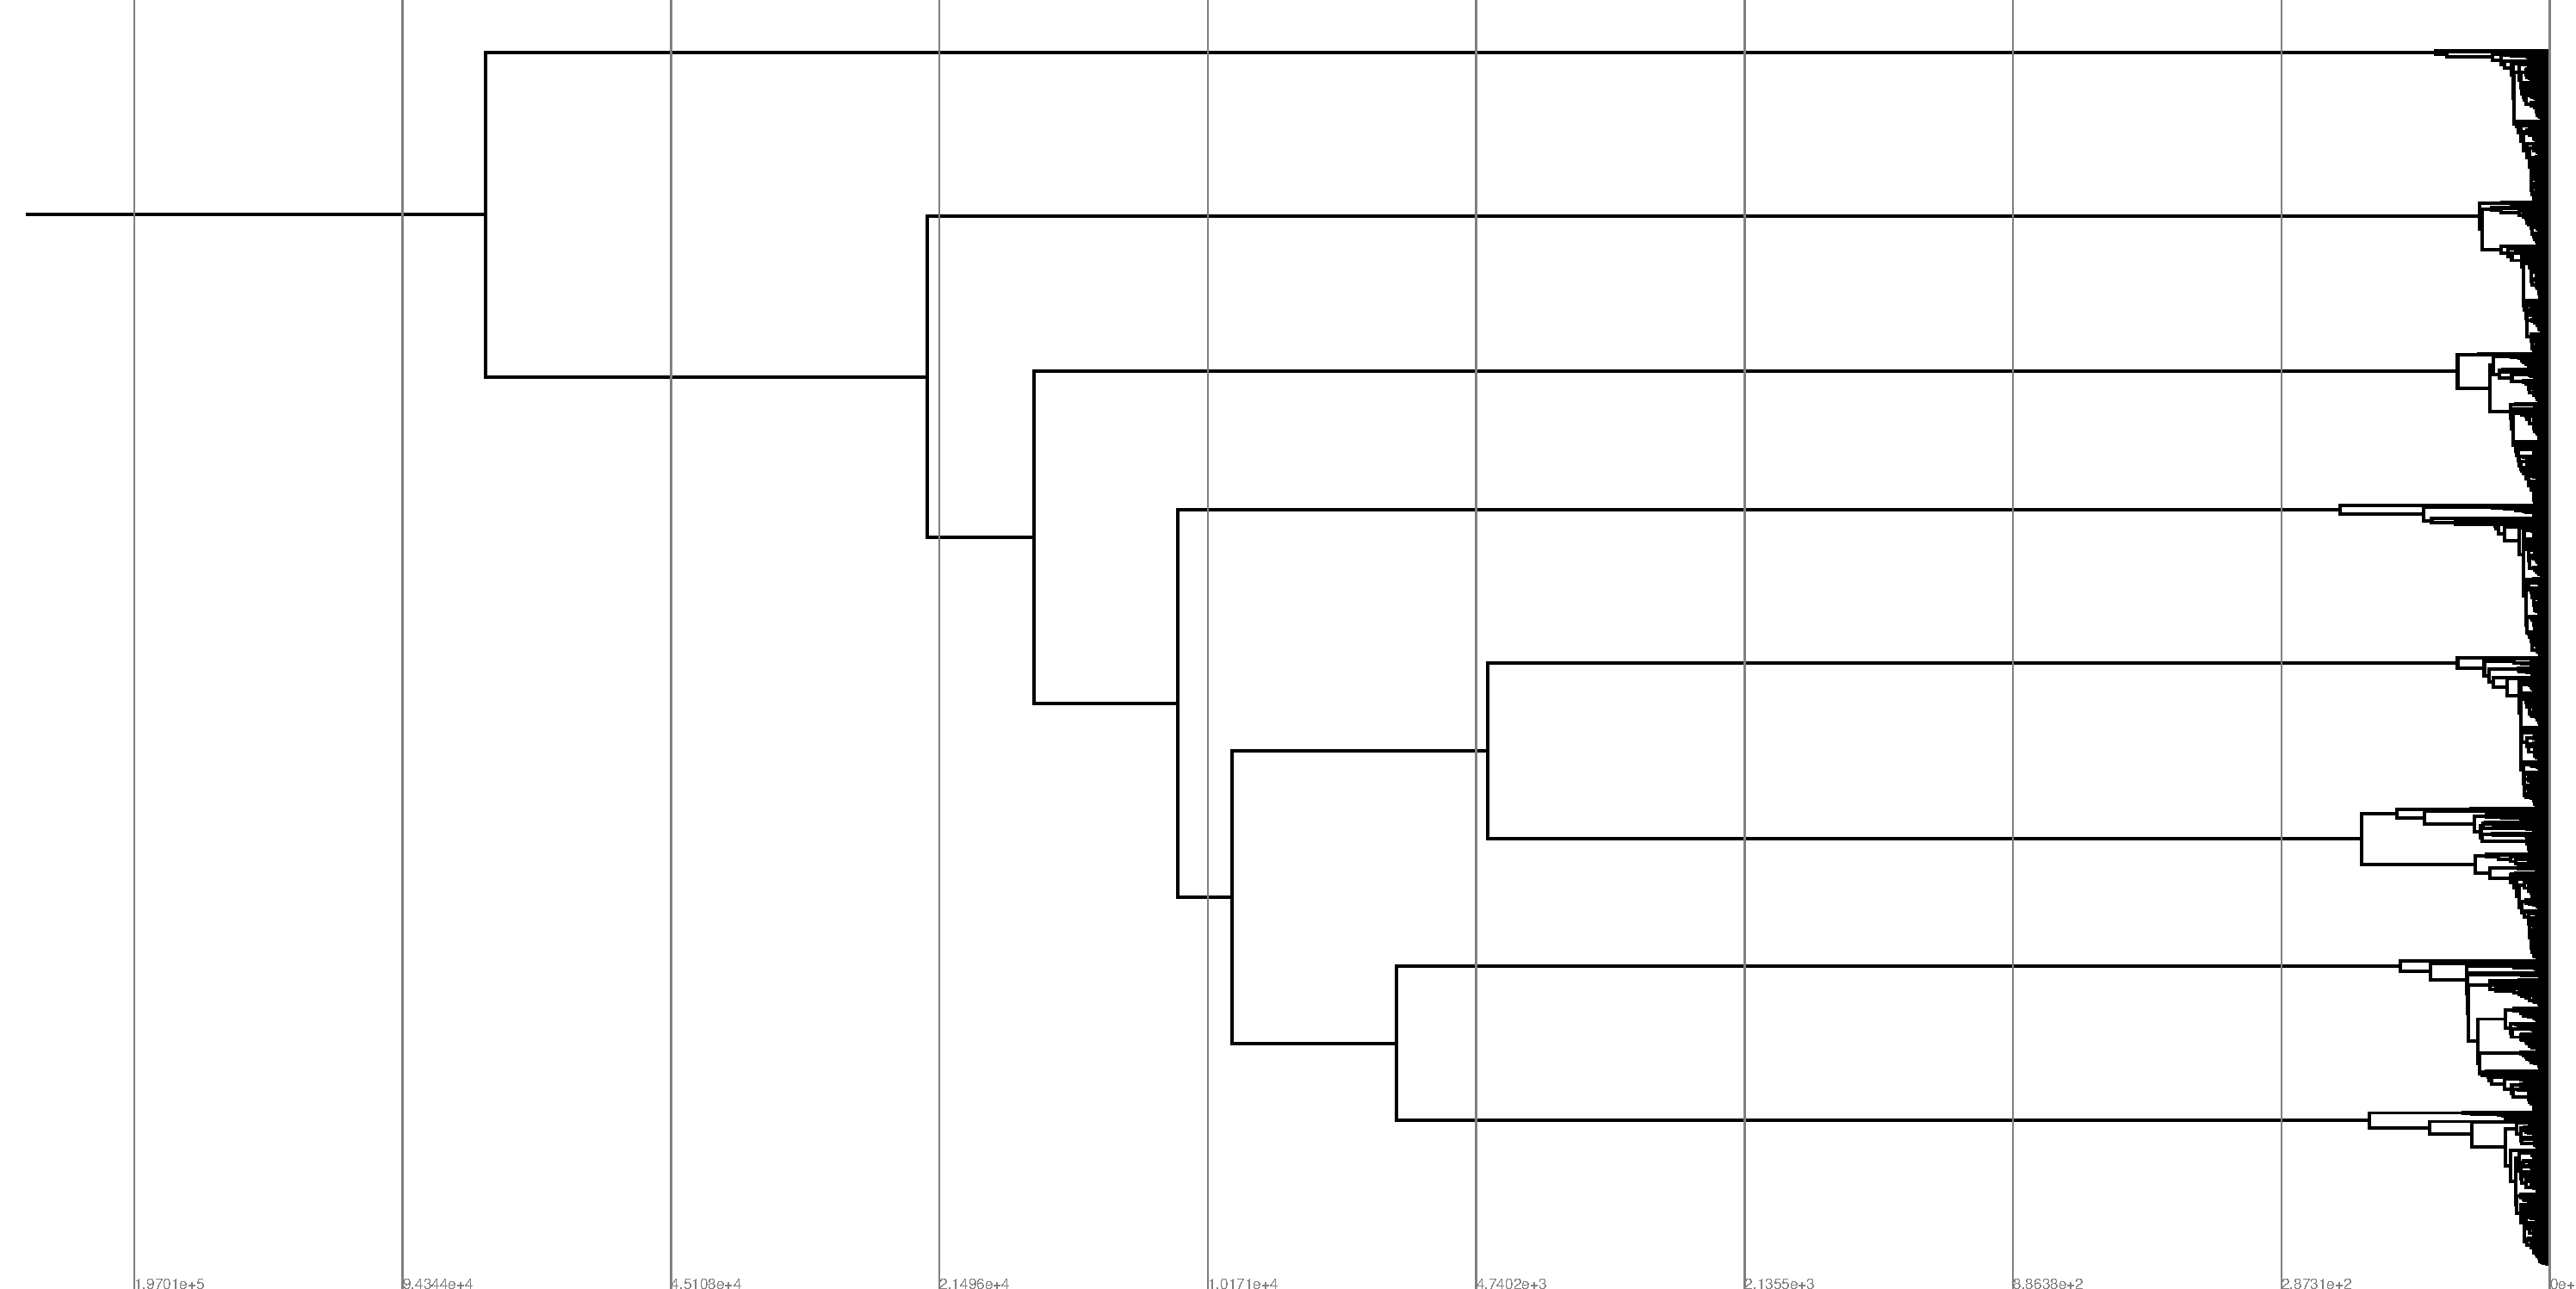
\includegraphics[height=0.12\textheight,width=\textwidth]{img/perfect-tree-phylogenies-log/epoch=7+resolution=3+treatment=20.pdf}
    % \end{noindent}
    \caption{%
      8 niche ecology}
    % \label{fig:perfect-tree-phylogenies-log:TODO}
  \end{subfigure}
  \hfill
  \begin{subfigure}[b]{0.5\columnwidth}
    % \begin{noindent}
    % 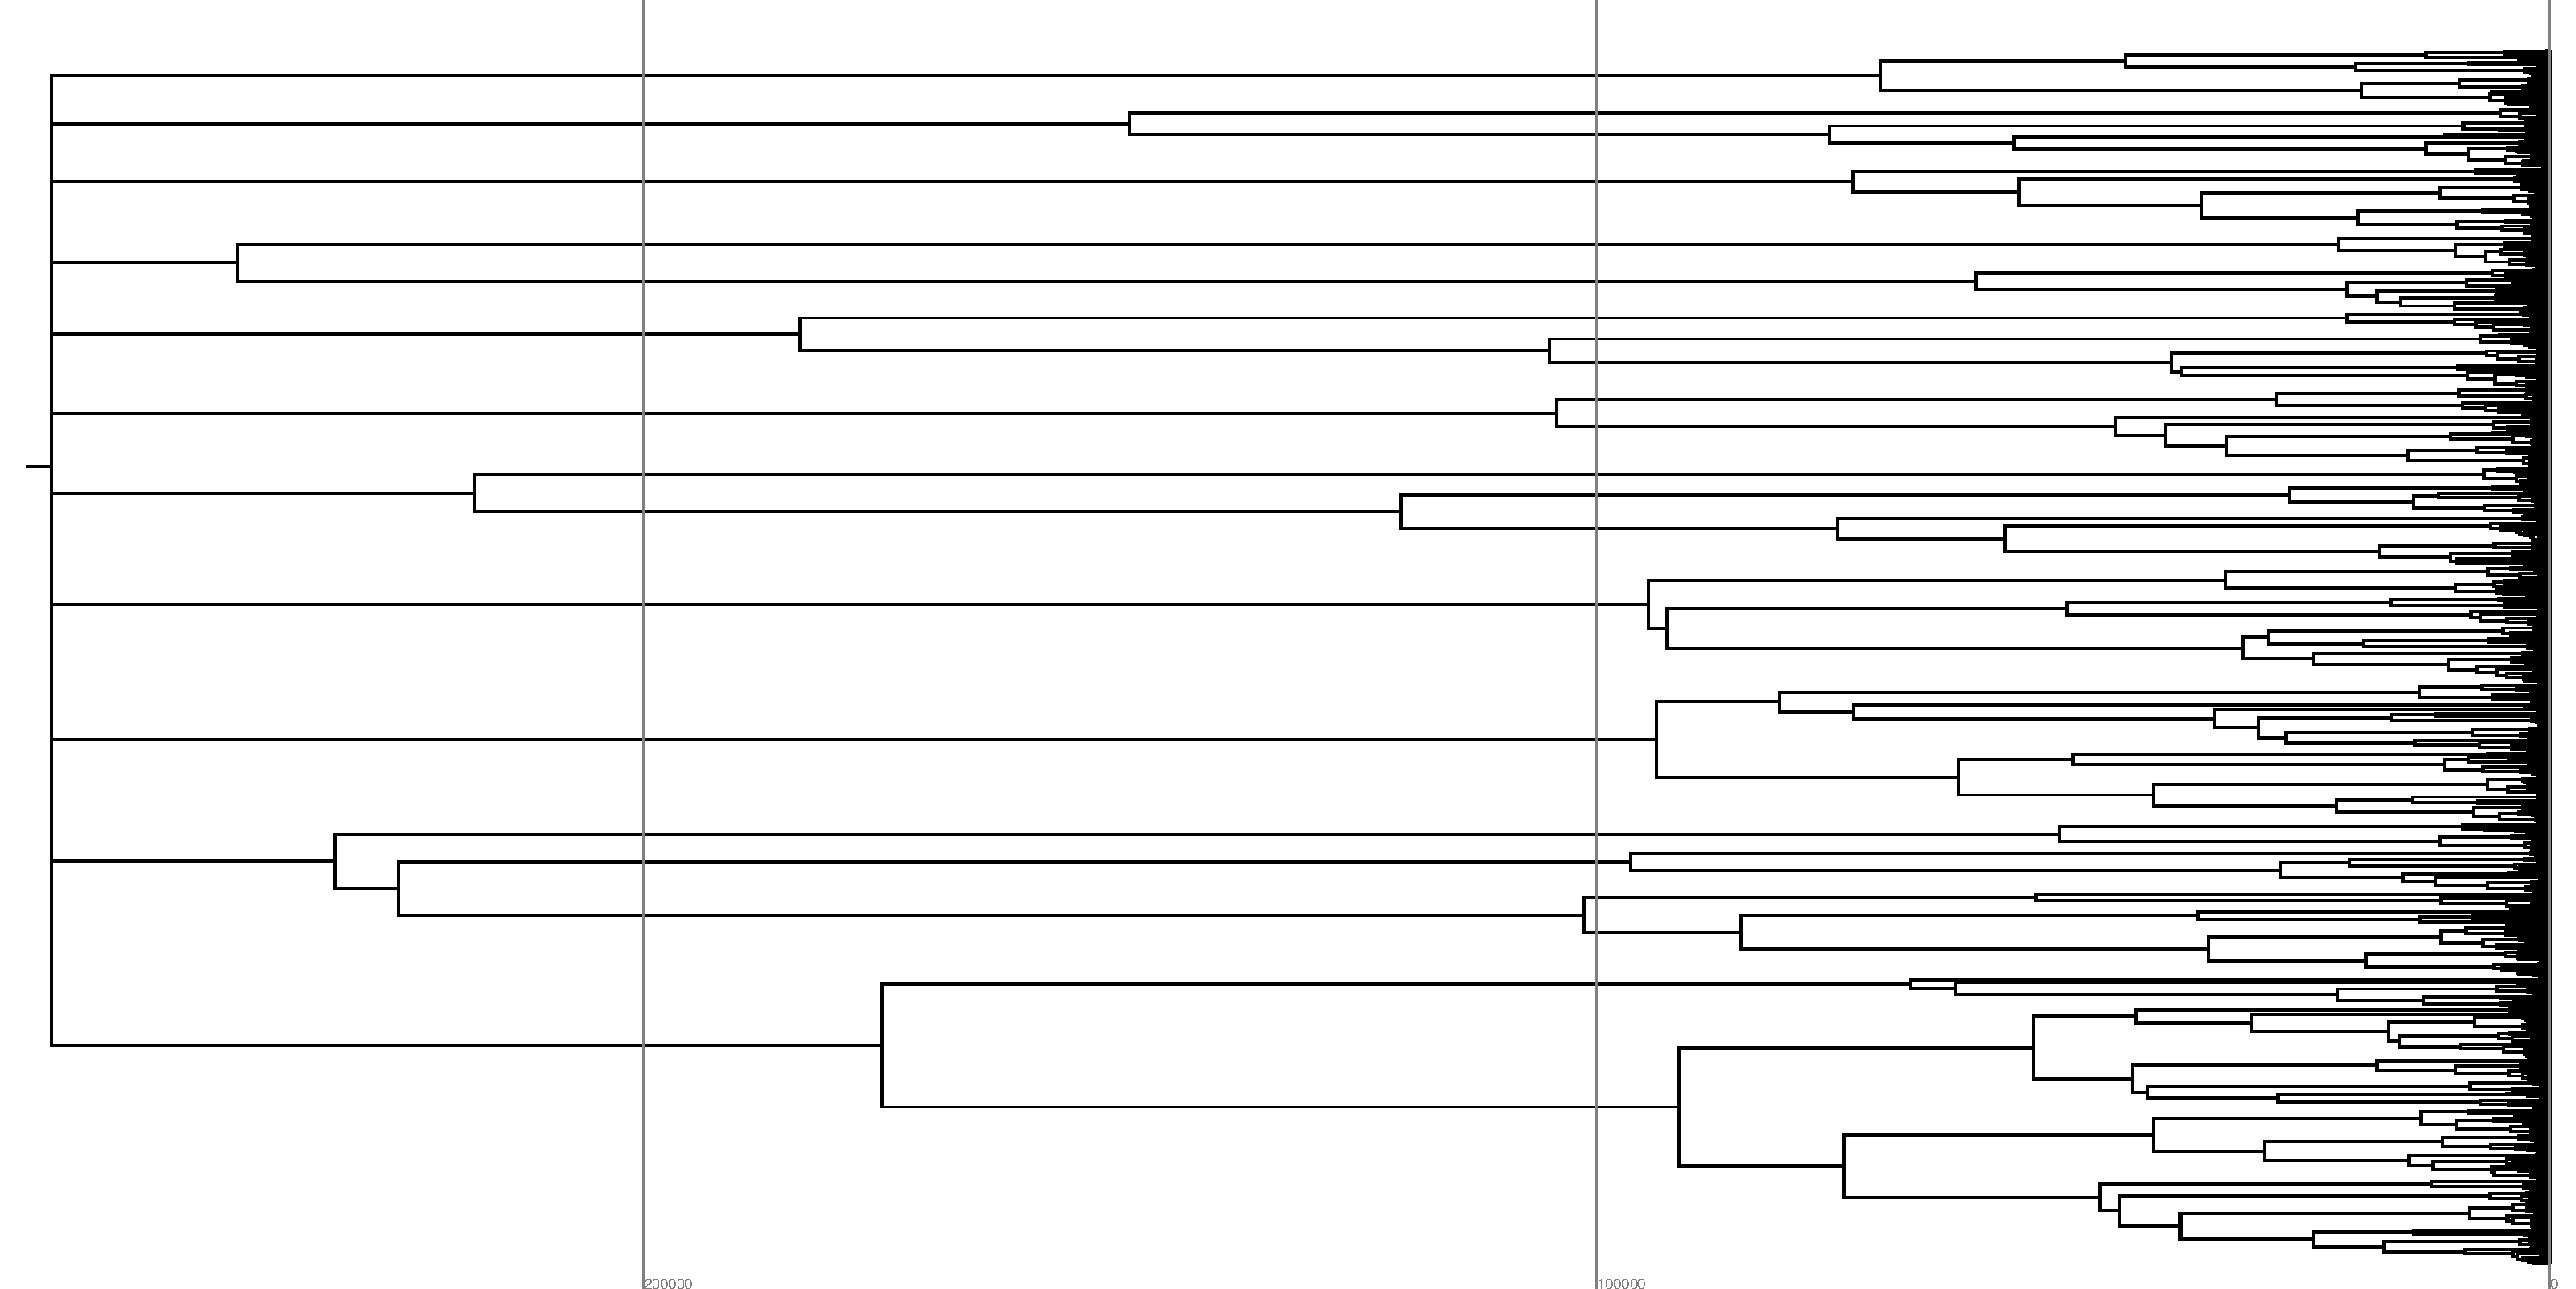
\includegraphics[height=0.12\textheight,width=\textwidth]{img/perfect-tree-phylogenies-log/epoch=7+resolution=3+treatment=18/a=collapsed-phylogeny+epoch=00007+mut_distn=np.random.standard_normal+num_generations=32768+num_islands=1024+num_niches=8+p_island_migration=0.01+p_niche_invasion=3.0517578125e-08+population_size=3276.../8+replicate=0+tournament_size=2+treatment=18+_generation=262144+_index=18+scale=nonlog+ext=.pdf}
    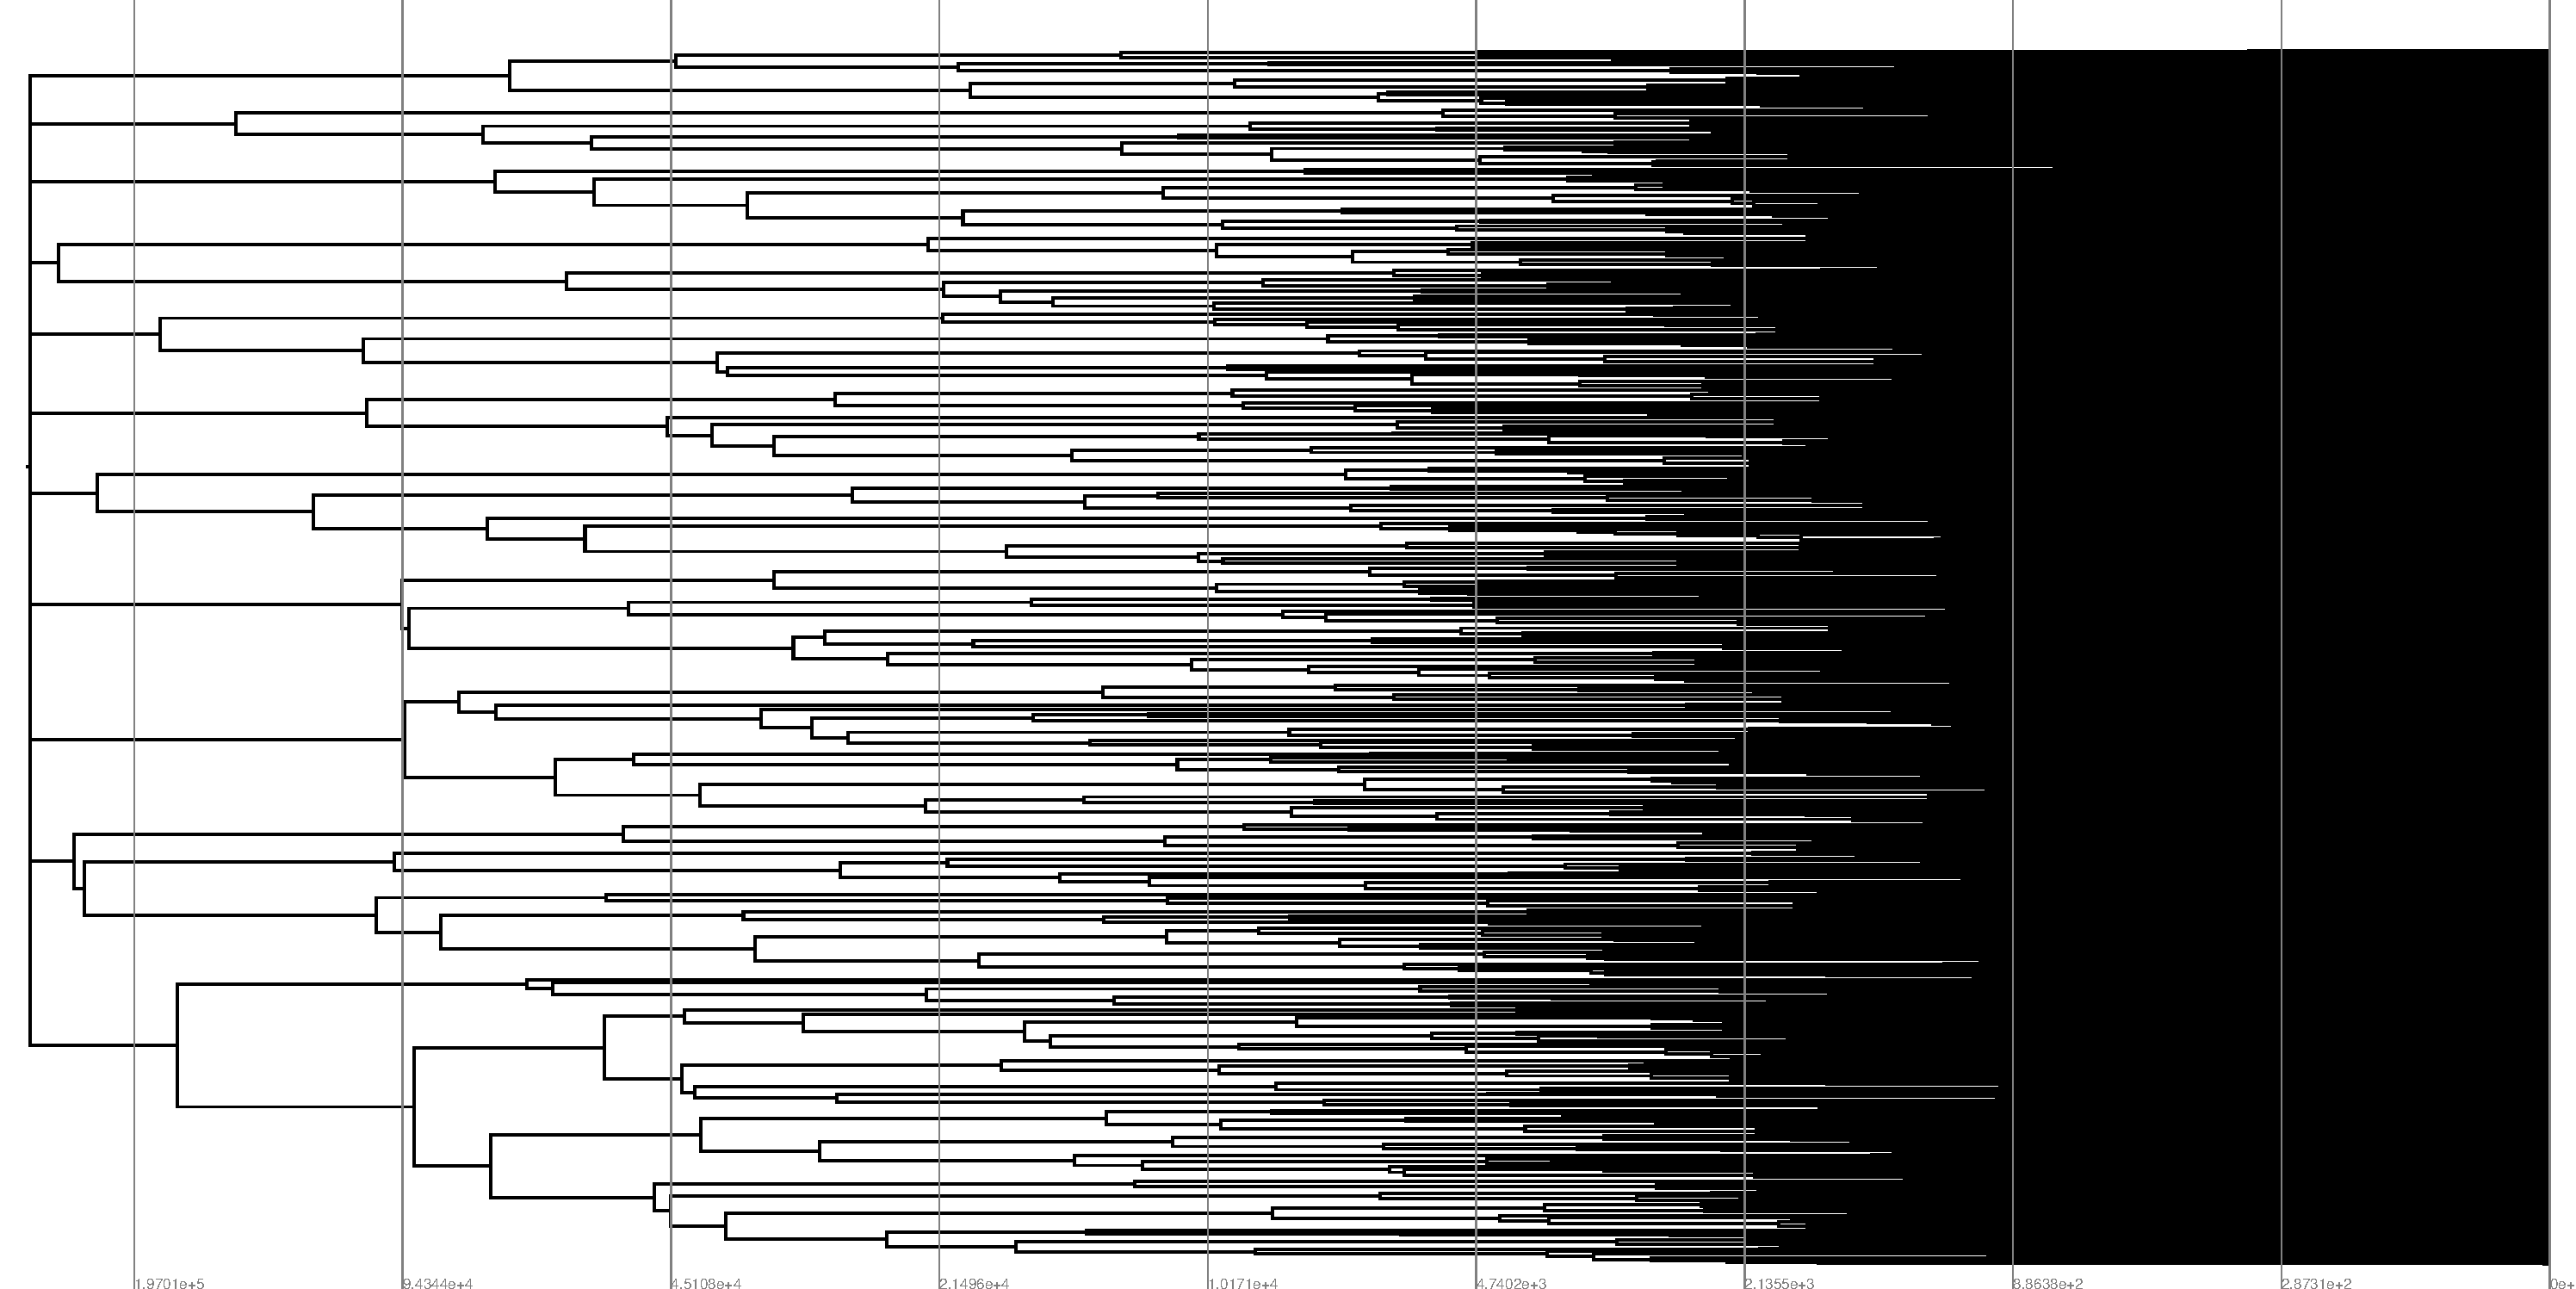
\includegraphics[height=0.12\textheight,width=\textwidth]{img/perfect-tree-phylogenies-log/epoch=7+resolution=3+treatment=18.pdf}
    % \end{noindent}
    \caption{%
      8 niche ecology with spatial structure}
    % \label{fig:perfect-tree-phylogenies-log:TODO}
  \end{subfigure}
  \hfill
  \caption{%
    \textbf{Sample reference phylogenies from the simple model across evolutionary regimes.}
    Each phylogeny has 32,768 leaves.
    Note linear-scale $x$ axis.
  }
  \label{fig:perfect-tree-phylogenies-nonlog}
\end{figure*}

% \begin{subfigure}[b]{0.5\columnwidth}
% % \begin{noindent}
% 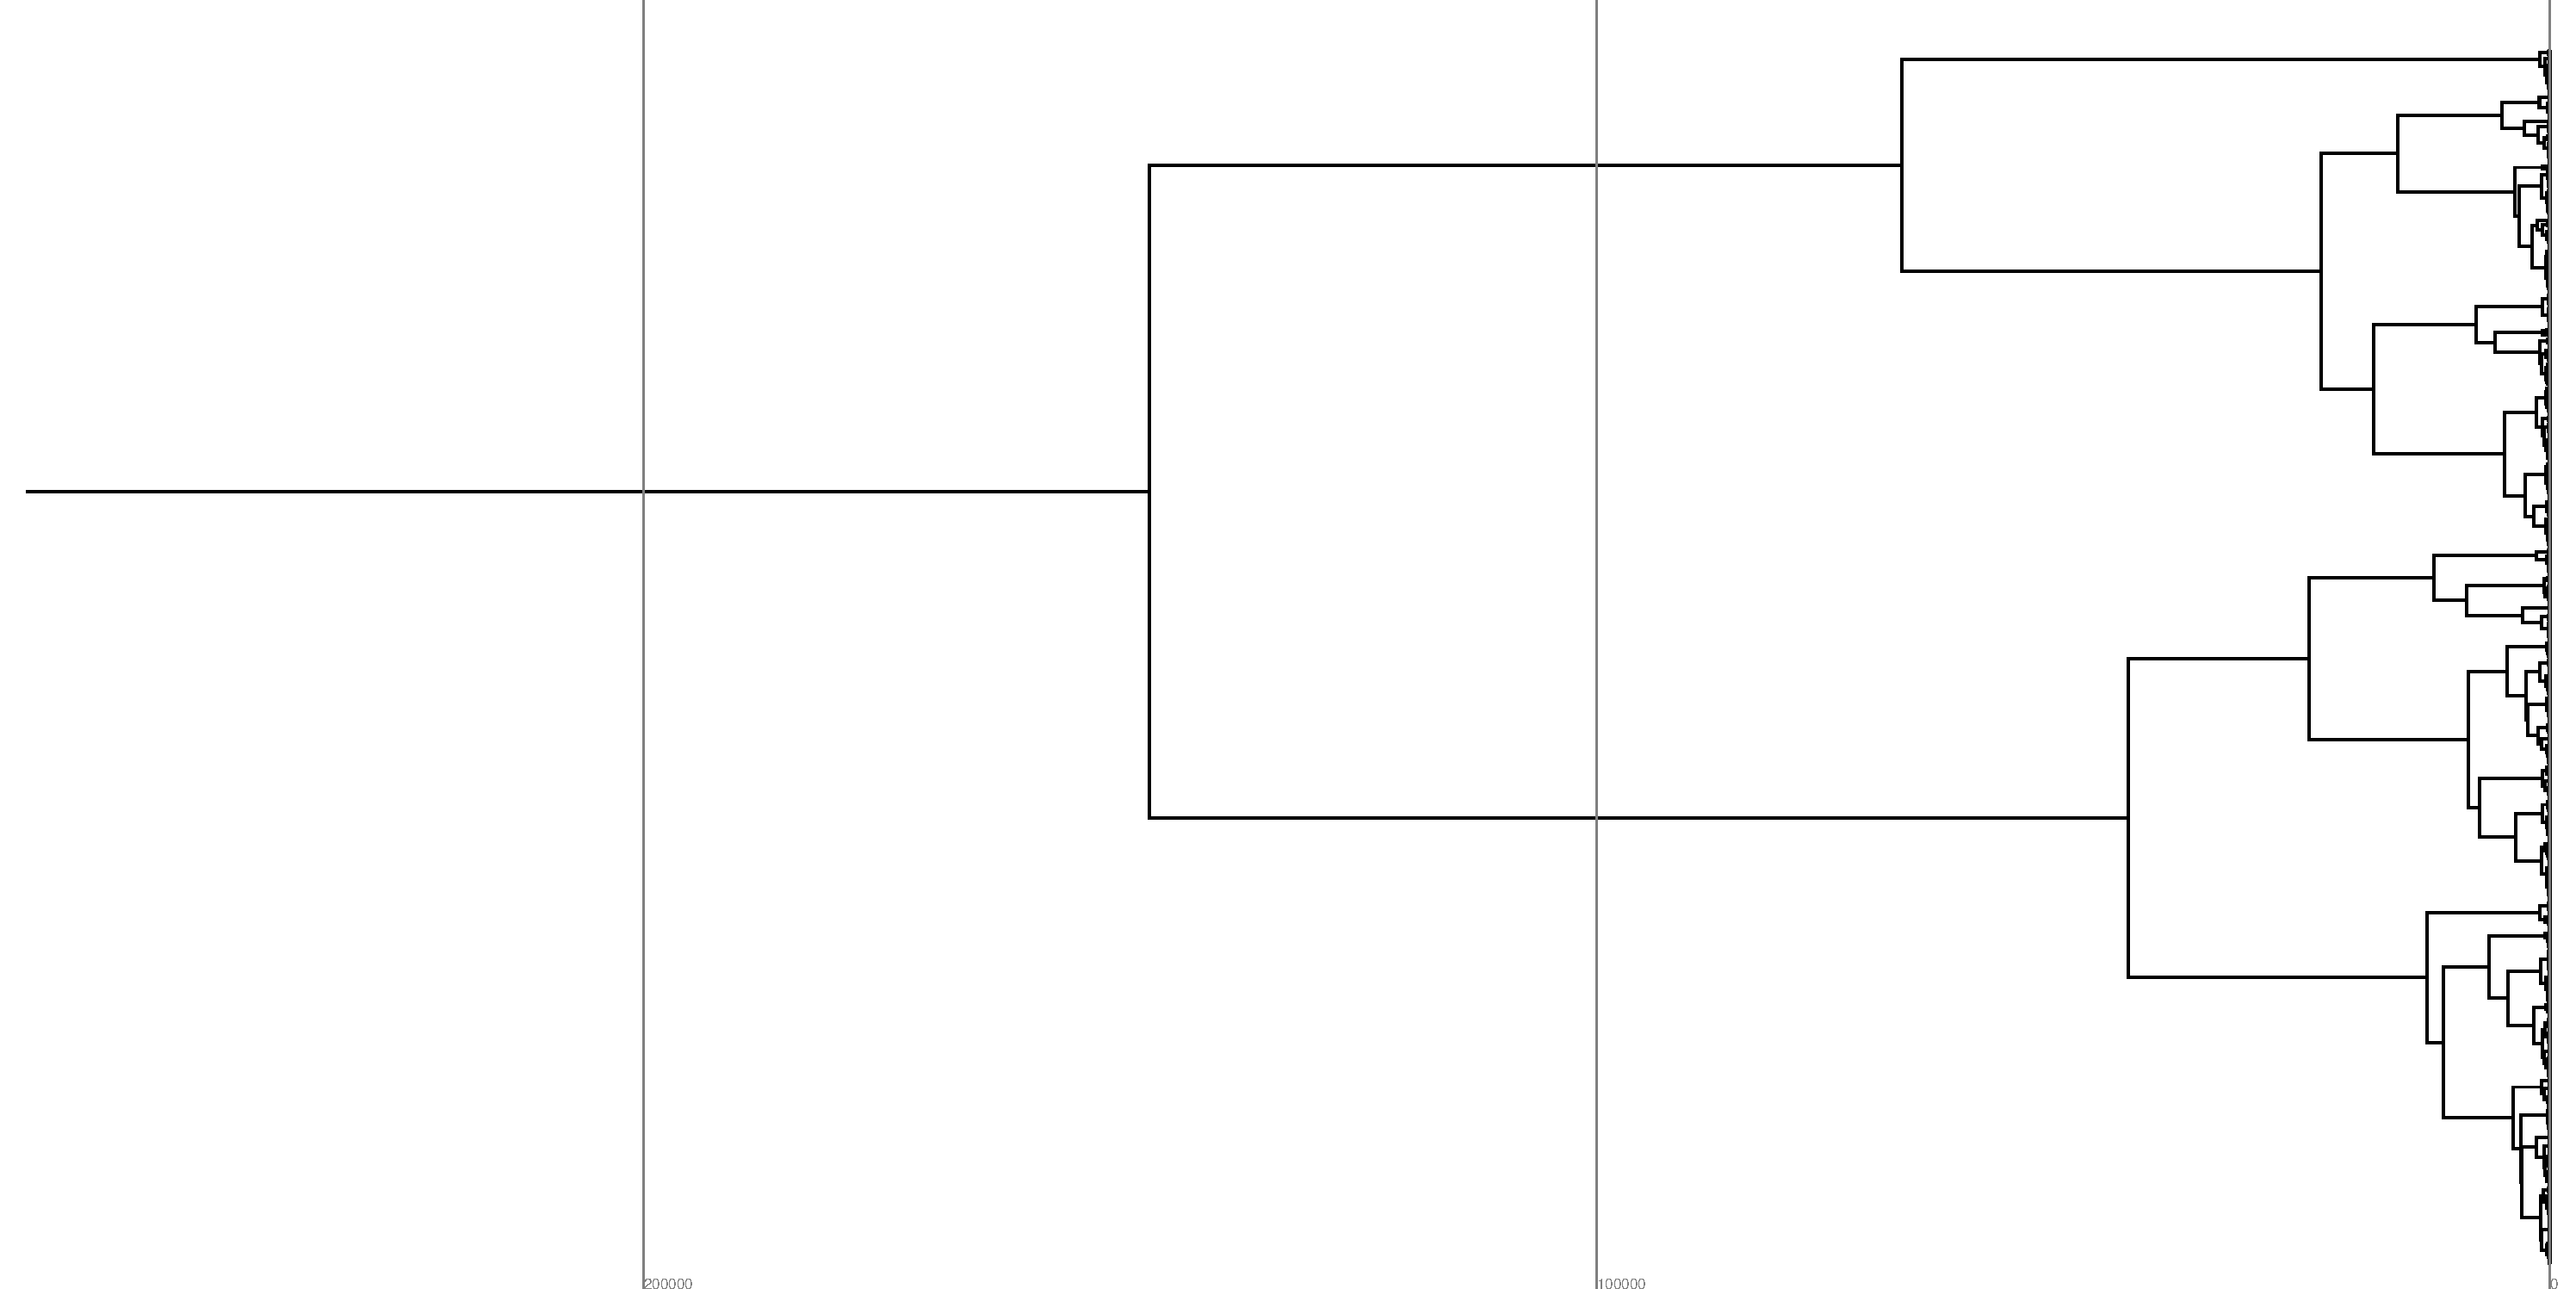
\includegraphics[height=0.12\textheight,width=\textwidth]{img/perfect-tree-phylogenies-log/epoch=7+resolution=3+treatment=0/a=collapsed-phylogeny+epoch=00007+mut_distn=np.random.standard_normal+num_generations=32768+num_islands=1024+num_niches=1+p_island_migration=0.01+p_niche_invasion=3.0517578125e-08+population_size=3276.../8+replicate=0+tournament_size=4+treatment=0+_generation=262144+_index=0+scale=nonlog+ext=.pdf}
% % \end{noindent}
% \caption{%
% spatial structure strong election}
% % \label{fig:perfect-tree-phylogenies-log:TODO}
% \end{subfigure}

% \begin{subfigure}[b]{0.5\columnwidth}
% % \begin{noindent}
% 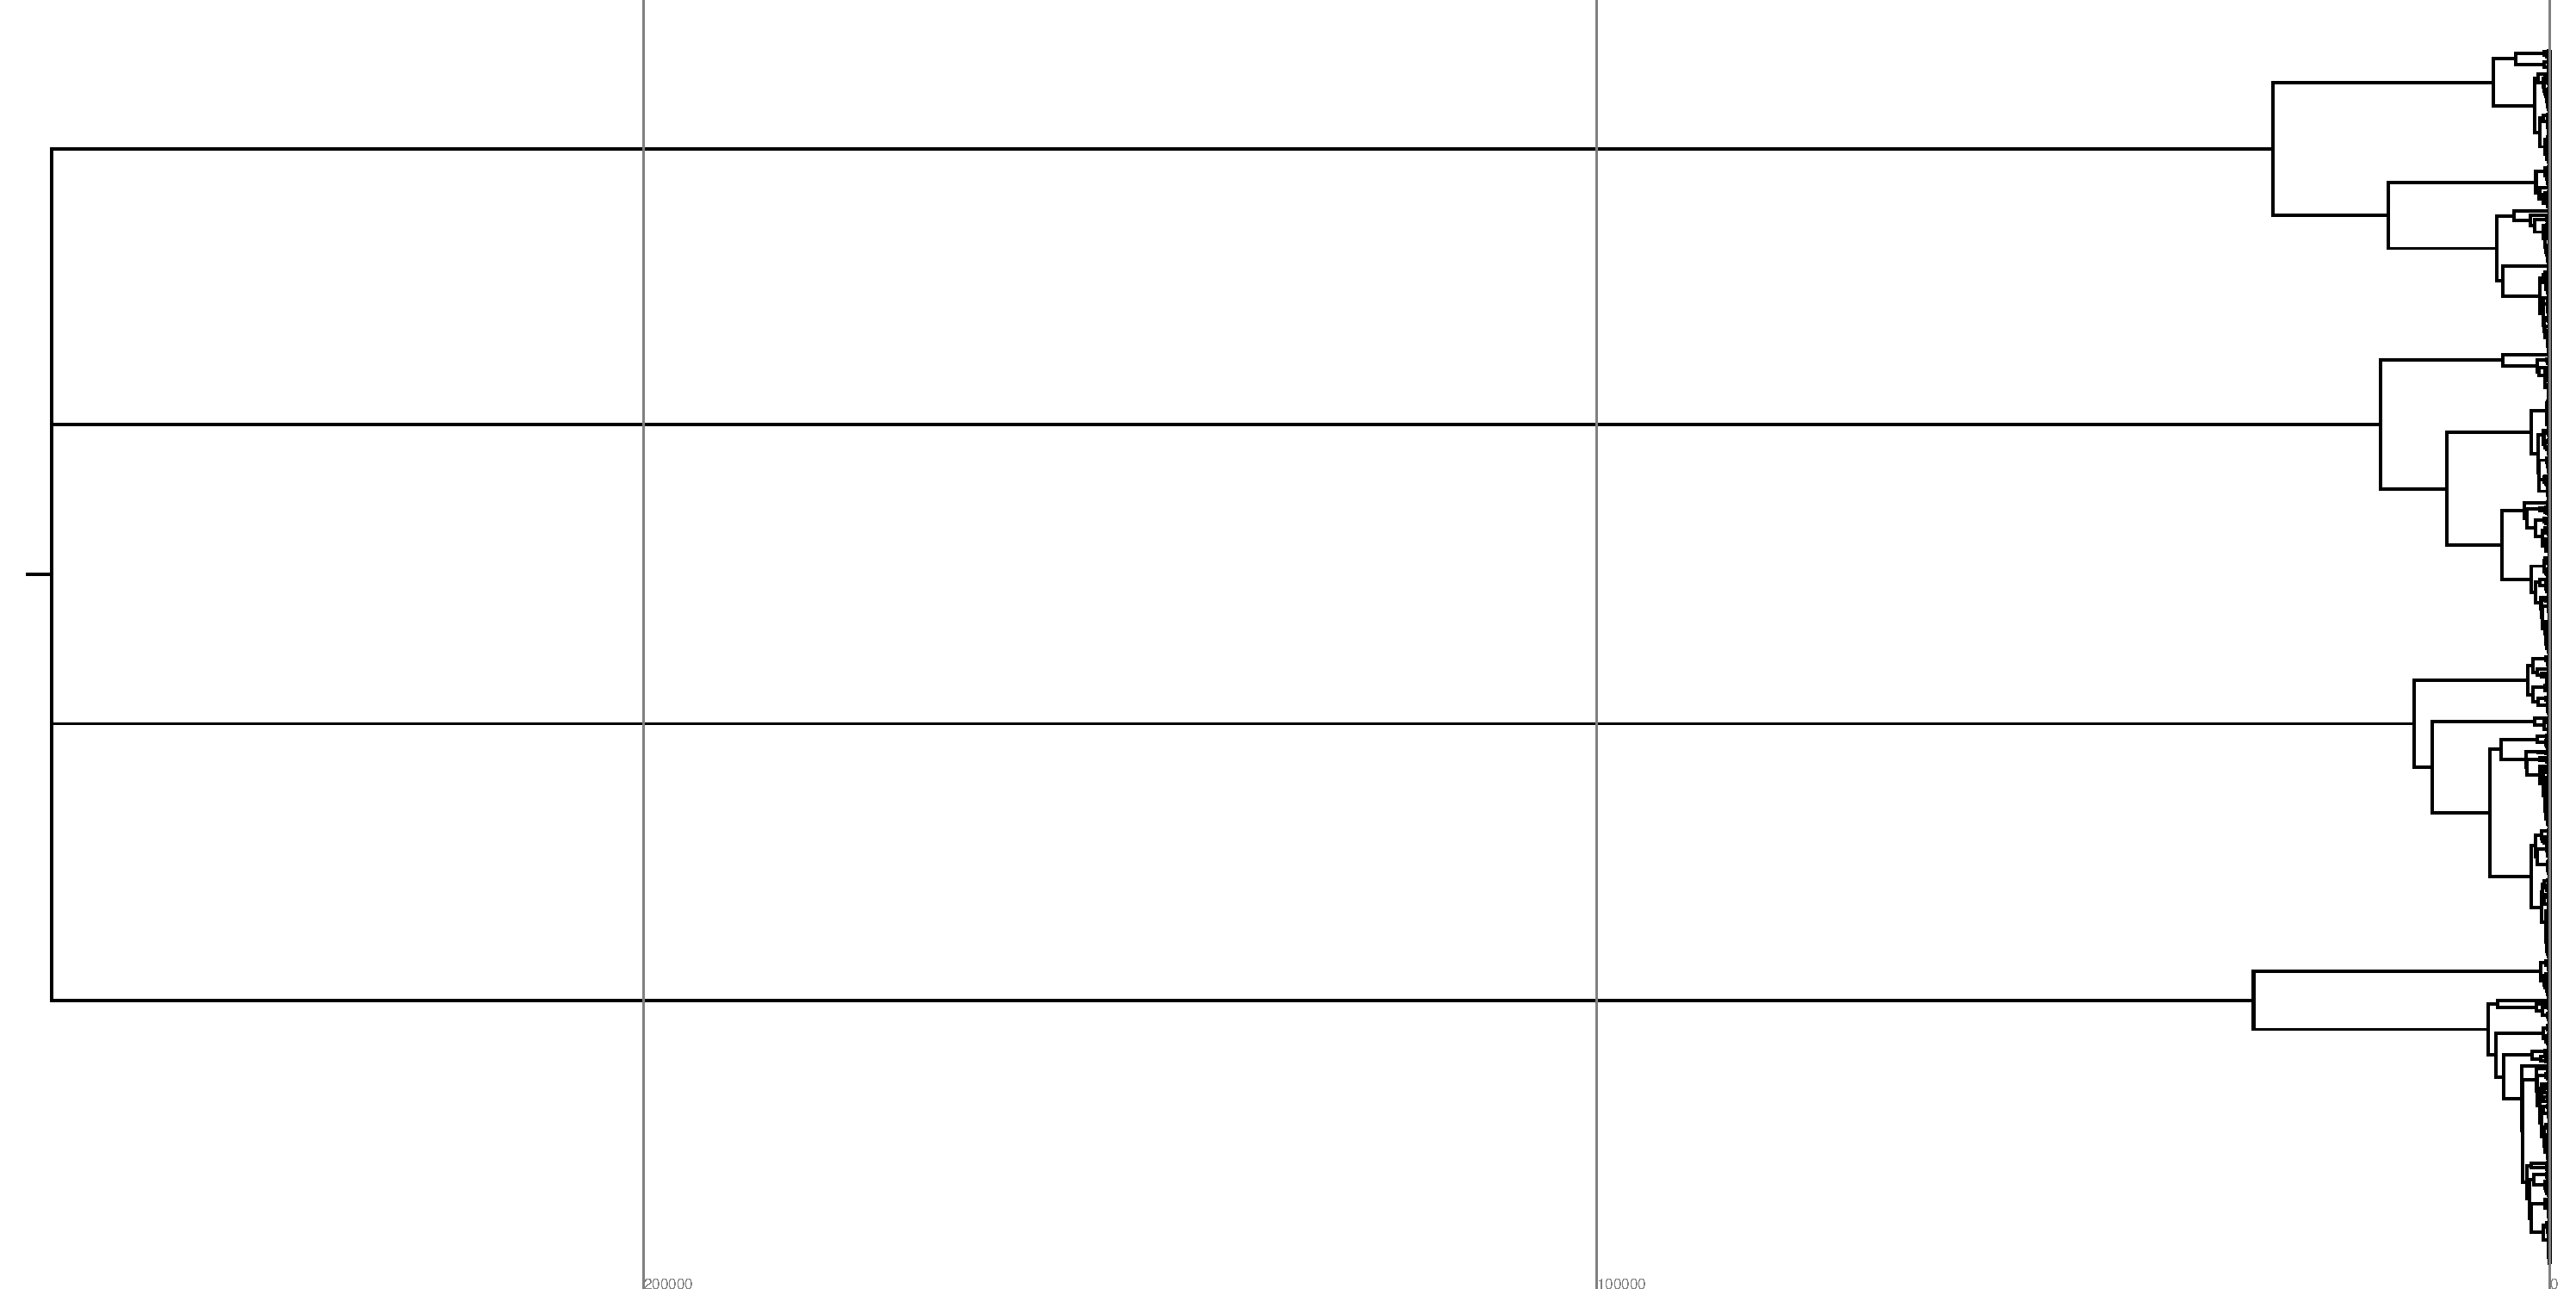
\includegraphics[height=0.12\textheight,width=\textwidth]{img/perfect-tree-phylogenies-log/epoch=7+resolution=3+treatment=16/a=collapsed-phylogeny+epoch=00007+mut_distn=np.random.standard_normal+num_generations=32768+num_islands=1+num_niches=4+p_island_migration=0.01+p_niche_invasion=3.0517578125e-08+population_size=32768+r.../eplicate=0+tournament_size=1+treatment=16+_generation=262144+_index=16+scale=nonlog+ext=.pdf}
% % \end{noindent}
% \caption{%
% weak selection 4 niche ecology}
% % \label{fig:perfect-tree-phylogenies-log:TODO}
% \end{subfigure}

% \begin{subfigure}[b]{0.5\columnwidth}
% % \begin{noindent}
% 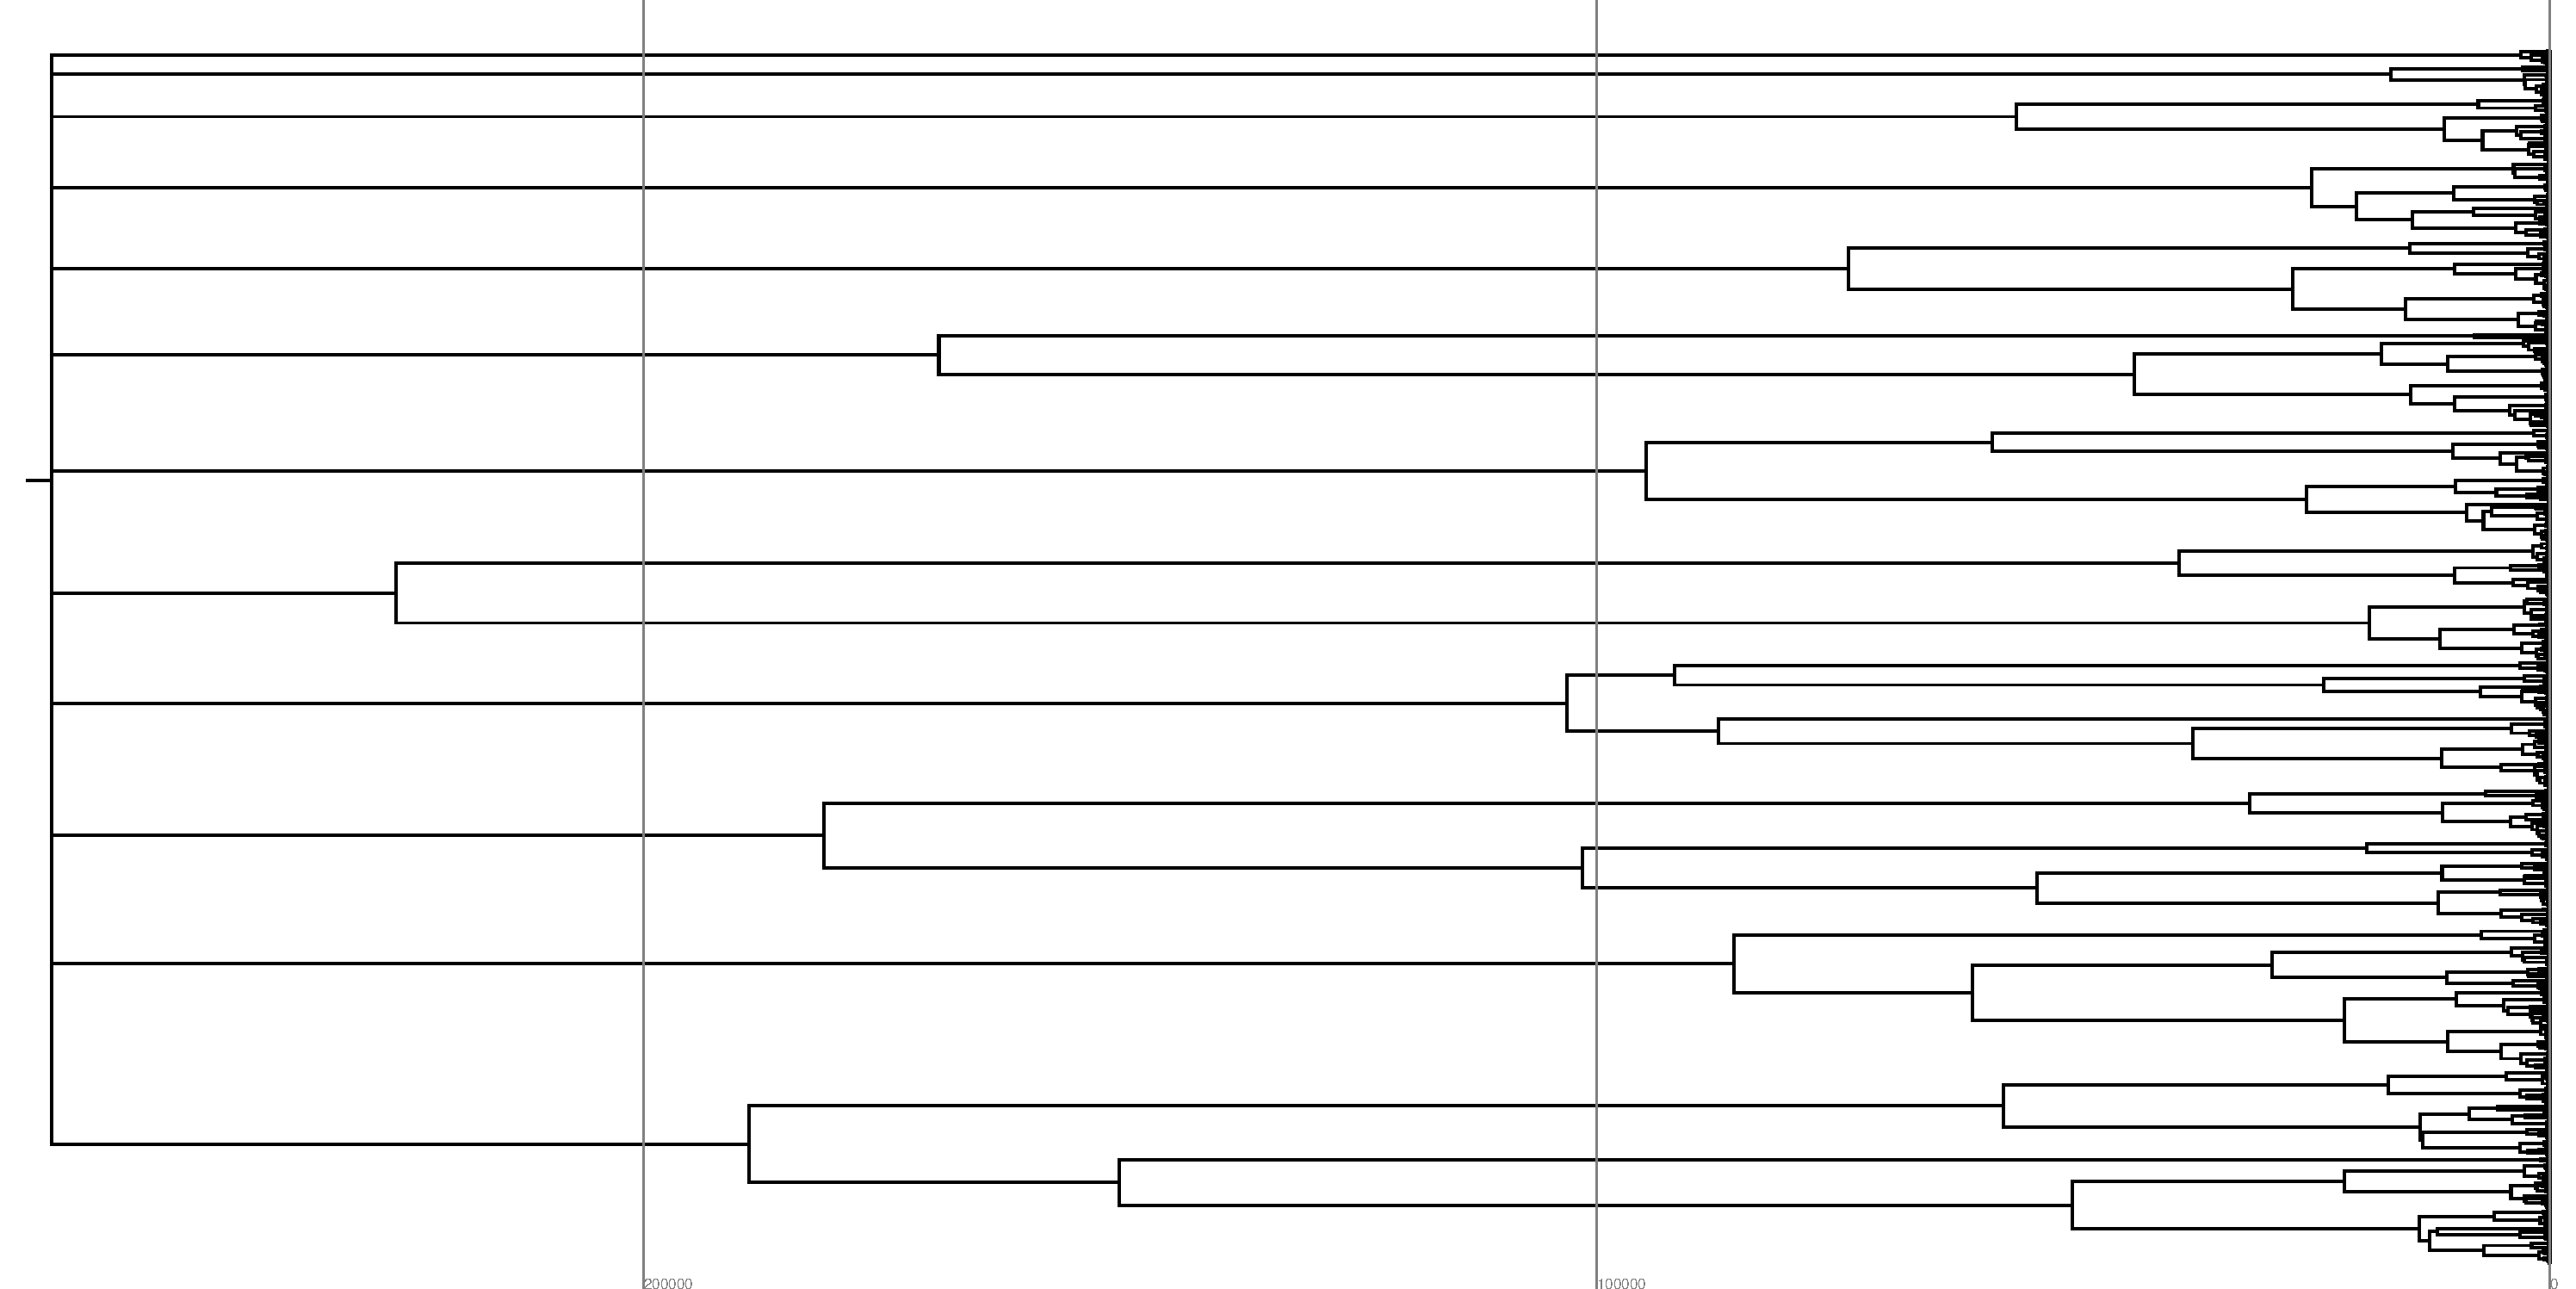
\includegraphics[height=0.12\textheight,width=\textwidth]{img/perfect-tree-phylogenies-log/epoch=7+resolution=3+treatment=12/a=collapsed-phylogeny+epoch=00007+mut_distn=np.random.standard_normal+num_generations=32768+num_islands=1024+num_niches=1+p_island_migration=0.01+p_niche_invasion=3.0517578125e-08+population_size=3276.../8+replicate=0+tournament_size=1+treatment=12+_generation=262144+_index=12+scale=nonlog+ext=.pdf}
% % \end{noindent}
% \caption{%
% spatial structure weak selection}
% % \label{fig:perfect-tree-phylogenies-log:TODO}
% \end{subfigure}

% \begin{subfigure}[b]{0.5\columnwidth}
% % \begin{noindent}
% 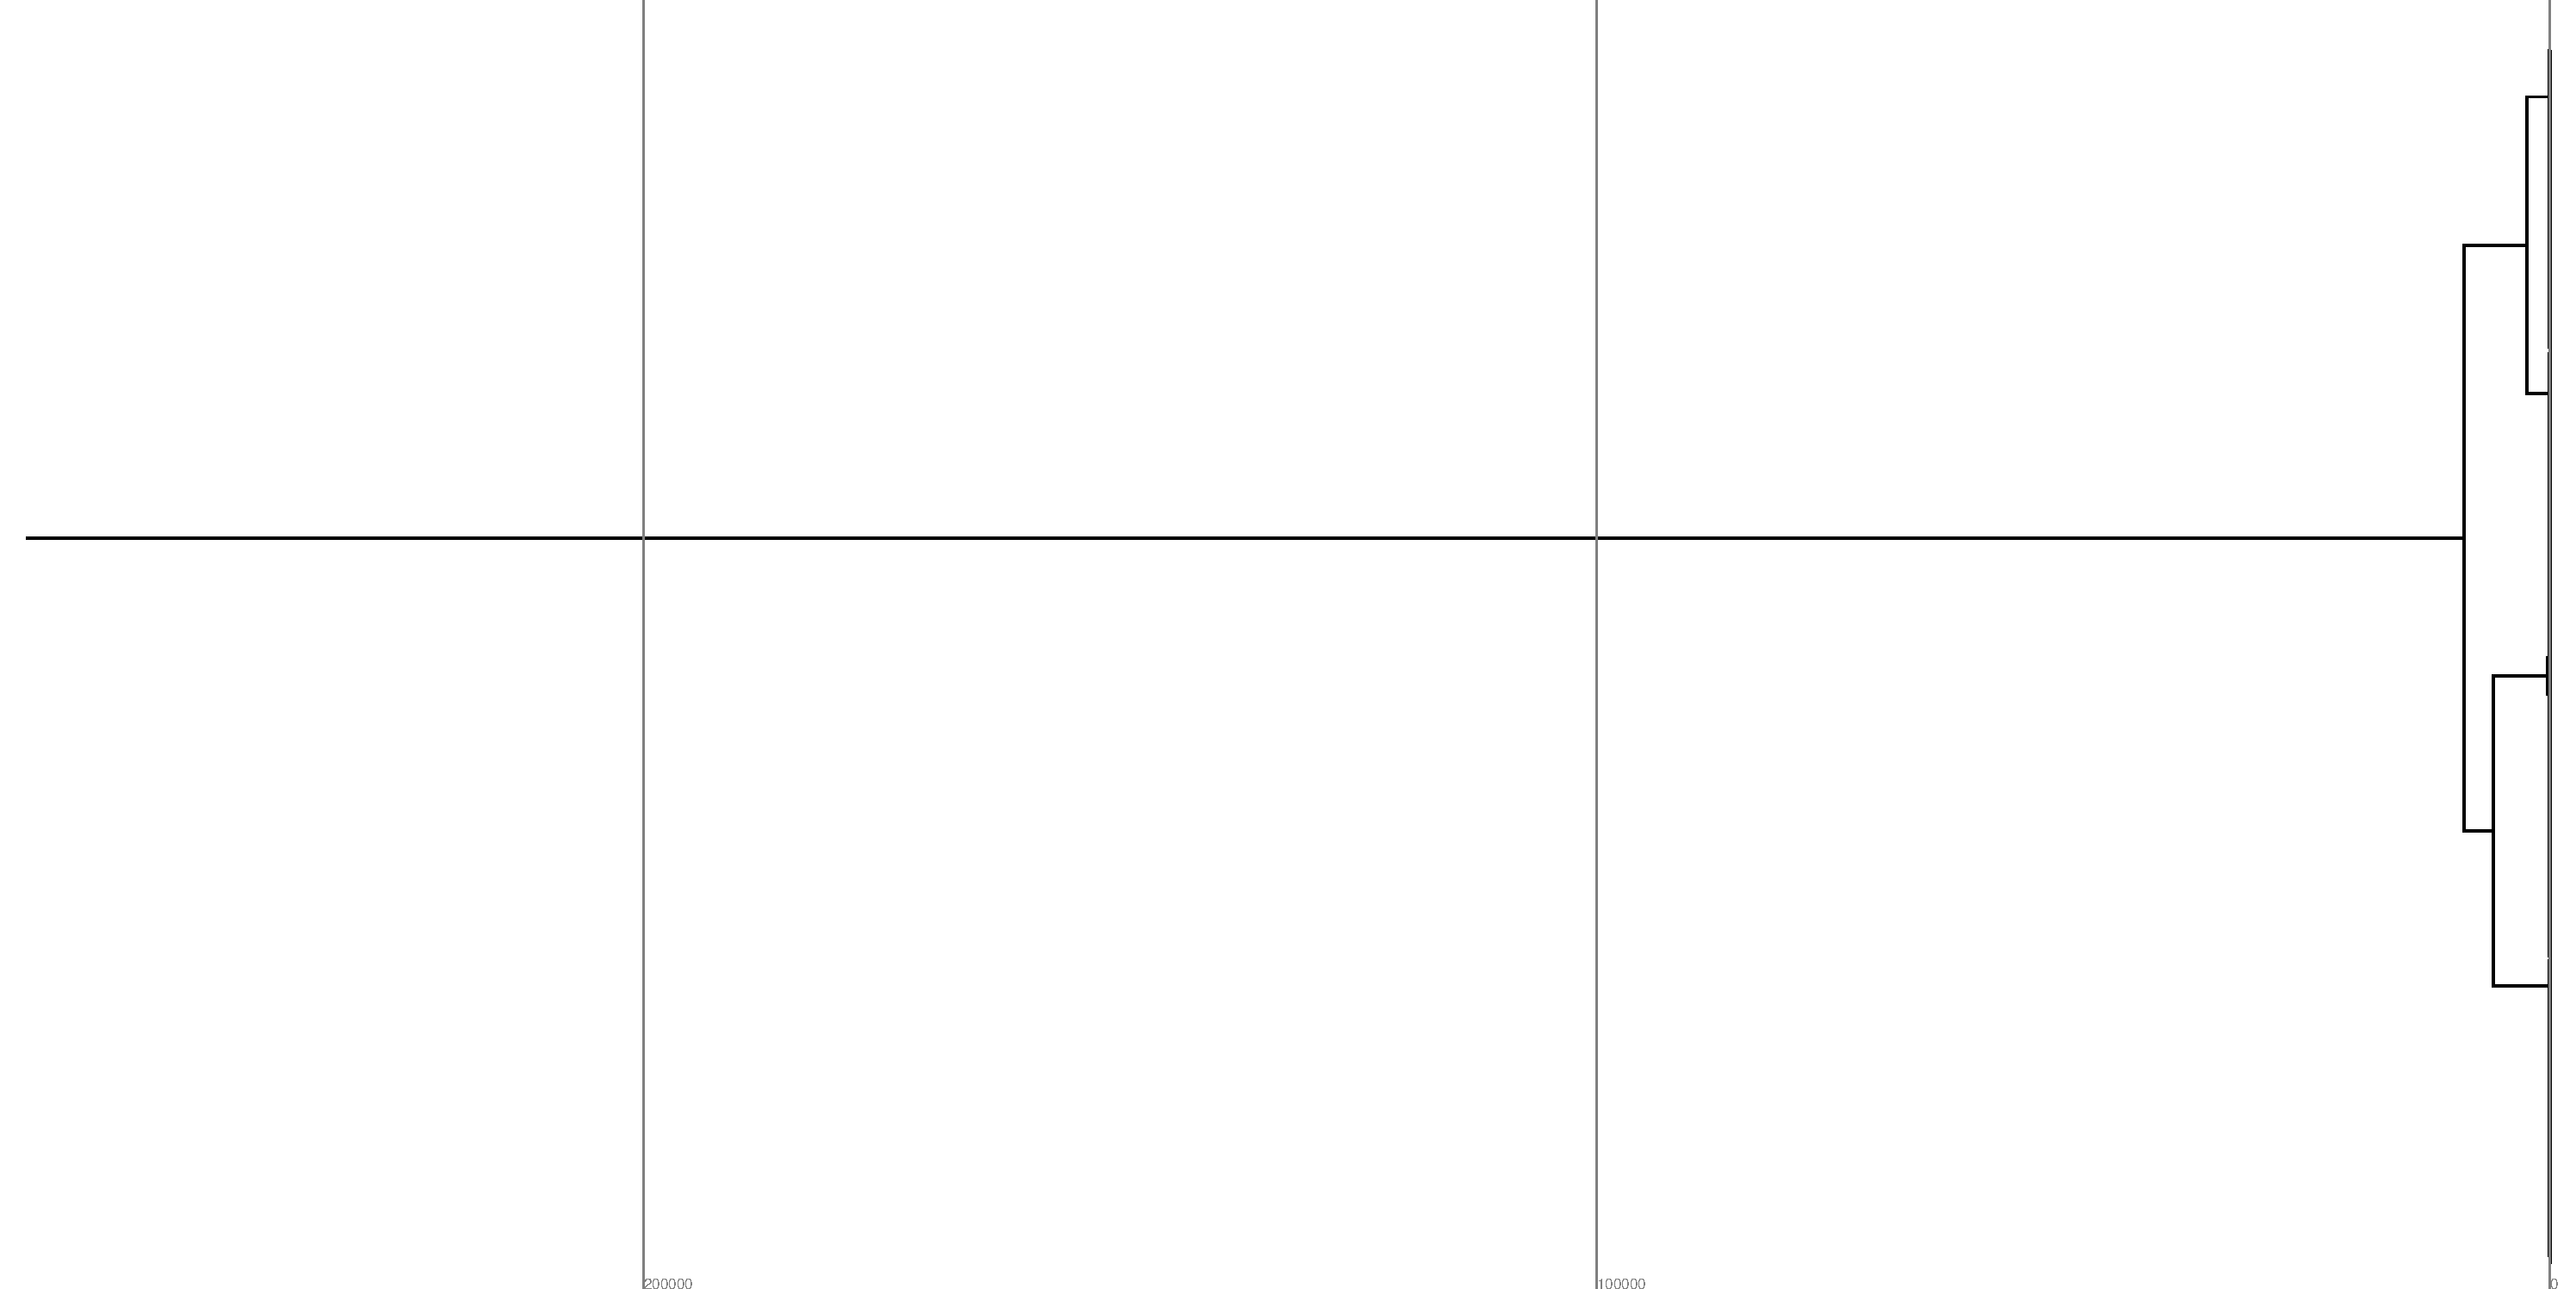
\includegraphics[height=0.12\textheight,width=\textwidth]{img/perfect-tree-phylogenies-log/epoch=7+resolution=3+treatment=4/a=collapsed-phylogeny+epoch=00007+mut_distn=np.random.standard_normal+num_generations=32768+num_islands=1+num_niches=4+p_island_migration=0.01+p_niche_invasion=3.0517578125e-08+population_size=32768+r.../eplicate=0+tournament_size=4+treatment=4+_generation=262144+_index=4+scale=nonlog+ext=.pdf}
% % \end{noindent}
% \caption{%
% 4 niche ecology strong selection}
% % \label{fig:perfect-tree-phylogenies-log:TODO}
% \end{subfigure}
% \hfill
